\documentclass[acronym,symbols,table]{fei}

%\usepackage{glossaries}
\usepackage[utf8]{inputenc}
\usepackage{subcaption} 
\renewcommand{\thesubfigure}{\Alph{subfigure}}
\usepackage{graphicx}
\usepackage{amsmath} % for the equation* environment
\usepackage{float}
\usepackage[portuguese]{algorithm2e}
\usepackage{biblatex}
\usepackage{listings}
\usepackage{chngcntr} 
\usepackage{appendix}
\usepackage{gensymb}
\counterwithout{footnote}{chapter}
\usepackage{siunitx}
\sisetup{output-exponent-marker=\ensuremath{\mathrm{e}}}
\renewcommand{\cftfigurepresnum}{Figura }
\setlength{\cftfigurenumwidth}{5.7em}
\usepackage{titling}
\usepackage{comment}

\title{Avaliação do condicionamento do ar da frota L do Metrô de São Paulo}
\author{Ana Sung Marques \\Felipe Estevão Coquito de Mello\\  Gabriel de Souza Simonetti  \\ Gabriel Mola da Silva \\ Netuno Trindade Torrente Rovaroto \\ Victor Salzo Lopes  \\ Vitoria Fedatto Stefaneli}
\cidade{São Bernardo do Campo}
\instituicao{Centro Universitário FEI}

\addbibresource{Referencias.bib}
%\bibliographystyle{plain}
\bibliography{Referencias}
\graphicspath{ {Imagens/}, {Tabelas/}}

%\makeglossaries
%%\newacronym[] {achpt} {ACT} {Aparecido ChupeTão}

\newacronym[longplural=Associações Brasileiras de Normas Técnicas]{abnt}{ABNT}{Associação Brasileira de Normas Técnicas}

\newacronym{ibge}{IBGE}{Instituto Brasileiro de Geografia e Estatística}

\newacronym{ashrae}{ASHRAE}{\textit{American Society of Heating, Refrigerating and Air-Conditioning Engineers}}

\newacronym{nbr}{NBR}{Norma Brasileira}

\newacronym{pmv}{PMV}{\textit{Predicted Mean Vote}}
	
\newacronym{ppd}{PPD}{\textit{Predicted Percentage of Dissatisfied}}
		
\newacronym{vgd}{VGD}{Ventilação Geral Diluidor}
		
\newacronym{vgl}{VGL}{Ventilação Local Exaustora}
		
\newacronym{cfd}{CFD}{\textit{Computational Fluid Dynamics}}
		
\newacronym{pcb}{PCB}{\textit{Printed Circuit Board}}
		
\newacronym{sms}{SMS}{\textit{Short Message Service}}
		
%\newglossaryentry{pi}{parent=greek,type=symbols,name={\ensuremath{\pi}},sort=p,description={número irracional que representa [razão entre a circunferência de qualquer círculo e seu diâmetro]}}
		


\begin{document}

\maketitle

\begin{folhaderosto}
	Trabalho de Conclusão de Curso apresentado ao Centro Universitário FEI, como parte dos requisitos necessários para obtenção do título de Bacharel em Engenharia Mecânica. Orientado pelo Prof. Dr. Cyro Albuquerque Neto.
\end{folhaderosto}

%\begin{agradecimentos}

%\end{agradecimentos}

\begin{resumo} %REESCREVER NO FINAL DE TUDO

Com a realização de mais de 1 bilhão de viagens o Metrô de São Paulo é uma das maiores redes de transporte público do país, com cerca de um bilhão de passageiros transportados anualmente. No entanto, ainda enfrenta um grande problema: o conforto térmico dentro dos carros. O serviço possui canais de reclamações e, segundo informações fornecidas via \textit{SMS}, no ano de 2023, o maior volume de reclamações foi em relação à ventilação e ar-condicionado. Visando melhorar o conforto térmico e a diminuição das reclamações, será realizado um estudo por meio de uma parceria do Metrô de São Paulo com o Centro Universitário FEI. Dessa forma, o objetivo principal do trabalho será analisar as condições atuais de conforto térmico para os passageiros do Metrô, buscando, assim, possíveis soluções para o sistema já existente. Para atingir o objetivo proposto, torna-se necessária a utilização de sensores para medir determinadas propriedades do ar, correlacionando-as com reclamações dos passageiros e a norma técnica vigente. Nesse contexto, o trabalho tem como principal meta o desenvolvimento de placas de sensoriamento que permita analisar as propriedades do ar, tais como: temperatura, umidade, concentração de $CO_2$ e produção de contaminantes. Posteriormente, os sensores deverão ser posicionados dentro dos carros do Metrô, permitindo a coleta dos dados e comparando-os com as normas utilizadas atualmente, no caso, a NBR-16.401-2 e a \textit{ASHRAE}. Em uma etapa mais avançada, o sistema será estudado mediante simulações de elementos finitos no \textit{Software Ansys}, visando observar se o posicionamento dos dutos de insuflamento e exaustão são realmente eficientes. 

\palavraschave{Metrô. Condicionamento de ar. Transporte público.}

\end{resumo}

\begin{abstract} %REESCREVER  NO FINAL DE TUDO

With an annual ridership of approximately one billion passengers, the Metrô de São Paulo is recognized as the largest public transportation system in Brazil. However, it continues to face a persistent challenge regarding the thermal comfort within its train cars. The service has established a specific channel for customer complaints. Analysis of \textit{SMS} complaints received in 2023 indicates that 20\% pertain to issues with air conditioning and ventilation. To improve thermal comfort and reduce the volume of complaints, a collaborative research initiative will be undertaken by Metrô de São Paulo in partnership with Centro Universitário FEI. This project will involve the deployment of sensors to assess various air quality parameters, linking these measurements to passenger feedback and current technical standards. The primary goal of this initiative is to create sensor boards that enable the monitoring of air characteristics, including temperature, humidity, $CO_2$ levels, and the presence of contaminants. Subsequently, these sensors will be installed in subway cars to gather data that can be evaluated against established standards, specifically NBR-16.401-2 and \textit{ASHRAE}. In a later phase, the system will undergo analysis through finite element simulations using \textit{Software Ansys}, to determine the effectiveness of the placement of supply and exhaust ducts.

    \keywords{Metro. Air conditioning. Public transport.} 

\end{abstract}

\listoffigures
\listoftables
%\printglossaries
%\printglossary[type=\acronymtype]
\tableofcontents

\chapter{Introdução}

A Companhia do Metropolitano de São Paulo – Metrô teve sua primeira atividade no dia 14 de setembro de 1974, e é considerada um incrível marco na engenharia e planejamento urbano \cite{inicio}. Ela surgiu como uma solução vital para o transporte das inúmeras pessoas na região metropolitana de São Paulo, que posteriormente com o rápido crescimento populacional, este meio de transporte se tornou cada vez mais essencial na vida dos paulistas. 

No entanto, por mais que o metrô seja uma excelente proposta para mitigar os problemas de tráfego e transporte enfrentados na metrópole, ele enfrenta diversos desafios, incluindo a lotação em horários de pico, com milhões de pessoas fazendo uso deste meio de transporte todos os dias, além da necessidade de melhoria na manutenção e infraestrutura.

Considerando a enorme quantidade de pessoas utilizando este meio de transporte, um dos maiores adversidades para os responsáveis é fornecer ambientes internos agradáveis e seguros. Isso destaca ainda mais a necessidade de estudar a respeito do conforto térmico e a qualidade do ar dentro dos vagões, para avaliar a situação atual e desenvolver e proporcionar uma solução para esta problemática.

\section{Motivação}

A cidade de São Paulo é a maior cidade do Brasil, com mais de 11 milhões de habitantes \cite{IBGE},  e com seu crescimento acelerado se faz necessário abordar discussões a respeito de soluções para a mobilidade urbana na cidade. Portanto, cria-se a necessidade de incentivar a utilização de transportes coletivos. Desse modo, proporcionar uma experiência agradável nos transportes públicos auxilia no desenvolvimento positivo da mobilidade urbana de São Paulo,trazendo mais pessoas para os transportes coletivos.

Segundo o \textcite{cnt} os transportes públicos foram responsáveis por 15,3 milhões de viagens diárias no ano de 2017 na grande São Paulo, o que equivale a um total de 37\% do total dos deslocamentos da cidade, Figura \ref{fig:cnt}. Os serviços de trilhos tendo aproximadamente 4 milhões de viagens diárias o que corresponde a 25\% entre os transportes públicos. Considerando esse número expressivo o suficiente os serviços oferecidos pelo Metrô de São Paulo são fundamentais para a vida das pessoas atualmente, logo é essencial olhar as problemáticas que o mesmo possui.

\begin{figure}[!htb] 
 \centering
    \caption{Distribuição das viagens na grande São Paulo}
    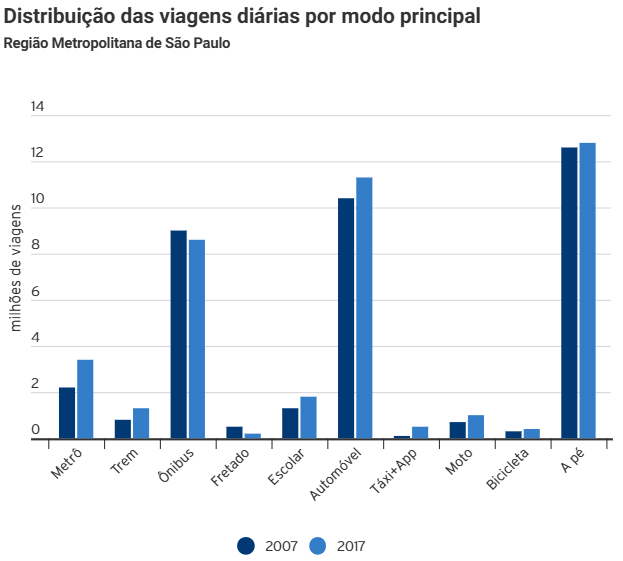
\includegraphics[width=0.8\linewidth]{Imagens/Distruibuicao.png}
    \smallcaption{Fonte: \textcite{cnt}}
    \label{fig:cnt}
\end{figure}

\newpage 

No portal oficial \textcite{MetroSP} uma das maiores problemáticas atribuídas ao Metrô de São Paulo reside na qualidade do ar e na temperatura interna nos vagões, no ano de 2023 do total de 42380 reclamações, 21\% foram referentes a ar-condicionado dentre estas a principal queixa referente ao calor, com mais de 8 mil reclamações, é possível observar essas informações nas Figuras \ref{fig:grafico_total} e \ref{fig:grafico_ar}. Logo com essa questão ressaltada, a urgência de um estudo que proponha a solução para os problemas de ventilação dentro dos vagões da frota do metrô é palpável.

\begin{figure}[!htb]
	\centering
	\begin{minipage}{0.5\textwidth}
		\caption{Reclamações totais do Metrô de São Paulo no ano de 2023}
		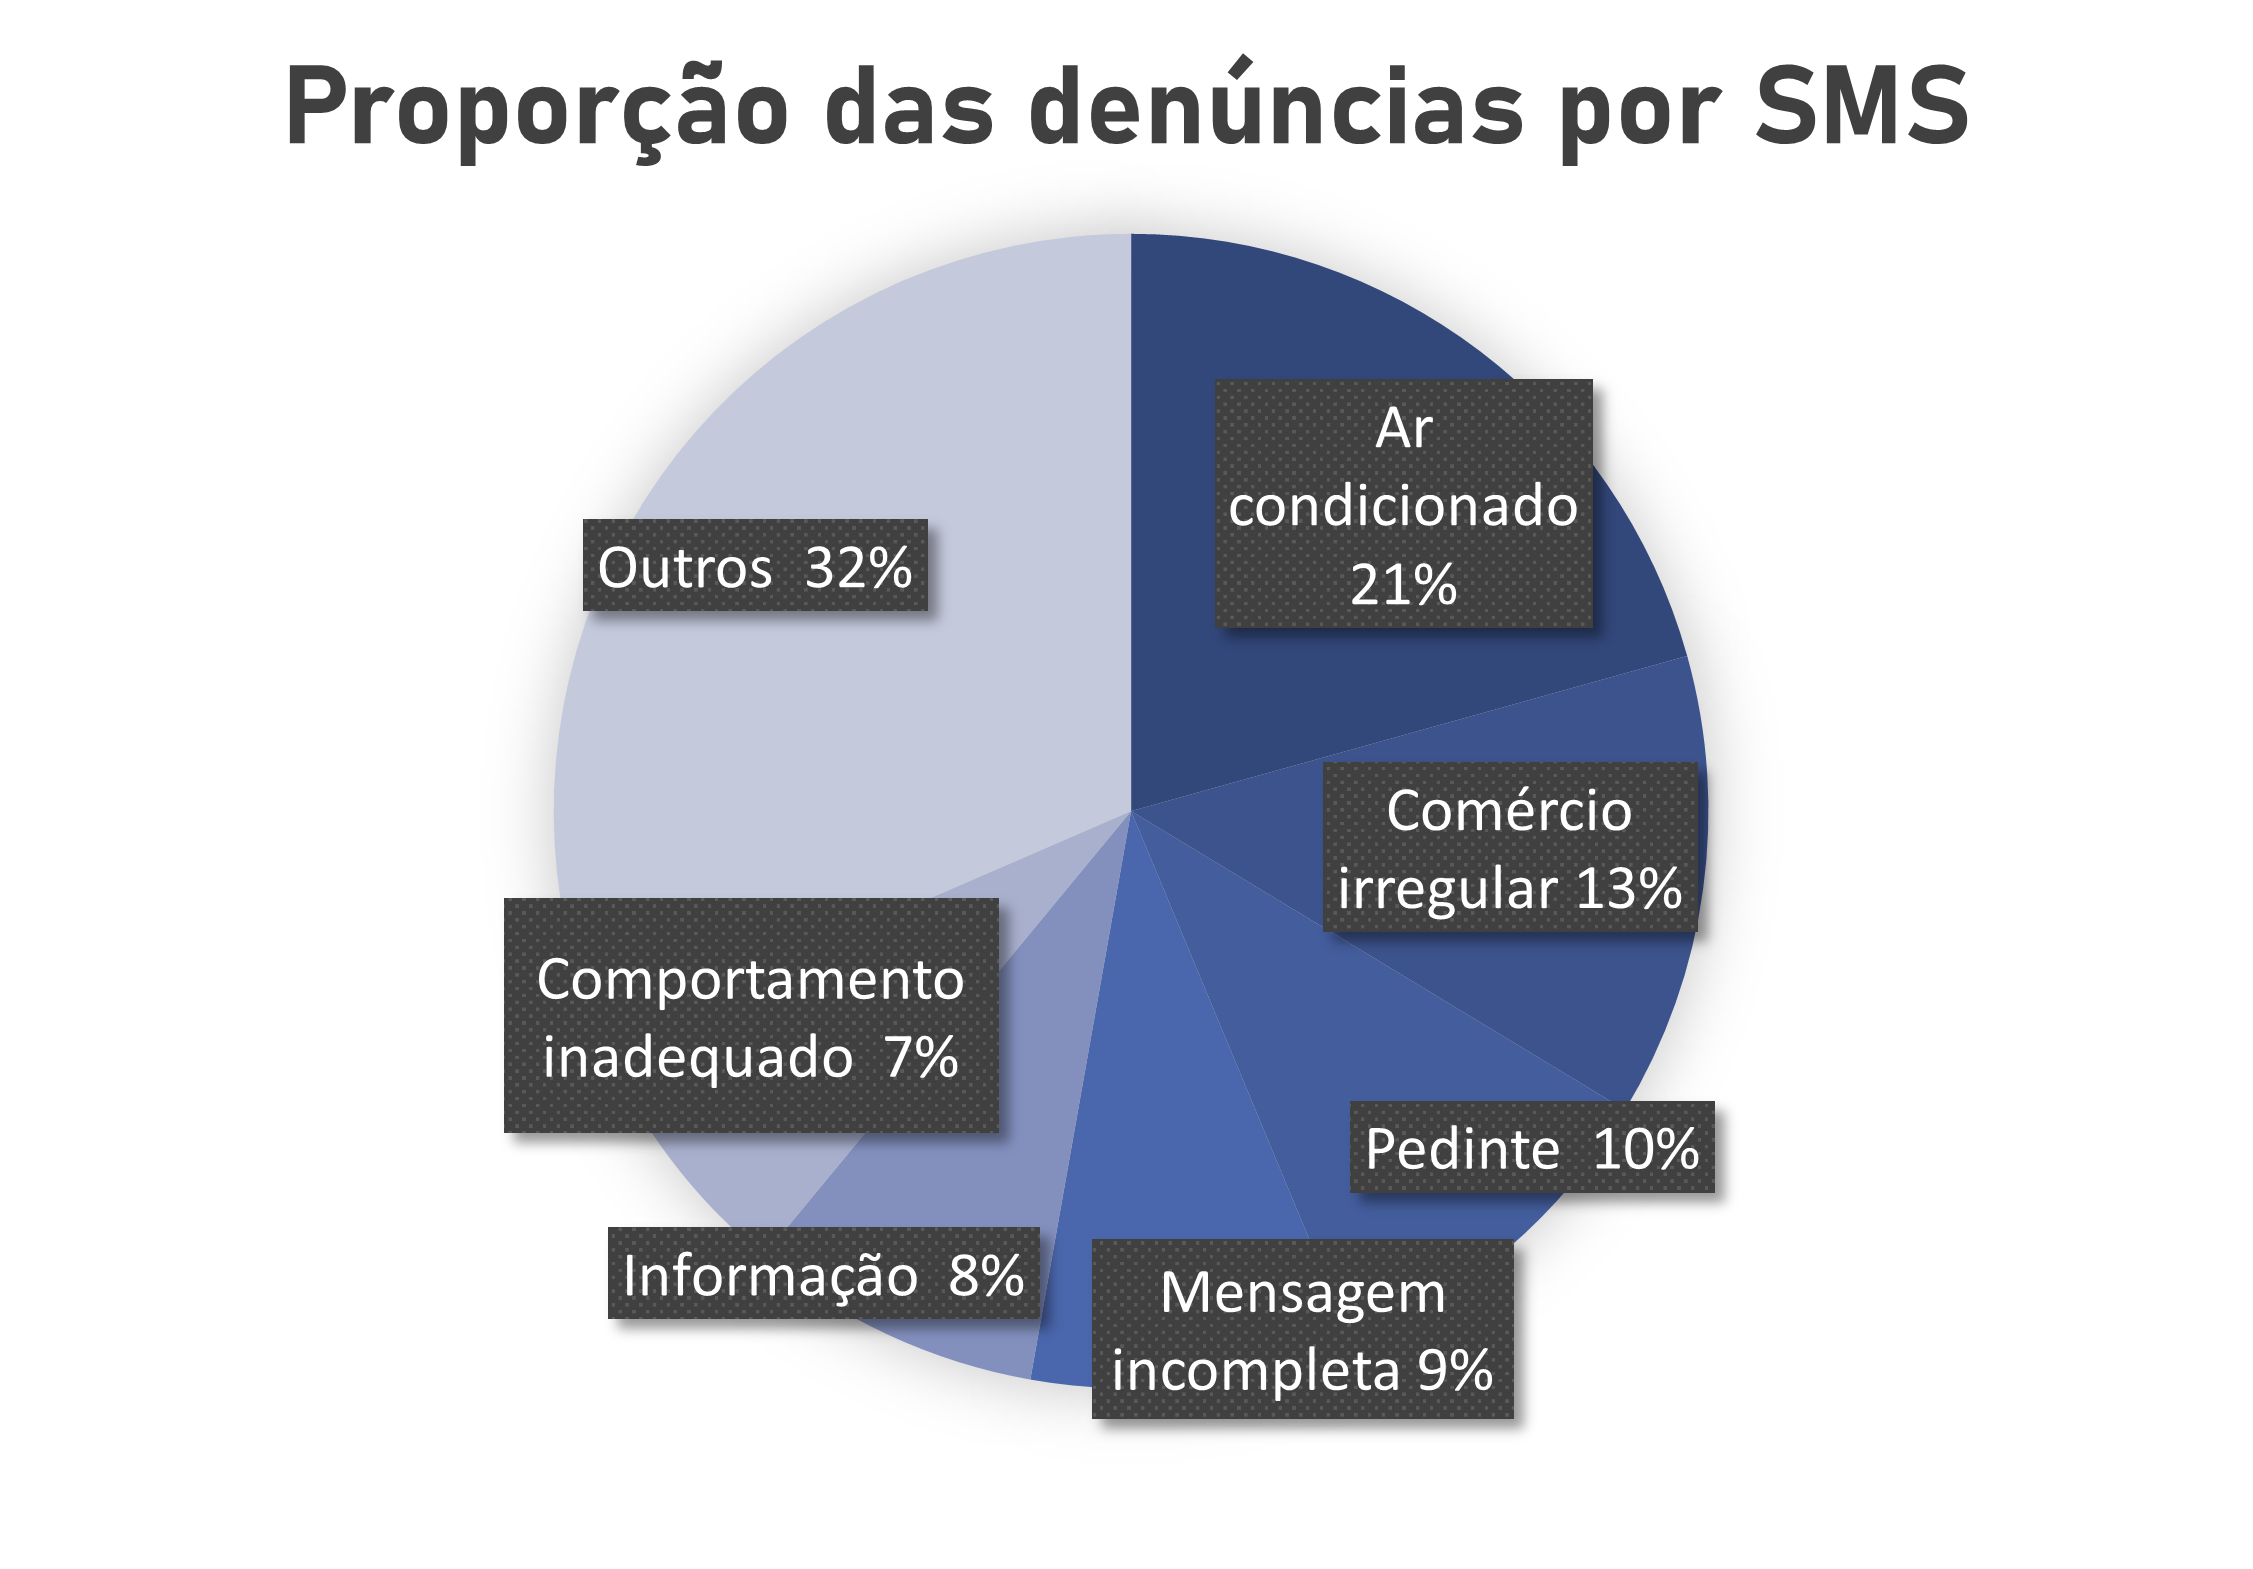
\includegraphics[width=\linewidth, height=6cm]{Imagens/Grafico_reclamacoes_totais.png}
		\smallcaption{Fonte: \textcite{metrosp2024}}
		\label{fig:grafico_total}
	\end{minipage}\hfill
	\begin{minipage}{0.45\textwidth}
		\caption{Reclamações de ar-condicionado do Metrô de São Paulo no ano de 2023}
		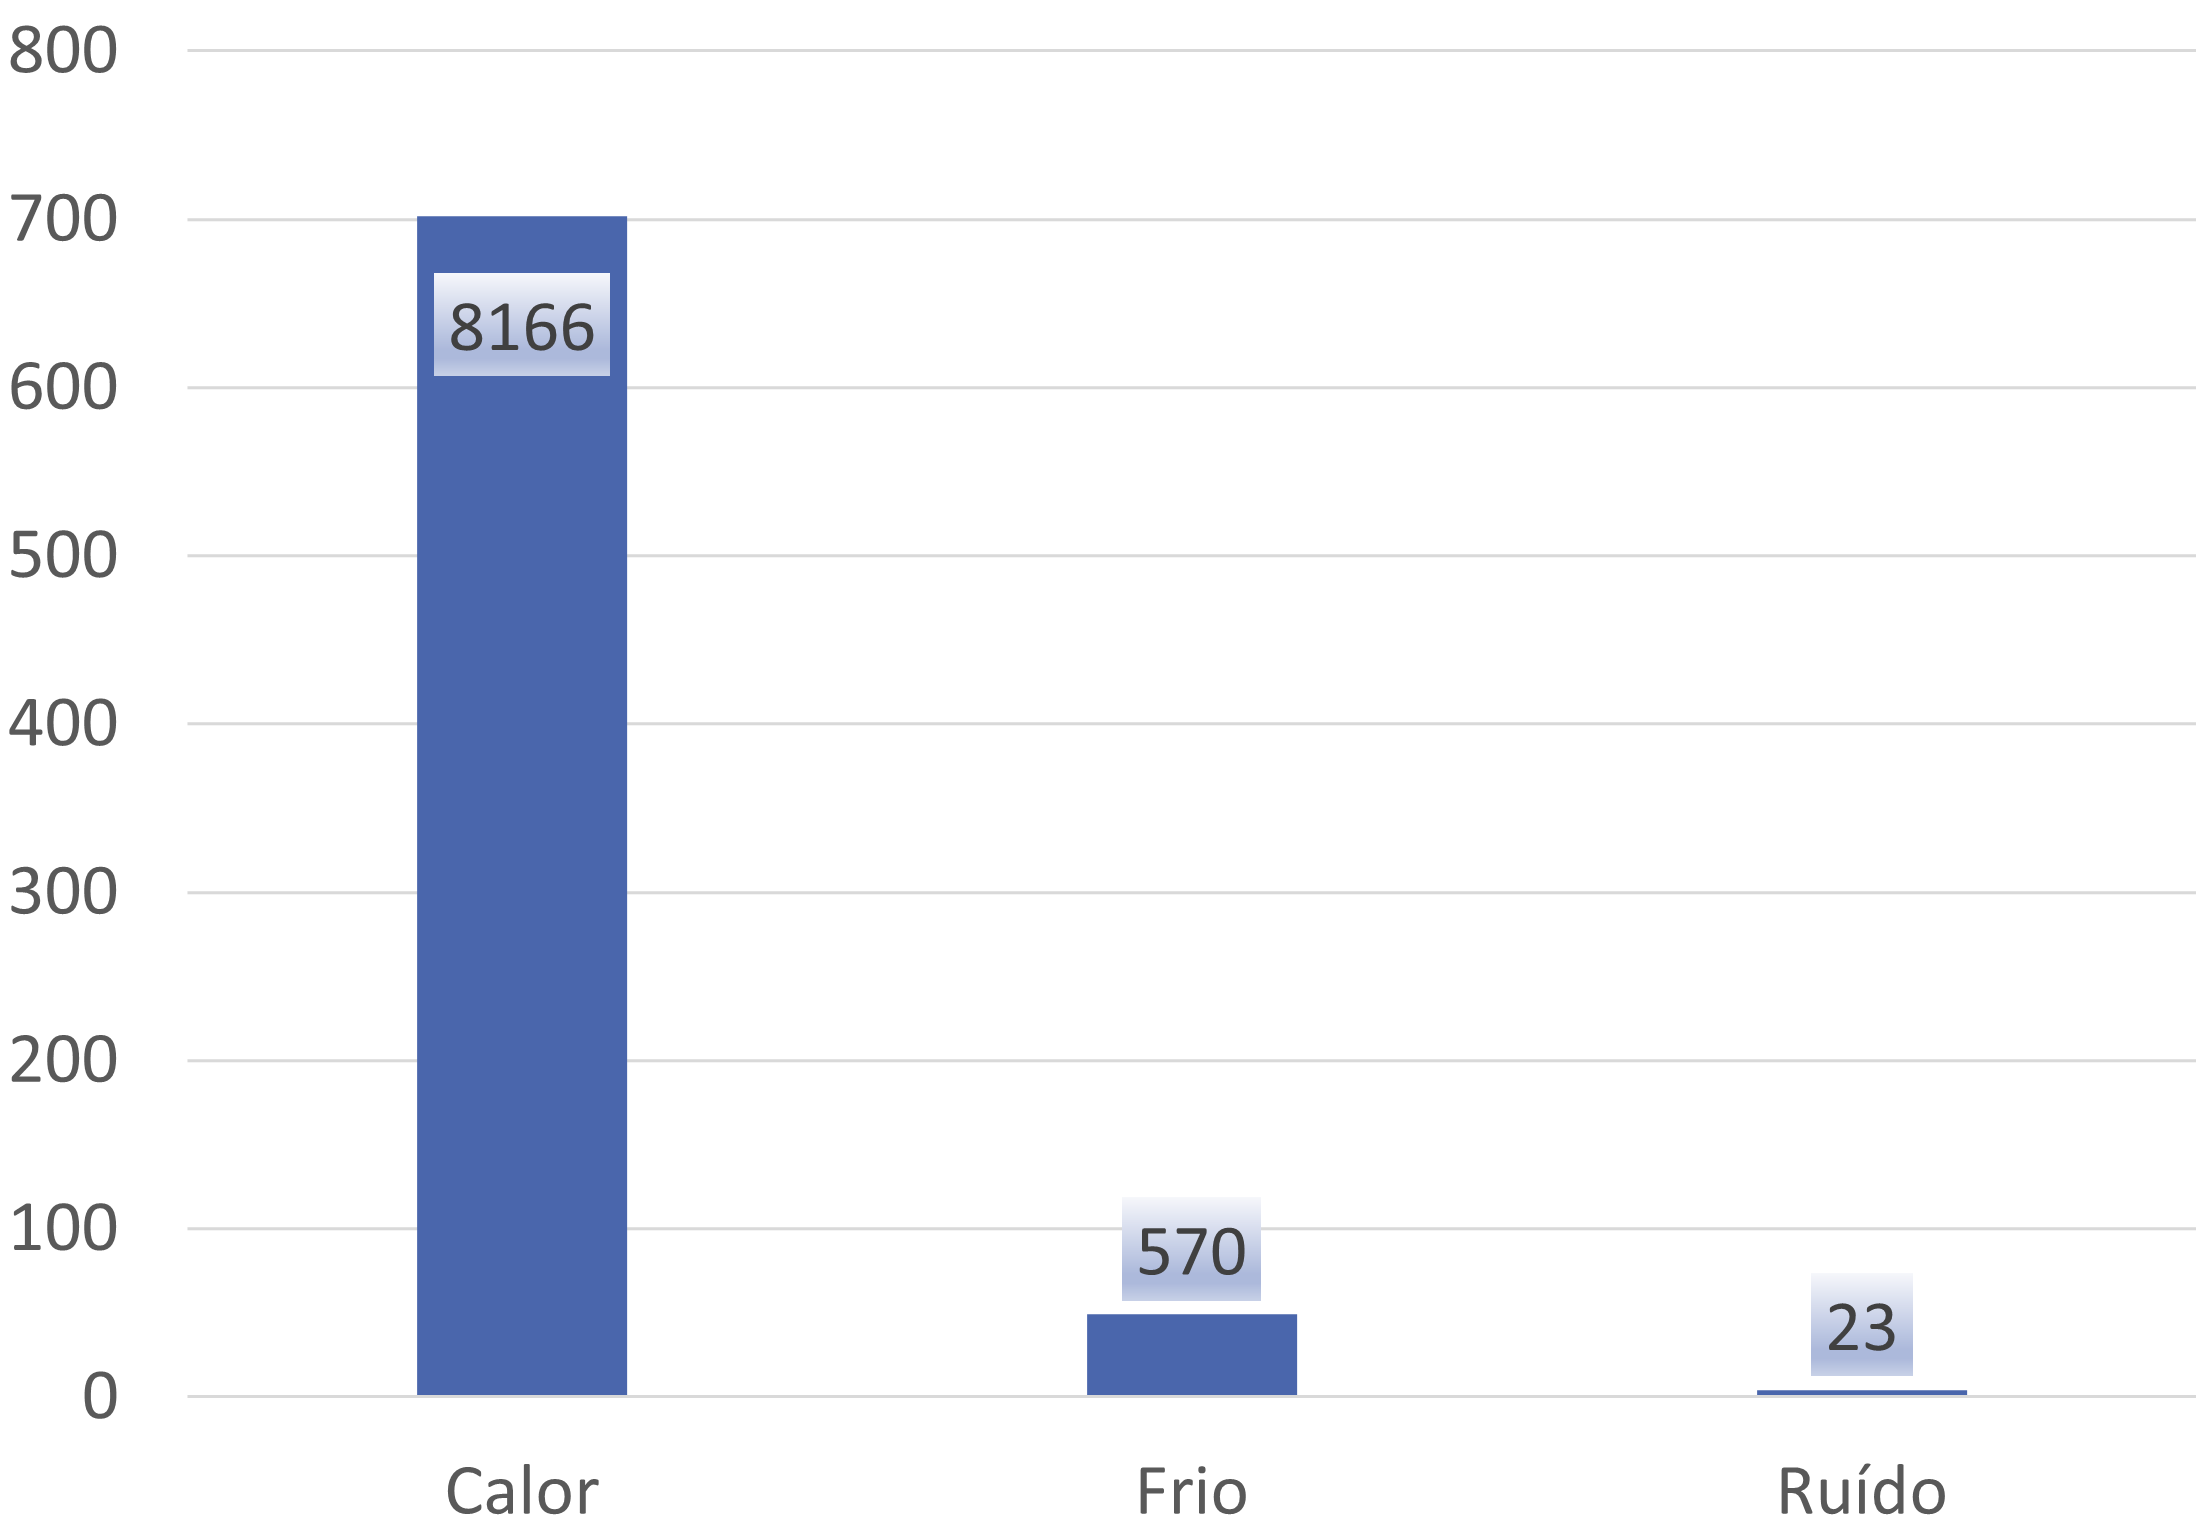
\includegraphics[width=\linewidth, height=6cm]{Imagens/Grafico_reclamacoes_ar.png}
		\smallcaption{Fonte: \textcite{metrosp2024}}
		\label{fig:grafico_ar}
	\end{minipage}
\end{figure}

\newpage 

\section{Objetivo geral}

O objetivo deste trabalho é realizar, através de dados de sensoriamentos do interior e exterior aos vagões do Metrô da Frota L, uma análise do condicionamento de ar e do conforto térmico dos passageiros, entendendo assim quais são os parâmetros que influenciam em suas experiências. Pretende-se correlacionar os dados obtidos com as reclamações recebidas por meio do canal de denúncias do Metrô via \textit{SMS}, visando compreender a percepção dos passageiros de forma qualitativa. Além disso, será realizada a avaliação das condições térmicas dos vagões e sua conformidade com as normas, se apoiando nos cálculos teóricos realizados para que se possam sugerir melhorias e oportunidades para estudos futuros. 

\section{Objetivos específicos}

\begin{itemize}
    \item[1 -]Reunião com a equipe do Metrô de São Paulo para, alinhamento de ideias e posteriormente a  aquisição dos dados relevantes para o trabalho, tais como: reclamações via \textit{SMS}, estatísticas a respeito do Metrô de São Paulo, desenhos do equipamento de Aquecimento, Ventilação e Ar-condicionado (AVAC), peso dos vagões ao longo do tempo,temperaturas ao longo do tempo;
    \item[2 -]Início do tratamento e análise de dados oferecidos pelo Metrô de São Paulo, cálculos teórico de acordo com as normas;
    \item[3 -]Desenvolvimento de placas de sensoriamento com base em \textit{Arduino}, posicionadas em locais estratégicos do vagão, visando medir propriedades adicionais a serem observadas, tais como: temperatura, umidade, concentração de gás carbônico e pressão barométrica;
    \item[4 -]Visita técnica no Metrô de São Paulo, buscando estudar o melhor posicionamento dos sensores mencionados, evitando, desta forma, desvios na aquisição dos dados;
    \item[5 -]Coleta, interpretação e análise detalhada dos dados da instrumentação;
    \item[6 -]Estudo adicional realizado através do \textit{Software Ansys}, visando melhor visualização dos dados e do comportamento do sistema;
    \item[7 -]Comparação de todos os dados coletados, calculados e tratados para uma análise completa do condicionamento de ar e do conforto térmico dos passageiros e observar se há conformidade com as normas;
    \item[8 -]Possíveis sugestões de melhoria para o sistema.
\end{itemize}

\section{Estrutura da Monografia} %REESCREVER  NO FINAL DE TUDO

No Capítulo 2 é feito o estudo do referencial teórico das normas para conforto térmico e toda a teoria que ela carrega consigo, além dos conceitos de analises computacionais. No Capítulo 3 é apresentada a metodologia do trabalho, onde estão descritas as coletas de dados os sensores utilizados, os testes e simulações e os cálculos a serem realizados. No Capítulo 4 são demonstrados os resultados de cada uma das áreas do projeto. No Capítulo 5 são elaboradas as conclusões cruzando os resultados de cada área do trabalho e buscando encontrar correlações. O Capítulo 6 finaliza o trabalho com as possibilidades de trabalhos futuros a partir do que foi desenvolvido.

\chapter{Referências Bibliográficas}

Para se conseguir um ambiente termicamente agradável é necessário avaliar alguns parâmetros e condições do ar. Para isso, leva-se em consideração a ventilação, as trocas de calor com o ambiente, as produções de energia térmica, os contaminantes e taxas metabólicas. Portanto, aplica-se balanços de energia para se calcular o conforto térmico no espaço.

\section{Leis Fundamentais da Termodinâmica} 

As leis fundamentais da termodinâmica buscam descrever as características e transformações da energia. Neste contexto, a Primeira Lei da Termodinâmica refere-se à conservação da energia, isto é, em uma interação, a energia pode alterar sua forma, porém, a quantidade total permanece a mesma e, portanto, a energia não pode ser criada ou destruída \cite{cengel1998heat}. Dessa maneira, a variação de energia é descrita como uma subtração entre a quantidade de entrada e saída no sistema, visto na Equação \ref{eq: energia}.

\begin{equation} \label{eq: energia}
    \begin{aligned}
    \Delta E = E_{\text{entrada}} - E_{\text{saída}}
    \end{aligned}
\end{equation}


Por sua vez, a Segunda Lei da Termodinâmica determina que o fluxo de calor direciona-se do corpo de temperatura mais alta para o de menor temperatura \cite{cengel1998heat}, além de incorporar o conceito de rendimento, no qual máquinas são incapazes de converter todo o calor em trabalho útil.

\section{Mecanismos de Transferência de Calor} 

A transferência de calor refere-se ao modo como o calor é transmitido entre os meios e pode ocorrer de três formas distintas, sendo elas: condução, convecção e radiação.

Em gases e líquidos, a condução ocorre através da colisão entre moléculas durante seu movimento aleatório, ao passo que, em sólidos, a mesma se dá pela vibração das moléculas, transportando energia pelos elétrons livres \cite{cengel1998heat}. A taxa de transferência de calor por condução ($\dot{Q}_{cond}$) pode ser determinada através da Lei de Fourier conforme a Equação \ref{eq:Condução}.

\begin{equation} \label{eq:Condução}
\begin{aligned}
    \dot{Q}_{\text{cond}} = k_{t} \cdot A_{\text{cond}} \cdot \frac{\Delta T}{\Delta x}
\end{aligned}
\end{equation}

Dessa maneira, o gradiente de temperatura e a espessura da camada a ser atravessada se relaciona à condutividade térmica do material ($k_{t}$) e área normal à direção da transferência de calor ($A_{cond}$). Entretanto, pode-se considerar uma resistência à condução do material representada na Equação \ref{eq:Rcondução}.

\begin{equation} \label{eq:Rcondução}
\begin{aligned}
    {R}_{k}=\frac{\Delta x}{k_{t} \cdot A}
\end{aligned}
\end{equation}

Assim, a Equação \ref{eq:Condução} pode ser reescrita como, a Equação \ref{eq:Condução_Req}:

\begin{equation} \label{eq:Condução_Req}
\begin{aligned}
    \dot{Q}_{\text{cond}} = \frac{\Delta T}{{R}_{k}}
\end{aligned}
\end{equation}

A Tabela \ref{tab:Condutividade_Termica} indica a condutividade térmica de alguns materiais comumente utilizados no cotidiano.

\begin{table}[!htb] 
 \centering
    \caption{Condutividade térmica de materiais à temperatura ambiente}
    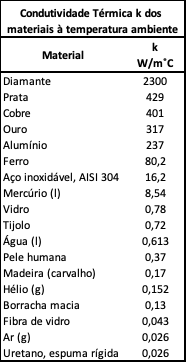
\includegraphics[width=0.4\linewidth]{Tabelas/Condutividade_Termica.png}
    \smallcaption{Fonte: Autor. Adaptado de \textcite{ccengel2008heat}}
    \label{tab:Condutividade_Termica}
\end{table}

Já a convecção trata-se da transferência de energia entre uma superfície sólida e o líquido ou gás adjacente à superfície. Assim, pode-se classificar a convecção como natural, quando ocorre devido à diferença de densidades ocasionada pela disparidade de temperaturas, ou como forçada que, por sua vez, envolve meios externos para provocar o escoamento do fluido ao longo da superfície \cite{kreith1999mechanical}. A taxa de transferência de calor por convecção ($\dot{Q}_{conv}$) pode ser determinada através da Lei de Resfriamento de Newton conforme Equação \ref{eq:Convecção}.

\begin{equation} \label{eq:Convecção}
\begin{aligned}
    \dot{Q}_{conv}=h \cdot A_{s} \cdot (T_{s}-T_{f})
\end{aligned}
\end{equation}

Deste modo, tem-se o coeficiente de transferência de calor por convecção ($h$) multiplicado pela área da superfície na qual ocorre a troca de calor ($A_{conv}$) e pela diferença entre as temperaturas da superfície ($T_{s}$) e do fluido ao longe ($T_{f}$), o qual se encontra distante o suficiente para não realizar trocas de calor por condução. Pelo mesmo raciocínio utilizado anteriormente, pode-se determinar uma resistência à convecção conforme Equação \ref{eq:Rconvecção}.

\begin{equation} \label{eq:Rconvecção}
\begin{aligned}
    {R}_{c}=\frac{1}{h \cdot A}
\end{aligned}
\end{equation}

E, portanto, a Equação \ref{eq:Convecção} pode ser reescrita como a Equação \ref{eq:Convecção_Req}:

\begin{equation} \label{eq:Convecção_Req}
\begin{aligned}
    {Q}_{conv}=\frac{T_{s}-T_{f}}{{R}_{c}}
\end{aligned}
\end{equation}

Vale ressaltar que o cálculo do coeficiente de convecção depende de alguns fatores como tipo de escoamento, geometria do corpo e área de escoamento e propriedades físicas do fluido \cite{ozicsik1993heat}. Considerando-se convecção forçada em placas planas, na qual tem-se um fluxo de ar paralelo a uma superfície, deve-se primeiro estabelecer o número de Nusselt que, por sua vez, está atrelado ao número de Reynolds e Prandtl. O número de Reynolds em um determinado ponto $x$ ao longo do escoamento na placa é descrito conforme Equação \ref{eq:Reynolds}, na qual $\rho$ representa a densidade do fluido, $V$ a velocidade, e $\mu$ a viscosidade dinâmica.

\begin{equation} \label{eq:Reynolds}
\begin{aligned}
    {Re}_{x}=\frac{\rho \cdot V \cdot x}{\mu}
\end{aligned}
\end{equation}

Já o número de Prandtl refere-se a uma grandeza adimensional, relacionando a espessura relativa da velocidade e das camadas limite térmicas \cite{cengel1998heat}. A Tabela \ref{tab: Propriedades_Ar} demonstra valores usuais de propriedades do ar utilizados nos cálculos de Reynolds, além do número de Prandtl de acordo com a temperatura do ar.

\begin{table}[!htb] 
 \centering
    \caption{propriedades do ar a 1 atm}
    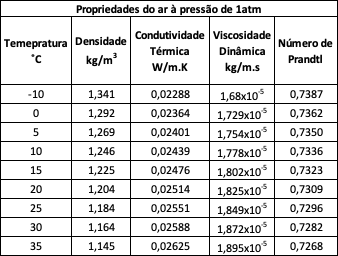
\includegraphics[width=0.7\linewidth]{Tabelas/Propriedades_ar_1atm.png}
    \smallcaption{Fonte: Autor. Adaptado de \textcite{ccengel2008heat}}
    \label{tab: Propriedades_Ar}
\end{table}

Considerando-se escoamento laminar, no qual Reynolds é menor que $5 \cdot 10^5$, pode-se determinar o número médio de Nusselt ao longo de toda a placa de comprimento $L$ conforme a Equação \ref{eq:Nusselt_Laminar}.

\begin{equation} \label{eq:Nusselt_Laminar}
\begin{aligned}
    Nu=0,664 \cdot Re_{L}^{0,5} \cdot Pr^{1/3}
\end{aligned}
\end{equation}

Para o escoamento turbulento, representado por Reynolds entre $5 \cdot 10^5$ e $10^7$ e Prandtl entre $0,6$ e $60$, o cálculo é representado pela Equação \ref{eq:Nusselt_Turbulento}.

\begin{equation} \label{eq:Nusselt_Turbulento}
\begin{aligned}
    Nu=0,037 \cdot Re_{L}^{0,8} \cdot Pr^{1/3}
\end{aligned}
\end{equation}

Dessa maneira, o coeficiente de convecção médio ao longo da placa pode ser descrito conforme Equação \ref{eq:coef. convecção}, na qual $k_{f}$ representa a condutividade térmica do fluido na média de temperatura entre a superfície e do fluido ao longe.

\begin{equation} \label{eq:coef. convecção}
\begin{aligned}
    h=\frac{k_{f} \cdot Nu}{L}
\end{aligned}
\end{equation}

Por fim, a radiação está atrelada à emissão de energia através de ondas eletromagnéticas. Vale ressaltar que todos os corpos com temperatura acima do zero Kelvin emitem radiação térmica \cite{kreith1999mechanical}. Neste contexto, sucedem os conceitos de emissividade ($\epsilon$) e absortividade ($\alpha$), os quais referem-se a medidas, determinadas entre zero e um, da capacidade de um corpo de emitir e absorver radiação, respectivamente. Assim, um corpo negro apresenta valor equivalente a um tanto para emissividade quanto absortividade e, portanto, representa uma situação ideal, emitindo radiação na taxa máxima, assim como absorvendo toda a radiação que incide sobre ele. 

Para situações em que a vizinhança possui dimensões muito maiores que a superfície e os meios são separados por um gás que não interfere na radiação, a taxa de transferência de calor por radiação ($\dot{Q}_{rad}$) pode ser definida pela Equação \ref{eq:Radiação}.

\begin{equation} \label{eq:Radiação}
\begin{aligned}
    \dot{Q}_{rad}=\epsilon \cdot \sigma \cdot A_{s} \cdot (T_{s}^4-T_{viz}^4)
\end{aligned}
\end{equation}

Nota-se que a determinação da radiação envolve a constante de Stefan-Boltzmann ($\sigma$), assim como as características da superfície e a temperatura da vizinhança ao seu redor ($T_{viz}$). Por sua vez, a resistência à radiação é determinada conforme Equação \ref{eq:Rradiação_R}.

\begin{equation} \label{eq:Rradiação_R}
\begin{aligned}
    {R}_{r}=\frac{1}{h_{rad} \cdot A}
\end{aligned}
\end{equation}

Na qual o coeficiente de radiação ($h_{rad}$) refere-se a uma simplificação, na Equação \ref{eq:h_rad}:

\begin{equation} \label{eq:h_rad}
\begin{aligned}
    {h}_{rad}=\epsilon \cdot \sigma \cdot (T_{s}^2+T_{viz}^2) \cdot (T_{s}+T_{viz})
\end{aligned}
\end{equation}

Logo, a Equação \ref{eq:Radiação_Req} pode ser reescrita:

\begin{equation} \label{eq:Radiação_Req}
\begin{aligned}
    \dot{Q}_{rad}=\frac {T_{s}-T_{viz}}{{R}_{r}}
\end{aligned}
\end{equation}

Considerando-se que a transferência total de calor representa a soma das contribuições de cada mecanismo, para simplicidade e conveniência, é comumente adotado um coeficiente de transferência de calor combinado ($h_{comb}$), o qual permite o cálculo da transferência de calor envolvendo a convecção e a radiação térmica simultaneamente \cite{yunus2003heat}, conforme Equação \ref{eq:Combinado}.

\begin{equation} \label{eq:Combinado}
\begin{aligned}
    \dot{Q}_{conv+rad}=h_{comb} \cdot A_{s} \cdot (T_{s}-T_{f})
\end{aligned}
\end{equation}

Um termo importante no conceito de transferência de calor refere-se ao coeficiente global de transferência de calor ($\overline{U}$), derivado de uma modificação da Lei de Resfriamento de Newton \cite{kreith1999mechanical}, conforme Equação \ref{eq:Q_Global}.

\begin{equation} \label{eq:Q_Global}
\begin{aligned}
    \dot{Q}=\overline{U} \cdot A \cdot \Delta T
\end{aligned}
\end{equation}

A Equação \ref{eq:coef. U} especifica o cálculo usualmente utilizado para obter o coeficiente global de transferência de calor, envolvendo a combinação das resistências térmicas do sistema, as quais resultam em uma resistência térmica equivalente ($R_{eq}$).

\begin{equation} \label{eq:coef. U}
\begin{aligned}
    \overline{U} \cdot A=\frac{1}{R_{eq}}
\end{aligned}
\end{equation}

E, portanto, a Equação \ref{eq:Q_Global} pode ser reescrita na Equação \ref{eq:Q_Req}:

\begin{equation} \label{eq:Q_Req}
\begin{aligned}
    \dot{Q}=\frac{\Delta T}{R_{eq}}
\end{aligned}
\end{equation}

Deste modo,  assemelhando-se à elétrica, resistências térmicas em série referem-se a um único sentido sequencial de fluxo de calor ao passo que as associações em paralelo, como o próprio nome diz, se caracterizam por um fluxo de calor que se divide, sendo transferido em linhas paralelas. Assim, as equações de resistências equivalentes em série e paralelo são determinadas nas Equações \ref{eq:Req_serie} e \ref{eq:Req_paralelo}, respectivamente, sendo $n$ o número de resistências presentes no sistema.

\begin{equation} \label{eq:Req_serie}
\begin{aligned}
    {R}_{eq(serie)}=\sum^{n}_{i=1}{R_{i}}
\end{aligned}
\end{equation}

\begin{equation} \label{eq:Req_paralelo}
\begin{aligned}
    {R}_{eq(paralelo)}=\sum^{n}_{i=1}{\frac{1}{R_{i}}}
\end{aligned}
\end{equation}

Neste contexto, vale notar que nem sempre a determinação da resistência é um processo simples, especialmente para a convecção, uma vez que a velocidade do fluido e temperatura da superfície podem difíceis de se obter. A norma \cite{abnt15220} estabelece valores usuais de resistência térmica para camadas de ar em diferentes casos. A Tabela \ref{tab:Req_NBR15220} determina valores usuais de resistência para ambientes internos ($R_{si}$) e externos ($R_{se}$) ao passo que a Tabela \ref{tab:Req_Camaras} refere-se a câmaras de ar não ventiladas.

\begin{table}[!htb] 
 \centering
    \caption{Valores médios recomendados para resistência térmica superficial interna e externa}
    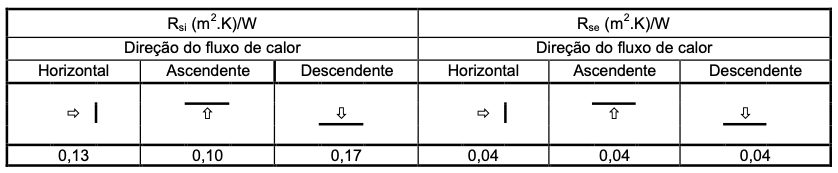
\includegraphics[width=1.0\linewidth]{Tabelas/Req_Interna_NBR15220.png}
    \smallcaption{Fonte:\textcite{abnt15220}}
    \label{tab:Req_NBR15220}
\end{table}

\begin{table}[!htb] 
 \centering
    \caption{Valores médios recomendados para resistência térmica em câmaras de ar não ventiladas, com largura muito maior que a espessura}
    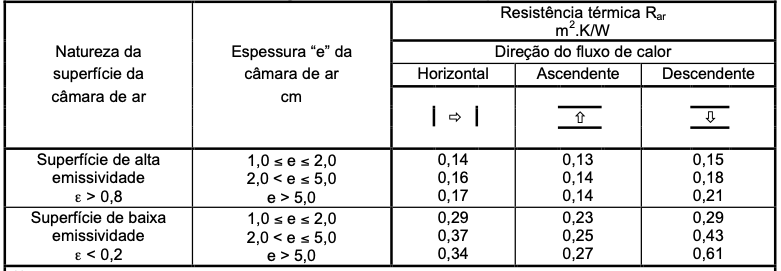
\includegraphics[width=1.0\linewidth]{Tabelas/Req_CamaraAr_NBR15220.png}
    \smallcaption{Fonte:\textcite{abnt15220}}
    \label{tab:Req_Camaras}
\end{table}

\newpage

\section{Balanço de Energia} \label{balenergia}

O balanço de energia representa o comportamento do fluxo de calor em um sistema. Neste contexto, a energia interna ($U$) é a somatória das formas de energia microscópicas de um sistema, sendo representada pelas energias cinética e potencial das moléculas \cite{cengel1998heat}. Vale ressaltar que ao se considerar um regime permanente, a variação da energia ao longo do tempo equivale à zero.

A energia interna está relacionada com as forças intermoleculares que, portanto, unem as moléculas. Assim, a porção cinética de energia refere-se ao calor sensível ao passo que o calor latente está atrelado à mudança de fase. Dessa maneira, observando-se um ambiente climatizado, pode-se afirmar que o calor sensível está relacionado à temperatura enquanto o calor latente à umidade do local.

Considerando-se um sistema de fluxo constante, no qual não ocorre mudanças expressivas nas energias cinética e potencial, e sem a parcela de trabalho, a taxa de transferência de calor sensível ($\dot{Q}_{S}$) sendo adicionado ou retirado de um sistema é representada pela Equação \ref{eq:Qsensível}, na qual $\dot{m}$ representa a vazão mássica, ${Cp}$ é o calor específico do ar à pressão constante, para o qual se considera $1,007 \space kJ/kg K$ à temperatura ambiente, e $\Delta{T}$ equivale à diferença de temperatura.  

\begin{equation} \label{eq:Qsensível}
\begin{aligned}
    \dot{Q}_{S}=\dot{m} \cdot \Delta{h}= \dot{m} \cdot Cp \cdot \Delta{T}
\end{aligned}
\end{equation}

Entretanto, vale ressaltar que a diferença de temperaturas pode ser utilizada apenas para o calor sensível, uma vez que durante a mudança de fase a temperatura permanece constante. Logo, para a análise da taxa de transferência de calor latente ($\dot{Q}_{L}$), pode-se realizar uma comparação da umidade absoluta ($w$) conforme Equação \ref{eq:Qlatente}, na qual $L$ corresponde ao calor latente de vaporização da água.

\begin{equation} \label{eq:Qlatente}
\begin{aligned}
    \dot{Q}_{L}=\dot{m} \cdot \Delta{h}= \dot{m} \cdot L \cdot \Delta{W}
\end{aligned}
\end{equation}

Neste contexto, torna-se importante destacar a influência das pessoas no calor sensível e latente do ambiente. A Tabela \ref{tab:Metabolismo_ashrae} demonstra taxas representativas destas variáveis liberadas pelo ser humano em diferentes níveis de atividade.

\begin{table}[!htb] 
 \centering
    \caption{Taxas Representativas de Calor sensível e Latente Liberados pelo Ser Humano em Diferentes Níveis de Atividade}
    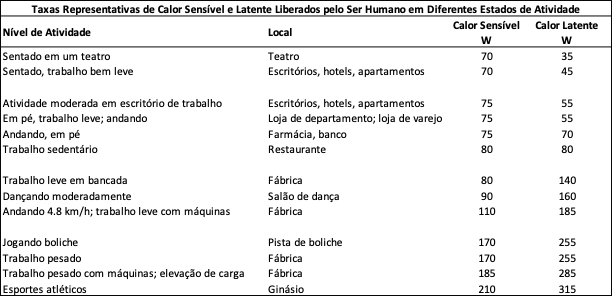
\includegraphics[width=1.0\linewidth]{Tabelas/Metabolismo_ashrae.png}
    \smallcaption{Fonte: Autor. Adaptado de \textcite{handbook2017ashrae}}
    \label{tab:Metabolismo_ashrae}
\end{table}

Outro fator de influência no calor sensível refere-se à iluminação do local. A Tabela \ref{tab:LPD} estabelece valores máximos da densidade de potência da luz, em inglês, \textit{Light Power Density} \textit{(LPD)}, para diferentes locais, representando a carga térmica da iluminação baseada na área atingida pela luz.

\begin{table}[!htb] 
 \centering
    \caption{Densidade de potência da luz para diferentes locais}
    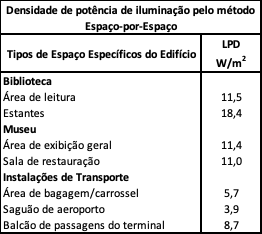
\includegraphics[width=0.6\linewidth]{Tabelas/LPD.png}
    \smallcaption{Fonte: Autor. Adaptado de \textcite{ashrae2013ashrae}}
    \label{tab:LPD}
\end{table}

Além disso, equipamentos presentes no local também contribuem para a carga térmica sensível do sistema. A Tabela \ref{tab:Qs_Monitores} refere-se à influência de monitores no ganho de calor do ambiente.

\begin{table}[!htb] 
 \centering
    \caption{Carga térmica de diferentes monitores}
    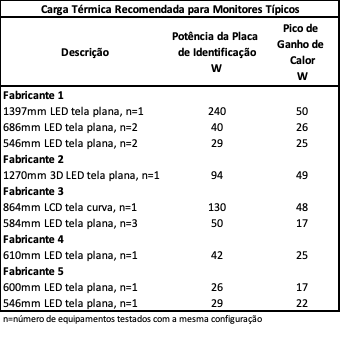
\includegraphics[width=0.6\linewidth]{Tabelas/Qs_Monitores.png}
    \smallcaption{Fonte: Autor. Adaptado de \textcite{sarfraz2018experimental}}
    \label{tab:Qs_Monitores}
\end{table}

Dessa maneira, as fontes de geração ou retirada de calor sensível e latente devem ser somadas a fim de realizar uma análise fundamentada de carga térmica do sistema. 

\section{Ventilação} \label{ventilação}

Por definição ventilação é um processo no qual se retira ou fornece ar por meios mecânicos, de ou para um ambiante fechado, com o objetivo de purificar, controlar a distribuição, a temperatura e a umidade do ar dentro do recinto. Existem dois tipos de ventilação: a Ventilação Geral Diluidora (VGD) e a Ventilação Local Exaustora (VLE). 

\subsection{Ventilação Geral Diluidora} \label{VGD}

A VGD se trata de um sistema para captura do contaminante no ar quando este já não se encontra mais na fonte que o gerou. Segundo \textcite{ventilacaoindustrial} a VGD deve manter o conforto e eficiência do homem, garantir a saúde e segurança do ser humano e conservar em bom estado os equipamentos e materiais utilizados no ambiente.

Uma VGD é composta por um sistema de captação externa, filtro, ventilador de insuflamento, ventilador de exaustão, dutos, bocas de insuflamento e de exaustão e a descarga de ar viciado.

Existem quatro maneiras de instalação e configuração de uma VGD, a depender da situação que o ambiente se encontra. Elas são: insuflamento e exaustão naturais; insuflamento mecânico e exaustão natural; insuflamento natural e exaustão mecânica e insuflamento e exaustão mecânicos \cite{ventilacaoindustrial}.

A VGD tem a função de captar contaminantes no ar para que eles não sejam absorvidos pelo corpo humano. Sabendo disso, existem concentrações adequadas de contaminantes gasosos no ar e elas podem ser calculadas através da Equação \ref{eq:cont}.

\begin{equation} \label{eq:cont}
    \begin{aligned}
C=\frac{n_{Contam.}}{n_{Total}}=\frac{V_{Contam.}}{V_{Total}}
    \end{aligned}
\end{equation}

A ventilação também deverá introduzir uma vazão de ar novo no ambiante, e o fluxo de ar que sai leva embora os contaminantes diluídos. 

Portanto, a  vazão de ar novo é necessária para suprir os níveis de ${O}_{2}$, manter adequado o nível de ${CO}_{2}$ e diluir odores, manter temperatura, e umidade, diluir contaminantes e manter a velocidade do ar confortável. Para isso, existem cálculos, que serão demonstrados mais à frente, para que a vazão de ar novo cumpra todas as necessidades do ambiente.

Para que os níveis de ${O}_{2}$ e ${CO}_{2}$ e odores fiquem aceitáveis, a ANVISA e a ABNT sugerem que a vazão de ar novo mínima necessária siga a Equação \ref{eq:anvisa}, \cite{abnt216401}.

\begin{equation} \label{eq:anvisa}
\begin{aligned}
    \dot{V}_{ArNovo}=N_{Pessoas}\cdot {\dot{V}_{Pessoa}}
\end{aligned}
\end{equation}

Sendo $N_{Pessoas}$ o número de pessoas no ambiente e $\dot{V}_{Pessoas}$ a vazão mínima por pessoa. Sendo esse último valor definido pela ANVISA e é recomendado usar $27$ $m^3/(h\cdot{pessoa}$).

Para que a temperatura seja mantida, a vazão de ar novo a ser colocada no ambiente é descrita nas Equações \ref{eq:tempQ} e \ref{eq:tempV}.

\begin{equation} \label{eq:tempQ}
\begin{aligned}
    \dot{Q}_{S}=\dot{m}_{ArNovo}\cdot {\dot{cp}_{Ar}}\cdot({T_{eq.}-T_{insuf.}})
\end{aligned}
\end{equation}

\begin{equation} \label{eq:tempV}
\begin{aligned}
    \dot{V}_{ArNovo}=\frac{\dot{m}_{ArNovo}}{\rho_{ArNovo}}
\end{aligned}
\end{equation}

Utilizando $\dot{cp}_{ArSeco}=1,006 kJ/(kg\cdot{K})$.

Para manter a umidade no ambiente deve-se colocar ou retirar vapor d'água, e para os cálculos basta tratar como uma troca de calor latente utilizando as Equações \ref{eq:umidQ} e \ref{eq:umidV}.

\begin{equation} \label{eq:umidQ}
\begin{aligned}
    \dot{Q}_{S}=\dot{m}_{ArNovo}\cdot {{L}_{equiv.}}\cdot({\omega_{eq.}-\omega_{insuf.}})
\end{aligned}
\end{equation}

\begin{equation} \label{eq:umidV}
\begin{aligned}
   \dot{V}_{ArNovo}=\frac{\dot{m}_{ArNovo}}{\rho_{ArNovo}}
\end{aligned}
\end{equation}

Onde ${L}_{equiv.}= 2540 kJ/kg$ e $\omega$ é a umidade absoluta.

Os níveis de odores, fumaças e contaminantes precisam ser diluídos e para isso a vazão de ar novo necessária é descrita na Equação \ref{eq:contam.}.

\begin{equation} \label{eq:contam.}
    \begin{aligned}
     \dot{V}_{ArNovo}=\frac{\dot{q}}{C_{Eq.}-C_{Insufl.}}
    \end{aligned}
\end{equation}

Ou quando não se dilui completamente os contaminantes tem-se a Equação \ref{eq:contam.K}.

\begin{equation} \label{eq:contam.K}
    \begin{aligned}
\dot{V}_{\text{ArNovo}} = K \cdot \frac{\dot{q}}{C_{\text{Máx.}} - C_{\text{Insufl.}}}
   \end{aligned}
\end{equation}

$K$ é um coeficiente de segurança que varia de $3$ a $10$.

Manter a velocidade do ar conveniente é importante para o conforto e o ideal é que ela esteja entre $0,1$ $m/s$ e $1,2$ $m/s$. Pode ser medida utilizando a vazão e a área do ambiente, como visto na Equação \ref{eq:veloc}.

\begin{equation} \label{eq:veloc}
\begin{aligned}
   \dot{V}_{ArNovo}=v\cdot{A}
\end{aligned}
\end{equation}

\section{Conforto térmico} \label{confortotermico}

Segundo a \textcite{ASHRAE2009}, conforto térmico é a condição mental que expressa satisfação com o ambiente térmico e é uma avaliação subjetiva. Mas, se 80\% das pessoas de um ambiente estiverem confortáveis, é possível dizer que há conforto térmico.

De acordo com \textcite{konstantinov2015numerical}, o conforto térmico dos passageiros se tornou um critério de design importante para os fabricantes de trens. Isso porque, apesar das sensações individuais serem bem diferentes umas das outras, elas dependem do fluxo de ar, da distribuição de temperatura dentro do ambiente e da radiação de calor na cabine. É por essa questão que o estudo de conforto térmico foca na ventilação e qualidade do ar.

Com base em estudo realizado por \textcite{casellisimulaccao}, um vagão de trem se encontra em diferentes situações em relação à troca de calor do ambiente, portanto, existe um índice que representa um nível aceitável de conforto térmico para as pessoas. Esse índice depende de alguns parâmetros físicos, processos fisiológicos, psicológicos e culturais. 

Em pesquisas anteriores de \textcite{TCCThomas}, tem-se uma análise comparativa do conforto térmico entre as linhas vermelha e azul do Metrô de São Paulo, na qual sensores de temperatura e umidade foram dispostos no interior de um carro da linha vermelha durante o trajeto de ida e volta usualmente percorrido pelo mesmo. Dessa maneira, a coleta de dados ocorreu das 16h08 às 17h29, e foi comparada com simulações realizadas no \textit{software} \textit{Ansys Fluent}, além de avaliar em relação à norma existente \cite{handbook2006american}). Deste modo, foi notada uma influência do fluxo de passageiros na temperatura e umidade no interior dos carros, uma vez que o percurso de retorno, o qual possui maior fluxo de pessoas, apresentou gradiente de temperatura acima do especificado pela norma ao longo de grande parte do trajeto. Além disso, o estudo resultou em uma disparidade de temperatura e velocidade do ar entre a norma e a simulação tanto para os carros da linha azul quanto aos da linha vermelha.

\subsection{Balanço de energia do corpo}

Para que seja possível avaliar o conforto térmico é preciso fazer um balanço de energia baseado na taxa de produção de calor metabólico $(M [W/m^{2}])$ e na taxa de trabalho mecânico realizado $(W [W/m^{2}])$ \cite{ASHRAE2009}. As Equações \ref{eq:energiapessoa} e \ref{eq:energiapessoa1} mostram o balanço de energia.

\begin{equation} \label{eq:energiapessoa}
    \begin{aligned}
    M - W = q_{\text{sk}} + q_{\text{res}} + S
    \end{aligned}
\end{equation}

\begin{equation} \label{eq:energiapessoa1}
    \begin{aligned}
    M - W = (C + R+ E_{\text{sk}}) + (C_{\text{res}} + E_{\text{res}}) + (S_{\text{sk}} + S_{\text{cr}})
    \end{aligned}
\end{equation}

A soma da perda de calor sensível da pele ($(C + R)$ $[W/m^{2}]$) com a taxa total da perda de calor por evaporação da pele ($E_{\text{sk}}$ [$W/m^{2}$]) formam a taxa total de calor perdido da pele($q_{\text{sk}}$ $[W/m^{2}]$). A taxa total de calor perdido pela respiração ($q_{\text{res}}$ $[W/m^{2}]$) se dá pela soma da taxa de calor convectivo perdida pela respiração ($C_{\text{res}}$ $[W/m^{2}]$) e a taxa de calor latente perdido pela respiração ($E_{\text{res}}$ $[W/m^{2}]$). Por fim, a taxa total de armazenamento de calor (S $[W/m^{2}]$) é dada pela soma das taxas de armazenamento de calor na pele ($S_{\text{sk}}$ $[W/m^{2}]$) e de armazenamento de calor nos compartimentos internos do corpo ($S_{\text{cr}}$ $[W/m^{2}]$).


Os parâmetros apresentados nas Equações \ref{eq:energiapessoa} e \ref{eq:energiapessoa1} têm como unidade energia por área superficial do corpo nu (\textcite{ASHRAE2009}). A melhor e mais usual área superficial ($A_{D}$ $[m^{2}]$) utilizada foi elaborada originalmente por \textcite{dubois1916formula} e é mostrada na Equação \ref{eq:dubois}.

\begin{equation} \label{eq:dubois}
    \begin{aligned}
   A_{\text{D}} = 0,202 \cdot m^{0,425} \cdot l^{0,725}
    \end{aligned}
\end{equation}

Onde, $m$ é massa da pessoa em $kg$ e $l$, $a$ altura em $m$. 

As taxas de metabolismo (\textit{M}) tabuladas estão mostradas na Tabela \ref{tab: metabolismo} onde $1$ $met$ equivale à $58,2$ $W/m^2$.

\begin{table}[!htb] 
 \centering
    \caption{Geração de calor metabólico para variadas atividades}
    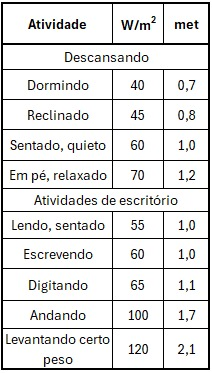
\includegraphics[width=0.4\linewidth]{Tabelas/tabela-met1.jpeg}
    \smallcaption{Fonte: Autor. Adaptado de \textcite{ASHRAE2009}}
    \label{tab: metabolismo}
\end{table}

Porém, para medições mais apuradas do metabolismo pode-se calculá-lo através da Equação \ref{eq:metabolismo}.

\begin{equation} \label{eq:metabolismo}
    \begin{aligned}
   M = \frac{21(0,23RQ + 0,77)Q_{{O_{2}}}}{A_{D}}
    \end{aligned}
\end{equation}

Onde, \textit{M} é a taxa de metabolismo medida em $W/m^2$, \textit{RQ} é o coeficiente respiratório, no qual é razão molar entre a quantidade de ${O}_{2}$ inalado e a quantidade de ${CO}_{2}$ expirado e é adimensional. E, por fim, $Q_{0_{2}}$ é a taxa volumétrica de consumo de oxigênio nas condições de $0^\circ C$ e $101,325$ $kPa$, medida em $mL/s$.

É importante ressaltar que a variável \textit{RQ} depende da atividade da pessoa, sua dieta e sua condição física. Ela pode ser medida calculando o fluxo de ar da expiração e da inspiração da pessoa ou pode ser estimada com certa precisão. Uma boa estimativa para um adulto comum é $RQ$ = $0,83$ para atividades do dia a dia e $RQ$ = $1$ para esforços extremamente pesados.

O oxigênio consumido é estimado através dos batimentos cardíacos e nível de esforço \cite{aastrand2003textbook}. Essas relações estão mostradas na Tabela \ref{tab: bpm e o2}.

\begin{table}[!htb] 
 \centering
    \caption{Batimentos cardíacos e consumo de oxigênio em diferentes níveis de atividade}
    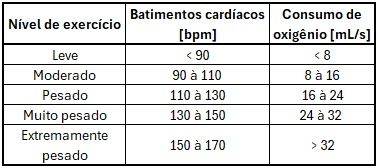
\includegraphics[width=0.5\linewidth]{Tabelas/bpm-o2.jpeg}
    \smallcaption{Fonte: Autor. Adaptado de \textcite{aastrand2003textbook}}
    \label{tab: bpm e o2}
\end{table}

Seguindo a ordem da Equação \ref{eq:energiapessoa}, tem-se a perda de calor sensível pela pele. A troca de calor da pele tem que passar pela roupa para chegar ao ambiente. Esse caminho é feito em série e pode ser descrito em dois passos: o primeiro é da pele, para o isolamento da roupa, para a superfície da roupa, para o ambiente; o segundo é pela superfície da roupa para o ambiente \cite{ASHRAE2009}.

Tanto a convecção (\textit{C}), quanto a radiação (\textit{R}) perdidas pela superfície da roupa do corpo humano podem ser expressas em função do coeficiente de transferência de calor e a diferença de temperatura média da superfície da roupa e a temperatura apropriada do ambiente ao redor, como é visto nas Equações \ref{eq:c} e \ref{eq:r}. 

\begin{equation} \label{eq:c}
    \begin{aligned}
    C = f_{cl} h_{c} (t_{cl} - t_{a})
    \end{aligned}
\end{equation}


\begin{equation} \label{eq:r}
    \begin{aligned}
    R = f_{cl} h_{r} (t_{cl} - t_{r})
    \end{aligned}
\end{equation}

As Equações \ref{eq:c} e \ref{eq:r}, normalmente, são combinadas para expressar a troca de calor sensível total pelos dois mecanismos a partir da temperatura de operação ($t_{o}$). Mostrado na Equação \ref{eq:c+r}.

\begin{equation} \label{eq:c+r}
    \begin{aligned}
    C+R = f_{cl} h_{comb} (t_{cl} - t_{o})
    \end{aligned}
\end{equation}

Onde, $t_{o}$ é calculado pela Equação \ref{eq:to}. E o $h_{comb}$, pela Equação \ref{eq:hcomb}.

\begin{equation} \label{eq:to}
    \begin{aligned}
   t_{o}= \frac{h_{r}t_{r}+h_{c}t_{a}}{h_{r}+h_{c}}
    \end{aligned}
\end{equation}

\begin{equation} \label{eq:hcomb}
    \begin{aligned}
   h_{comb}=h_{r}+h_{c}
    \end{aligned}
\end{equation}

A temperatura de operação ($t_{o}$) é a média ponderada entre a temperatura radiante externa ($t_{r}$) e a temperatura ambiente ($t_{a}$) e seus respectivos coeficientes de transferência de calor. Já a temperatura da superfície da roupa é calculada através de uma iteração, mostrada na Equação \ref{eq:tcl}.

\begin{equation} \label{eq:tcl}
    \begin{aligned}
   t_{cl}= 35,7-0,028(M-W) - R_{cl}(39,6\cdot10^{-9}f_{cl}[(t_{cl}+273)^4-(t_{r}+273)^4]+f_{cl}h_{c}(t_{cl}-t_{a}))
    \end{aligned}
\end{equation}

Segundo a \textcite{ASHRAE2009} ambos os coeficientes $h_{c}$ e $h_{r}$ são calculados para a superfície da roupa. O coeficiente de transferência de calor por convecção é normalmente causado pelo movimento do ar no local ou por movimentos dos corpos. As equações que estimam $h_{c}$ estão apresentadas na Tabela \ref{tab: valores de hc}. 

\begin{table}[!htb] 
 \centering
    \caption{Equações para estimativa do coeficiente de transferência de calor por convecção}
    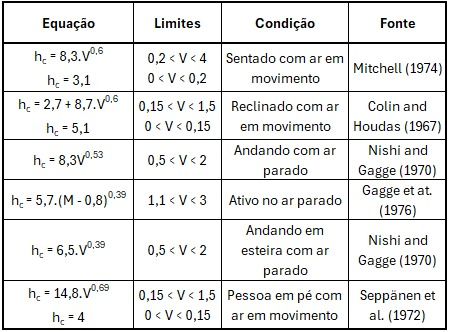
\includegraphics[width=0.5\linewidth]{Tabelas/tabela-hc.jpeg}
    \smallcaption{Fonte: Autor. Adaptado de \textcite{ASHRAE2009}}
    \label{tab: valores de hc}
\end{table}


Já o coeficiente de transferência de calor por radiação é calculado através da Equação \ref{eq:hr}.

\begin{equation} \label{eq:hr}
    \begin{aligned}
   h_{r}=4 \epsilon \sigma \frac{A_{r}}{A_{D}}(273,2 + \frac{t_{cl}+t_{r}}{2})^3
    \end{aligned}
\end{equation}

Na qual, $\epsilon$ é a emissividade, normalmente usada 0,95 para a pele humana, $\sigma$ é a constante de Stefan-Boltzmann ($5,67\cdot10^{-8}$ $W/m^{2}K^{4}$) e $A_{r}$ é a área de radiação efetiva do corpo ($m^2$). A razão $A_{r}/A_{D}$ é 0,70 para uma pessoa sentada e 0,73 para uma pessoa em pé.

Em alguns casos, a variável $t_{cl}$ é desconhecida, portanto não é possível calcular o $h_{r}$. Para isso, em temperatura típicas de ambientes internos $h_{r}$ é quase constante, podendo, assim, ser usada a aproximação vista na Equação \ref{eq:hr1}.

\begin{equation} \label{eq:hr1}
    \begin{aligned}
   h_{r}=4,7\cdot \epsilon
    \end{aligned}
\end{equation}


Um fator de correção $f_{\text{cl}}$ deve ser aplicado para que a transferência de calor da pele leve em consideração a área superficial do corpo com a resistência da superficial da roupa ($I_{cl}$). A Tabela \ref{tab: valores de fcl e icl} mostra alguns valores para variados conjuntos de roupas \cite{mccullough1989data}.

\begin{table}[!htb] 
 \centering
    \caption{Valores de isolamento e permeabilidade para conjuntos de roupas típicos}
    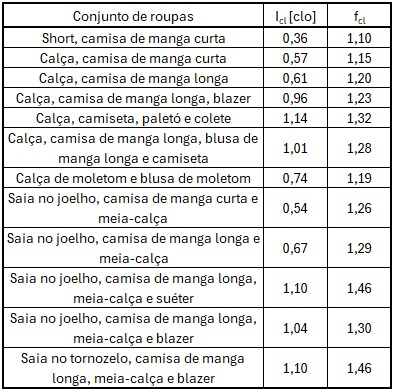
\includegraphics[width=0.5\linewidth]{Tabelas/tabela-roupas.jpeg}
    \smallcaption{Fonte: Autor. Adaptado de \textcite{mccullough1989data}}
    \label{tab: valores de fcl e icl}
\end{table}

Na Tabela, $I_{cl}$ está em unidade de $clo$ que corresponde à $0,155$ $m^2K/W$. Para não haver confusão quando a resistência da roupa for utilizada em $m^2K/W$ o símbolo $R_{cl}$ será usado.

Em casos em que se pode medir $f_{cl}$ e as condições são bem definidas é possível calcular $R_{cl}$ através da Equação \ref{eq:rcl}.

\begin{equation} \label{eq:rcl}
    \begin{aligned}
   R_{cl}= \frac{t_{sk}-t_{o}}{q}-\frac{1}{h\cdot f_{cl}}
    \end{aligned}
\end{equation}

Onde \textit{q} é o calor perdido do corpo em $W/m^2$ e $t_{sk}$ é a temperatura média do compartimento da pele e pode ser descrita pela Equação \ref{eq:tsk}.

\begin{equation} \label{eq:tsk}
    \begin{aligned}
   t_{sk}= 35,7 - 0,00275(M-W)
    \end{aligned}
\end{equation}

Ainda sobre a perda de calor da pele para o ambiente tem-se o calor perdido por evaporação ($E_{sk}$), mostrado na Equação \ref{eq:esk}.

\begin{equation} \label{eq:esk}
    \begin{aligned}
   E_{sk}= \frac{w(p_{sk,s}-p_{a})}{R_{e,cl}+\frac{1}{f_{cl}h_{e}}}
    \end{aligned}
\end{equation}

Na Equação \ref{eq:esk} tem-se a presença de duas pressões: a pressão de vapor d'água na pele, na temperatura $t_{sk}$ (normalmente assumido como saturado) ($p_{sk,s}$ [$kPa$]) e a pressão de vapor d'água no ambiente ($p_{a}$ [$kPa$]). Tem-se também a resistência de transferência de calor por evaporação da roupa ($R_{e,cl}$ [$m^2kPa/W$]), equivalente ao $R_{cl}$, a umidade da pele ($w$) e o coeficiente de transferência de calor por evaporação ($h_{e}$ [$W/m^2K$]).

A umidade da pele ($w$) é dada pela razão da verdadeira perda de calor por evaporação pela perda máxima de calor na qual ocorre em $E_{max}$ onde o calor perdido é máxima quando $w$ = $1$. Ela é muita relacionada com o desconforto térmico e é um ótimo medidor se as temperaturas estão muito altas. Teoricamente, a umidade da pele pode se aproximar de 1 enquanto o corpo se mantém controlado termicamente \cite{berglund1977evaporation}. \textcite{azer1982design} recomenda um valor de 0,5 para condições de pessoa saudável em um ambiente climatizado.

Com isso, tem-se a primeira parcela da equação de energia (Equação \ref{eq:energiapessoa1}), a perda total de calor pela pele ($q_{sk}$). Essa parcela pode ser escrita, também, como mostra a Equação \ref{eq:qsk}.

\begin{equation} \label{eq:qsk}
    \begin{aligned}
   q_{sk}= (C + R + E_{sk})
    \end{aligned}
\end{equation}

Após descrita a parcela da perda total de calor pela pele, tem-se a parcela de perda de calor pela respiração. Essa parcela é mostrada na Equação \ref{eq:qres}.

\begin{equation} \label{eq:qres}
    \begin{aligned}
   q_{res}= (C_{res} + R_{res})
    \end{aligned}
\end{equation}

A perda total de calor pela respiração, normalmente é expressada em função de calores sensível ($C_{res}$) e latente ($E_{res}$). As Equações \ref{eq:cres} e \ref{eq:eres} são aproximações simplificadas das expressões de perdas de calor, pois a perda de calor pela respiração seca é relativamente pequena. Portanto, as equações serão utilizadas em condições normais de temperatura e umidade ($20^\circ C$ e $50\%$, respectivamente) \cite{ASHRAE2009}.

\begin{equation} \label{eq:cres}
    \begin{aligned}
   C_{res}= 0,0014M(34-t_{a})
    \end{aligned}
\end{equation}

\begin{equation} \label{eq:eres}
    \begin{aligned}
   R_{res}= 0,0173M(5,87-p_{a})
    \end{aligned}
\end{equation}

A última parcela necessária para que o balanço de energia possa ser calculado é a taxa de armazenamento de calor do corpo. Essa taxa é dividida em duas partes: a primeira é a taxa de armazenamento de calor na pele, e a segunda, a taxa de armazenamento de calor nos compartimentos internos do corpo. A taxa de armazenamento pode ser escrita separadamente para cada compartimento em termos de capacidade térmica e tempo de troca de temperatura em cada compartimento. \cite{ASHRAE2009} As Equações \ref{eq:scr} e \ref{eq:ssk}, mostram as formulações das taxas. 

\begin{equation} \label{eq:scr}
    \begin{aligned}
   S_{cr}= \frac{(1-\alpha_{sk})mc_{p,b}}{A_{D}}\cdot \frac{dt_{cr}}{d\theta}
    \end{aligned}
\end{equation}

\begin{equation} \label{eq:ssk}
    \begin{aligned}
   S_{sk}= \frac{\alpha_{sk}mc_{p,b}}{A_{D}}\cdot \frac{dt_{sk}}{d\theta} 
    \end{aligned}
\end{equation}

A variável $\alpha_{sk}$ é a fração mássica do corpo concentrada no compartimento da pele (adimensional); $c_{p,b}$ é a capacidade térmica específica do corpo ($3490$ $J/(kgK)$); as temperaturas $t_{cr}$ e $t_{sk}$ são, respectivamente, a temperatura do compartimento central e da pele ($\circ C$); $\theta$ é o tempo, em segundos.

A fração mássica do corpo ($\alpha_{sk}$) pode ser calculada por meio da Equação \ref{eq:alpha} e depende do fluxo sanguíneo na superfície da pele, $\dot{Q}_{bl}$ ($L/hm^2$), mostrada na Equação \ref{eq:qbl}.  

\begin{equation} \label{eq:alpha}
    \begin{aligned}
    \alpha_{sk}= 0,0418+ \frac{0,745}{\dot{Q}_{bl} - 0,585} 
    \end{aligned}
\end{equation}

\begin{equation} \label{eq:qbl}
    \begin{aligned}
   \dot{Q}_{bl}= \frac{BFN + c_{dil}(t_{cr-37})}{1 + S_{tr}(34-t_{sk})} 
    \end{aligned}
\end{equation}

Para uma pessoa comum os parâmetros $BFN$, $c_{dil}$ e $S_{tr}$ têm valores de $6,3$, $50$ e $0,5$, respectivamente. Um ser humano tem um $\dot{Q}_{bl}$ limitado a um máximo de $90$ $L/(hm^2)$. 

\subsection{\textit{Predicted Mean Vote (PMV)} e \textit{Predicted Percent of Dissatisfied (PPD)}}

Apesar do conforto térmico ser subjetivo é possível avaliá-lo através do método \textit{PMV} - \textit{PPD}, criado por \textcite{fanger1970thermal} para prever o voto de satisfação das pessoas e a porcentagem de pessoas insatisfeitas com o ambiente. \textcite{fanger1970thermal}, relacionou o \textit{PMV} com o balanço entre o verdadeiro fluxo de calor do corpo em um determinado ambiente e o fluxo de calor necessário para se atingir o conforto térmico, comparando-os com a escala de conforto térmico da \textcite{ASHRAE2009}, vista na Tabela \ref{tab: conforto} através da Equação \ref{eq:pmv}.

\begin{table}[!htb] 
 \centering
    \caption{Escala de conforto térmico }
    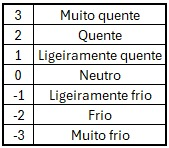
\includegraphics[width=0.3\linewidth]{Tabelas/nivel-conforto.jpeg}
    \smallcaption{Fonte: Autor. Adaptado de \textcite{mccullough1989data}}
    \label{tab: conforto}
\end{table}

\begin{equation} \label{eq:pmv} 
    \begin{aligned}
   PMV = [0,303 \cdot e^{-0,036\cdot M}+0,028]\cdot ((M-W)-3,05\cdot10^{-3}\cdot [5733-6,99\cdot(M-W)-p_{a}]\\
   -0,42\cdot[(M-W)-58,15]-1,7\cdot 10^{-5}\cdot M \cdot(5867-p_{a})-0,0014\cdot M\cdot(34-t_{a})\\
   -3,96\cdot10^{-8}\cdot f_{cl}\cdot[(t_{cl}+273)^4-(t_{r}+273)^4]-f_{cl}\cdot h_{c}\cdot(t_{cl}-t_{a}))
    \end{aligned}
\end{equation}

A equação pode ser reescrita como a Equação \ref{eq:pmvl}. Onde $L$ é a carga térmica total do corpo.

\begin{equation} \label{eq:pmvl}
    \begin{aligned}
   PMV = [0,303 \cdot e^{-0,036\cdot M}+0,028]\cdot L
    \end{aligned}
\end{equation}

Depois de estimado o voto é possível estimar a insatisfação de conforto por meio da Equação \ref{eq:ppd}.

\begin{equation} \label{eq:ppd}
    \begin{aligned}
   PPD = 100 - 95\cdot e^{-(0,03353 PMV^4 + 0,2179PMV^2)}
    \end{aligned}
\end{equation}

Ao relacionar o \textit{PMV} com o \textit{PPD} tem-se o gráfico mostrado na Figura \ref{fig:graficopmvppd}.

\begin{figure}[!htp] 
 \centering
    \caption{Gráfico \textit{PMV} x \textit{PPD}}
    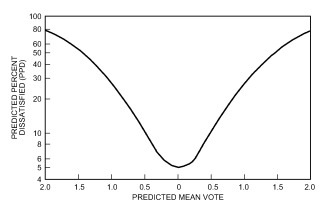
\includegraphics[width=0.6\linewidth]{Imagens/grafico-pmv-ppd.jpeg}
    \smallcaption{Fonte: \textcite{fanger1970thermal}}
    \label{fig:graficopmvppd}
\end{figure}

\section{\textit{Computational Fluid Dynamics} (\textit{CFD})}

Fluxos e fenômenos relacionados podem ser descritos a partir de equações parciais diferenciais, as quais, usualmente, não podem ser resolvidas analíticamente. Dessa maneira, o método da discretização permite aproximar tais equações a um sistema algébrico que possa ser solucionado por meios computacionais. Assim, as aproximações são aplicadas a pequenos domínios de espaço e tempo \cite{peric2002computational} para simular o fenômeno em um determinado período e, portanto, quanto menor a malha utilizada, isto é, quanto menor o domínio de espaço e tempo adotado, maior a precisão dos resultados, embora exija maior capacidade computacional. Assim, a análise numérica dos escoamentos é denominada Dinâmica dos Fluidos Computacional que, em inglês, é representada pela sigla \textit{CFD}. 

Em estudos de conforto térmico a dinâmica dos fluidos computacional é muito utilizada por ser uma ferramenta que consegue simular de maneira muito exata as condições térmicas do ambiente.   

Como um exemplo de estudo de conforto térmico por \textit{CFD} é possível citar o estudo realizado por \textcite{li2019multi}. Este artigo tinha como objetivo estudar o conforto térmico dentro do carro de um trem de alta velocidade (\textit{HST}) chinês, por meio de simulações \textit{CFD} e posteriormente utilizar a krigagem (ou \textit{Kriging}, em inglês), para substituir a simulação por dinâmica dos fluidos computacional, por ser mais rápida e otimizada. Para chegar em resultados confiáveis e com o mínimo de erros computacionais possíveis, o estudo de \textcite{li2019multi} realizou 25 simulações, no \textit{software}, com parâmetros diferentes mas com as mesmas resoluções de malha e condições de contorno. Com os resultados das simulações, foi possível obter parâmetros como temperatura da cabine do carro, concentração de contaminantes e o \textit{PMV} (\textit{Predicted mean vote}) que é um modelo desenvolvido por \textcite{fanger1970thermal}, muito utilizado em estudos de conforto térmico, no qual se utiliza a temperatura da pele para definir o conforto.

\chapter{Materiais e Métodos}

\section{Metodologia}

O objeto deste estudo é a análise de um dos carros da frota L da linha 1 - Azul, do Metrô de São Paulo. Esta frota é uma atualização da antiga frota  D, de 1986, e foi inaugurada em 2011, sendo sua última modernização em 2017. Um carro desta frota e o mapa da rede do metrô e trem de São Paulo são mostrados nas Figuras \ref{fig:Trem_da_Frota_L} e \ref{fig:mapa-da-rede-metro-0124-abre}. Por motivos de sigilo e segurança, os tamanhos reais e as plantas do metrô não poderão ser mostradas, nem divulgadas.

\begin{figure}[!htb]
    \centering
    \begin{minipage}{0.45\textwidth}
        \caption{Trem da frota L do Metrô de São Paulo}
        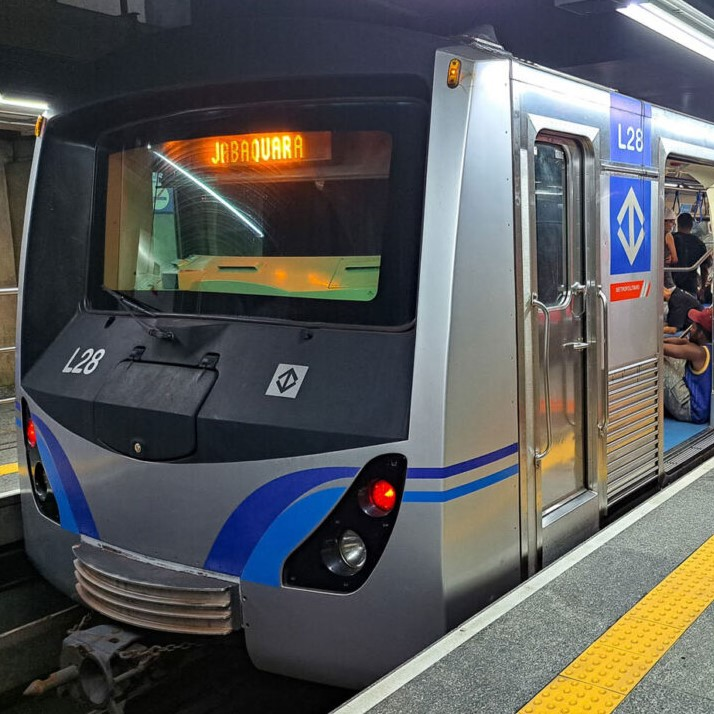
\includegraphics[width=\linewidth, height=6cm]{Imagens/Alstom_L28.jpg}
        \smallcaption{Fonte: \textcite{FrotaL}}
        \label{fig:Trem_da_Frota_L}
    \end{minipage}\hfill
    \begin{minipage}{0.45\textwidth}
        \caption{Mapa da rede de trem e metrô da cidade de São Paulo}
        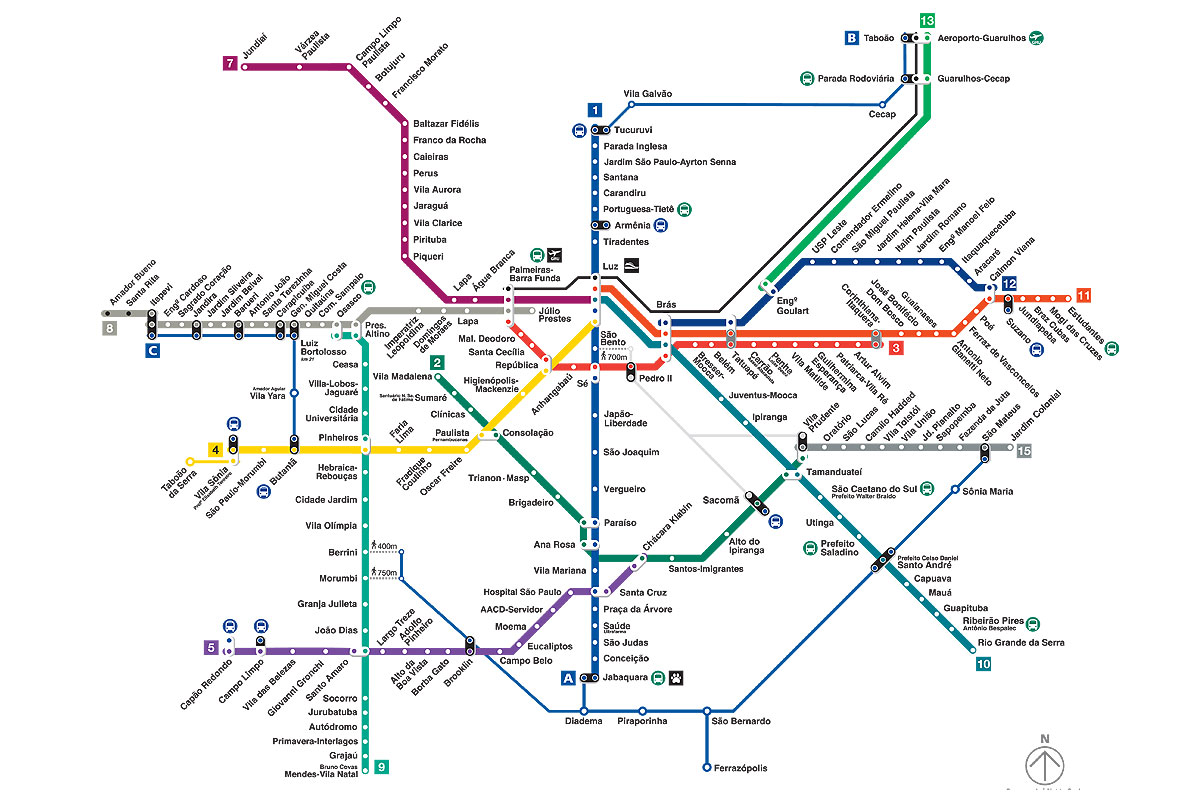
\includegraphics[width=\linewidth, height=6cm]{Imagens/mapa-da-rede-metro-0124-abre.jpg}
        \smallcaption{Fonte: \textcite{Mapametro}}
        \label{fig:mapa-da-rede-metro-0124-abre}
    \end{minipage}
\end{figure}


Será feita a pesquisa da análise dos parâmetros de conforto térmico, levando em conta as normas vigentes. Após a conclusão da pesquisa e das revisões bibliográficas, serão realizadas reuniões pontuais com a equipe do Metrô de São Paulo, nas quais as ideias do grupo serão alinhadas e discutidas com a empresa. 

A seguir, será efetuada a escolha dos melhores sensores considerando o custo benefício e aplicação específica empregada. Para validar o funcionamento de todos os sensores e o código desenvolvido, serão realizados testes iniciais utilizando uma \textit{protoboard}, garantido assim o funcionamento de todos os componentes em conjunto, podendo-se assim seguir para próxima parte que será o desenvolvimento de quatro \textit{Printed Circuit Boards} (\textit{PCB}), com todos os componentes já integrados. 

Serão implementadas três placas iguais com o intuito de permanecer dentro do vagão do Metrô medindo as informações de conforto térmico, realizando a medição das informações em três locais estratégicos. O primeiro na altura das pessoas na extremidade do carro, a segunda no ponto de exaustão bem no nível e a última localizada no centro do carro na altura no insuflamento. sendo possível assim estimar uma média do local, considerando uma simetria do vagão. A ultima e quarta placa será para medição da pressão do local, para ser possível converter os dados relativos em absolutos, e se localizará ao lado da primeira placa de conforto térmico. É possível observar tudo oque foi descrito na Figura \ref{fig:metodo_de_medicao}.

\begin{figure}[!htb]
 \centering
    \caption{Explicação da instalação das placas de medições}
    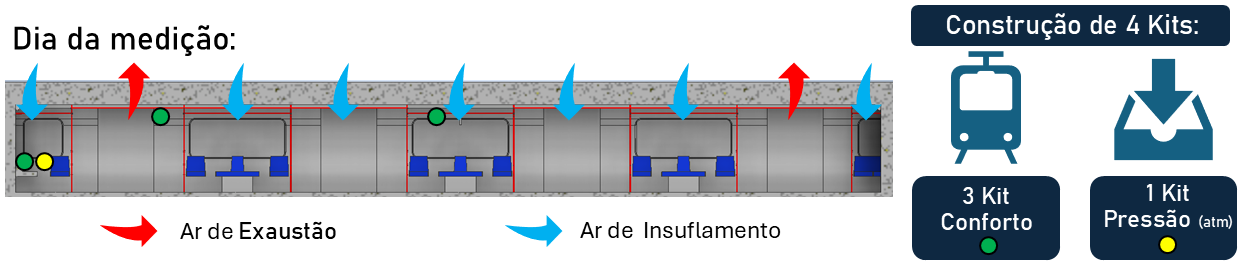
\includegraphics[width=1\linewidth]{Imagens/metodo_de_medicao.png}
    \smallcaption{Fonte: Autor}
    \label{fig:metodo_de_medicao}
\end{figure}


Vale ressaltar que a partir de uma conversa com o Metrô de São Paulo, foi sugerido a presença de um membro do grupo para cuidar de cada \textit{PCB}, sendo assim será realizado a medição em diferentes horários com o intuito de entender oque ocorre em momentos com fluxo menor e momentos com maior fluxo de pessoas.

Sucessivamente, com posse dos dados obtidos pelos sensores e os disponibilizados pelo Metrô de São Paulo, será realizado o tratamento dos mesmos em um software dedicado e serão elaboradas as primeiras análises do comportamento que o ar possui no carro, e serão criadas as primeiras correlações. Simultaneamente serão elaborados os cálculos de \textit{PMV} e \textit{PPD} e das normas ABNT e \textit{ASHRAE}, além de todos cálculos termodinâmicos assim podendo ter um comparativo com o teórico e o valor esperado pelas normas.

Posteriormente, utilizando o que há de mais moderno, a análise computacional a partir do \textit{CFD}, serão gerados novos dados complementares aos instrumentais, levando como base as plantas de ventilação e de projeto disponibilizados pelo Metrô de São Paulo.

Ao final, a comparação dos dados obtidos pela instrumentação com os dados da análise do \textit{CFD} e o esperado pela teoria e as normas dará a robustez suficiente para uma conclusão objetiva do que o Metrô de São Paulo está fazendo e elaboração de possíveis propostas de melhorias poderia melhorar. Com isso tem-se o fluxograma que resume a metodologia do trabalho, esquematizado na Figura \ref{fig: Fluxograma}.

\begin{figure}[!htb] 
 \centering
    \caption{Fluxograma da metodologia}
    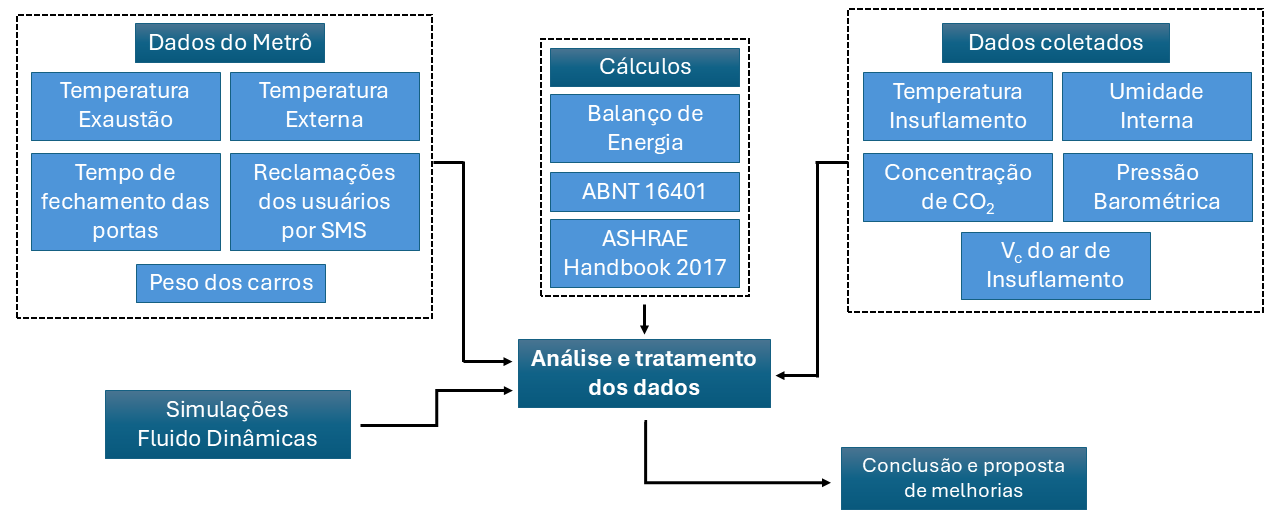
\includegraphics[width=1\linewidth]{Imagens/Fluxograma_da_metodologia.png}
    \smallcaption{Fonte: Autor}
    \label{fig: Fluxograma}
\end{figure}


\section{Premissas do Projeto e Parâmetros das Normas} \label{premissas}

As normas são fundamentais a fim de definir os parâmetros e condições do ambiente que propiciem conforto térmico às pessoas presentes em um determinado local.

De acordo com a norma \textcite{abnt216401}, os parâmetros que influenciam na sensação de conforto térmico são: temperatura operativa, velocidade do ar e umidade relativa do ar. Assim, fatores como o tipo de roupa e nível de atividade física das pessoas podem interferir nestes parâmetros e, portanto, os intervalos de valores recomendados visam proporcionar a sensação de conforto térmico para, no mínimo, 80\% das pessoas.

A norma utilizada para o cálculo do conforto térmico foi o capítulo 9 da \textcite{ASHRAE2009} que descreve todo o processo de balanço de energia do corpo humano e conforto térmico, bem como a escala de sensação térmica que é muito utilizada para a comparação do ambiente com a norma. 

Zonas de conforto foram determinadas pela \textit{ASHRAE} conforme a Figura \ref{fig: Zonas_Conforto}. Assim, baseando-se nestes parâmetros, a norma \textcite{abnt216401} estipula valores adequados de temperatura operativa, umidade relativa e velocidade do ar para o verão e inverno, os quais podem ser observados na Tabela \ref{tab: Parâmetros Ar}. 

\begin{figure}[!htb] 
 \centering
    \caption{Zonas de Conforto conforme \textit{ASHRAE}}
    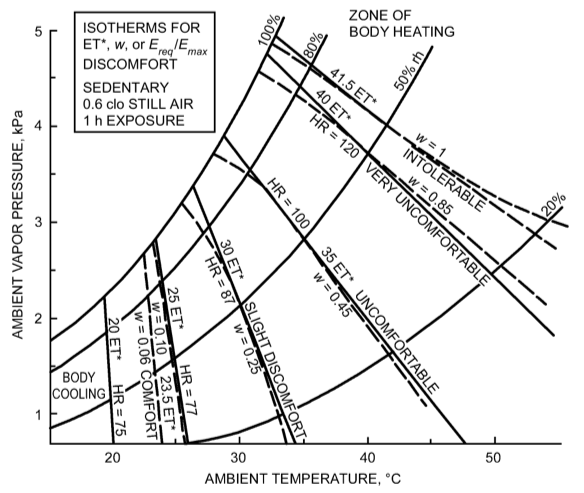
\includegraphics[width=0.8\linewidth]{Imagens/Zonas_Conforto.png}
    \smallcaption{Fonte: \textcite{ashrae2005ashrae}}
    \label{fig: Zonas_Conforto}
\end{figure}

\begin{table}[!htb] 
 \centering
    \caption{Parâmetros adequados para o ar nas condições de verão e inverno}
    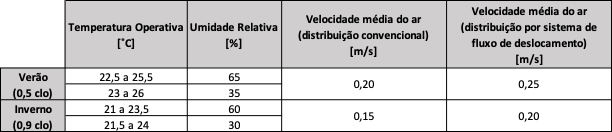
\includegraphics[width=1.0\linewidth]{Tabelas/Tabela_ABNT.png}
    \smallcaption{Fonte: Autor. Adaptado de \textcite{abnt216401}}
    \label{tab: Parâmetros Ar}
\end{table}

Outro ponto importante está ligado à quantidade de ${CO}_{2}$ que será considerada como aceitável nesta análise. O dióxido de carbono é um dos gases do efeito estufa mais encontrados na atmosfera, visto que é exalado por todo ser humano, ao passo que é possível afirmar que o dobro de pessoas geram o dobro da quantidade de ${CO}_{2}$ \cite{ashrae2001}, que geralmente, como também é o caso deste estudo, é analisada em partes por milhão (\textit{ppm}). Este gás costuma ser encontrado em valores entre os $400$ e $1000$ \textit{ppm} para áreas internas, mas pode margear os $2500$ \textit{ppm}, dadas certas situações, sendo que acaba não por ser um agente tóxico, mas sim um asfixiante simples, pois toma o lugar do oxigênio no corpo humano, entretanto problemas reais de respiração e no sistema nervoso só ocorrem em concentrações a partir dos trinta e cinco mil \textit{ppm} \cite{handbook2017ashrae}. O mesmo artigo cita também um valor limítrofe para um dia de 8 horas de trabalho, sendo este o de $5000$ \textit{ppm}, mas é importante lembrar que no caso desta análise, onde não há fontes mais significativas de ${CO}_{2}$ além dos usuários do Metrô, é essencialmente impossível alcançar esta marca.

De modo a estabelecer parâmetros voltados a segurança nestes ambientes internos, a \textcite{abnt17037} apresentou a norma ABNT NBR 17037, que define um ponto saudável para a concentração de dióxido de carbono em $700$ \textit{ppm} acima da medida encontrada em área externa, substituindo portanto a resolução nº9/2003 da ANVISA, que afirmava um valor máximo de $1000$ \textit{ppm} independente do ar externo. A resolução antiga considerava um valor de ${CO}_{2}$ externo de $300$ \textit{ppm}, que somada aos $700$ \textit{ppm} resulta no valor apresentado, mas visto que as taxas deste gás vem subindo a cada ano, é necessário ajustar o máximo esperado. Estudos como o de \textcite{stoco} revelam ainda valores úteis para este estudo, já que o autor registrou aferições médias de $430,9$ $\pm$ $23,3$ \textit{ppm} do contaminante efetuadas no Instituto de Astronomia, Geofísica e Ciências Atmosféricas da USP, situado no Butantã.

Dados os apontamentos citados, é também relevante citar que recentes estudos apresentam inconsistências quanto ao efeito do dióxido de carbono sobre o comportamento humano, mas um ponto em comum é que a partir dos $1000$ \textit{ppm} há reduções na capacidade cognitiva do indivíduo \cite{astmD6245}, junto à sensação de fadiga, que aumenta conforme as concentrações deste gás sobem. Este fato explica o motivo por trás dos limites recomendados pela ABNT NBR 17037 e a resolução nº9/2003, já que, apesar da mudança entre normas, o resultado é relativamente próximo ao se considerar que a concentração externa varia de $300$ a $500$ \textit{ppm} \cite{ashrae2016}. %imagem com efeitos co2 ppm

Dados estes apontamentos, a questão da 

\subsection{Hipóteses simplificadoras do trabalho} \label{simplificação}

Para os cálculos de conforto foi necessário fazer algumas simplificações porque certos parâmetros não podem ser medidos sem um estudo mais aprofundado, o que foge do escopo deste trabalho. 

Inicialmente, as pessoas foram consideradas como sendo paralelepípedos de base quadrada com altura de $1,7 m$ e com $70 kg$ de peso, sendo uma boa estimativa para a população masculina brasileira, para os cálculos de metabolismo e área superficial do corpo.

Em relação à situação das pessoas dentro do metrô, foi considerado que o nível de atividade exercida dentro dos vagões do metrô foi leve ou sedentário com batimentos cardíacos menores que $90 bpm$ e, portanto, o consumo de oxigênio ($\dot{Q}_{O_{s}}$) foi de $8 mL/s$ e o $RQ$ foi constante em $0,83$. Também foram consideradas que estavam sentadas com o ar parado, ocasionando em um coeficiente de troca de calor convectivo ($h_{c}$) constante de $3,1 W/m^2K$ e utilizando shorts e camiseta de manga curta, por isso os índices $I_{cl}$ e $f_{cl}$ foram de $0,57$ e $1,15$, respectivamente. Vale lembrar que a pressão de vapor d'água é tabelada e varia de acordo com a $t_{a}$, mas para simplificação de cálculos foi usado o valor de $2653 Pa$.

A temperatura radiante média ($t_{r}$) foi considerada igual a temperatura ambiente ($t_{a}$), porque para medi-la seria necessário medidas mais específicas.  Também foi considerado para efeito de contas que a temperatura do salão do metrô (temperatura ambiente) é igual a temperatura de exaustão.
   
Considerou-se que o vagão não possui entradas de ar externo por meio de frestas e, portanto, a carga térmica desta fonte foi desprezada. Além disso para facilitar a análise da carga térmica, considerou-se como zero a variação da energia interna ao longo do tempo, isto é, a situação foi analisada como em regime permanente.

Sobre a questão dos parâmetros de dióxido de carbono (${CO}_{2}$), foi também realizada uma simplificação para a posterior análise de seus níveis no vagão. Idealmente, deveriam ser realizadas medições dos níveis de ${CO}_{2}$ externos ao carro em conjunto com o sensoriamento interno. Entretanto, após diálogos com a equipe do Metrô, revelou-se que um kit externo ocasionaria alguns problemas, dadas as limitações dos possíveis locais de fixação do mesmo. Assim, tomando como base os apontamentos da seção \ref{premissas}, ao adicionar os níveis externos do gás, que variam de $300$ a $500$ partes por milhão, aos $700$ \textit{ppm} recomendados pela ABNT NBR 17037, são evidenciados valores de $1000$ a $1200$ \textit{ppm} como os limites ideais. 

Entretanto, deve também levar-se em consideração as características do sistema de ar das estações e tuneis por onde passa a linha azul. Apesar de, em sua maioria, serem presentes as estações e tuneis subterrâneos, há também uma grande quantidade de momentos onde o Metrô passa por áreas abertas, além de que a ventilação observada nos pontos subterrâneos funciona de maneira muito eficiente, renovando constantemente o ar que passa por lá. Deste modo, o grupo está considerando esta área majoritariamente interna como  tendo as propriedades de uma área externa, e com isso foi selecionada para este estudo uma concentração de $500$ \textit{ppm} de ${CO}_{2}$ como base do ar externo, já que este é o limite superior do que se pode considerar. Com estes fatos e a norma em mente, o limite saudável da concentração de dióxido de carbono estabelecido para esta análise fica situado em $1200$ \textit{ppm}.

\subsection{Parâmetros estabelecidos pelo Metrô de São Paulo}

O \textcite{metrosp2024} possui seu próprios parâmetros para avaliação da temperatura, pois o sistema de ar-condicionado não possui nenhum sensor de insuflamento, apenas de exaustão. Logo, para saber a temperatura esperada que estará no ambiente antes de voltar para o insuflamento, o Metrô criou uma métrica empírica própria que é definida pela Equação \ref{eq:temperatura_metro}, que é uma equação linear com seus termos compostos por $T_{ic}$, temperatura interna esperada que o carro tenha, logo a temperatura que o ar-condicionado tenta manter o vagão, $T_{adj}$, é uma temperatura de ajuste, também chamada de \textit{set-point}, sendo possível alterá-la entre ${21}^\circ C$ a ${25}^\circ C$, a $T_{ext}$, que é temperatura externa no momento. O \textcite{metrosp2024} utiliza essa forma por ser algo mais fluido que a normas padrões para ar-condicionados oque previne o choque térmico dos passageiros antes de entrar nos vagões.

\begin{equation} \label{eq:temperatura_metro}
\begin{aligned}
{T}_{ic} = {T}_{adj} \cdot {0,25} \cdot ({T}_{ext} - {19})
\end{aligned}
\end{equation}

Essas relações de valores de temperatura são representadas em um gráfico mostrado na Figura \ref{fig:temperatura_metro}, com a $T_{adj}$ variando de ${21}^\circ C$, ${23}^\circ C$ e ${25}^\circ C$. O \textcite{metrosp2024}, até o momento deste trabalho, tem como $T_{adj}$ definida em  ${23}^\circ C$. A temperatura $T_{ic}$ temperatura desejada pode variar em ${2}^\circ C$ para mais ou para menos, sendo usada como parâmetro para o trabalho.

\begin{figure}[!htb]
\centering
    \caption{Relação de temperaturas para o Metrô de São Paulo}
    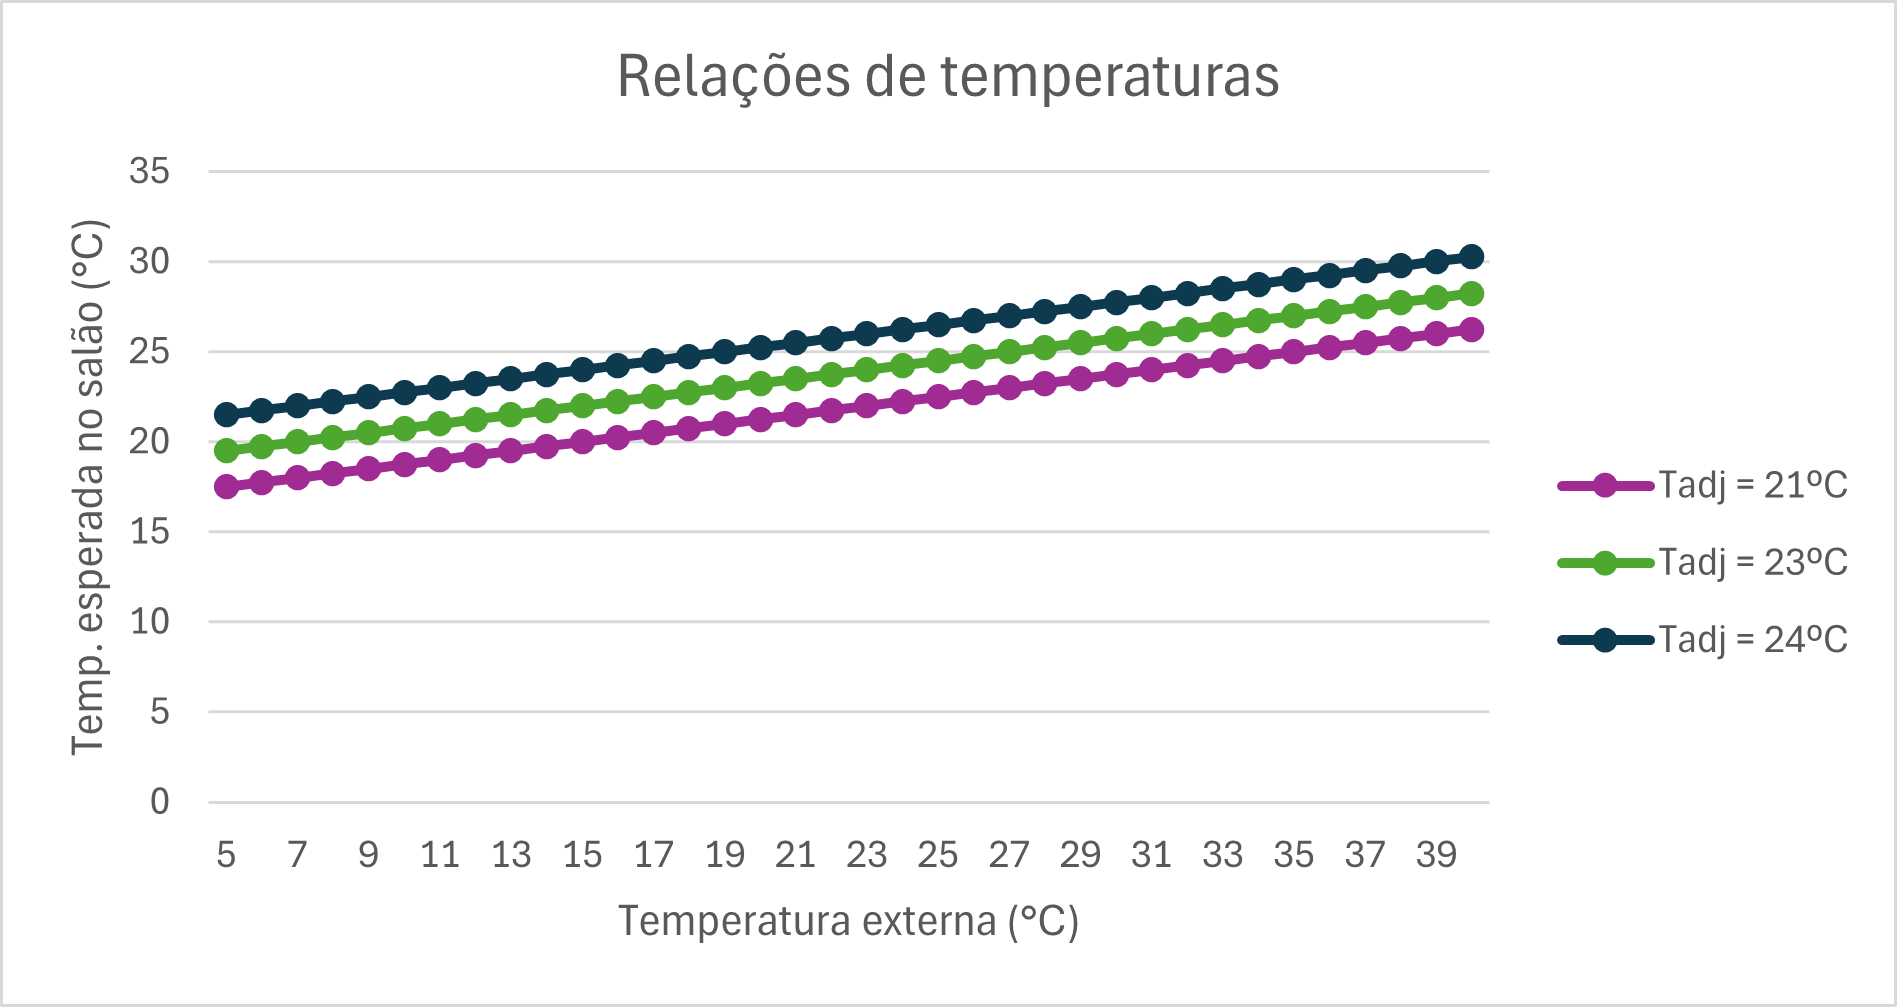
\includegraphics[width=0.8\linewidth]{Imagens/Relacoes_de_temperaturas.png}
    \smallcaption{Fonte:\textcite{metrosp2024}}
    \label{fig:temperatura_metro}
\end{figure}

Outro parâmetro importante de ser analisado é o número de pessoas no vagão, que o Metrô de São Paulo também possui uma métrica própria, considerando a área total disponível de 46 $m^2$ e 48 cadeiras úteis, existe dois tipos de carregamento um com o total de ${6}$ $passageiros/m^2$ que equivale a 228 em pé e 48 sentadas de ${8}$ $passageiros/m^2$ que equivale a 320 em pé e 48 sentadas. Para o estudo o \textcite{metrosp2024} informou para adotar o segundo tipo de carregamento.  

\section{Sistema de aquisição de dados}

A aquisição de dados é parte fundamental do trabalho, sendo a base para futuras análises e correlações. Como descrito na seção \ref{confortotermico}, certos parâmetros como temperatura, umidade e a qualidade do ar interferem diretamente na percepção do que é agradável ou não para as pessoas. Logo é necessário uma robustez dos dados que serão coletados e aferidos.

Parte dos dados apresenta carácter quantitativo, como a temperatura do ar de insuflamento e de exaustão. Outros dados se apresentam em carácter mais qualitativo, como a opinião das pessoas sobre a temperatura em um determinado estado de tempo, e parte do trabalho é analisar a correlação desses dados.

Além da divisão dos tipos de dados há a divisão da fonte dos mesmos, sendo que uma parte será obtida diretamente pelo Metrô de São Paulo, como:

\begin{itemize}
    \item Reclamação dos usuários via \textit{SMS};
    \item Peso do carro ao longo do tempo;
    \item Temperatura externa;
    \item Temperatura exaustão;
\end{itemize}    

E uma segunda parte dos dados será obtida a partir da instrumentação adicional do carro:

\begin{itemize}
    \item Temperatura insuflamento;
    \item Temperatura interna média;   
    \item Velocidade do ar de insuflamento;
    \item Umidade interna; 
    \item Pressão Barométrica;
    \item Concentração de $CO_2$. 
\end{itemize}    

Deste modo, é possível definir os quatro kits que serão montados para medições das condições dos vagões, que serão dispostos um em uma das extremidades, outro próximo as portas, e mais no meio do carro, como já mencionado, composto cada um por um microcontrolador acoplado a \textit{PCB} com sensores de temperatura, umidade e concentração de $CO_2$ para três deles, denominados de Kit Conforto e um último kit, cuja localização será compartilhada com um dos outros, composto também por um microcontrolador acoplado ao \textit{PCB} mas somente com sensor de pressão barométrica, chamado de Kit Pressão.

\subsection{Sensores} \label{sensor}

De modo a obter êxito na conclusão dos objetivos gerais e específicos deste trabalho, é necessária a utilização de alguns sensores propícios à obtenção dos dados quantitativos previamente citados. Um sensor nada mais é do que um equipamento que, em contato com o ambiente que se deseja analisar, transforma variações físicas em um sinal elétrico correspondente, que deve posteriormente ser recebido, interpretado, e armazenado, com o auxílio de um controlador. Assim, estes sensores devem ser capazes de funcionar no local de estudo, um dos carros do metrô de São Paulo, por suficiente tempo para a obtenção das informações necessárias para posterior correlação com os dados qualitativos obtidos da própria instituição estudada. É válido também citar que a possibilidade de usar alguns sensores já instalados no vagão, como o de temperatura, peso e indicador de abertura de portas será plenamente explorada pelo grupo, de modo a nutrir as análises.

O sensor de temperatura que será utilizado, DS18B20, opera de $3,0$ a $5,5$ \textit{Volts} e foi escolhido devido a sua boa reputação em aplicações ligadas a \textit{HVAC} e facilidade de montagem, ao funcionar com protocolo \textit{One-Wire}, onde, além da pinagem necessária para energização, \textit{GND} e \textit{VDD},  padrão para todos os componentes, transmite seus dados aquisitados por apenas uma via, denominada \textit{DQ}, havendo tanto envio quanto recebimento de sinal por meio de uma porta digital.  O \textit{layout} desta pinagem é apresentado na Figura \ref{fig:PinTemp}, onde são vistos, além dos pinos citados, as letras "NC", que dizem respeito à conexões não utilizadas.

\begin{figure}[!htb]
\centering
    \caption{Diagrama da pinagem do sensor DS18B20}
    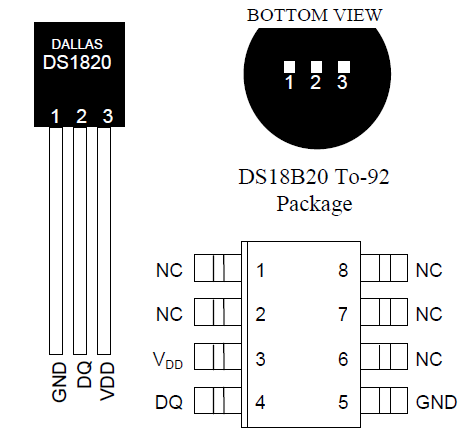
\includegraphics[width=0.6\linewidth]{Imagens/PinTemp.png}
    \smallcaption{Fonte: \textcite{DS18B20}.}
    \label{fig:PinTemp}
\end{figure}

Outras vantagens deste sensor incluem sua capacidade de funcionamento sem outros componentes, o que elimina a necessidade de uma placa de interpretação, por exemplo, além de um intervalo de medição de temperatura satisfatório ao projeto, variando entre ${-55}^{\circ}C$ a ${+125}^{\circ}C$, com uma resolução padrão de $0,5^{\circ}C$, configurável até $0,0625^{\circ}C$ a partir de uma alteração do número de \textit{bits} utilizados para leitura. 

De acordo com seu \textit{datasheet}, \textcite{DS18B20}, de onde foram extraídos os dados supramencionados, este equipamento opera, de maneira simplificada, com base em uma variação de tensão produzida conforme alteração da temperatura, que por sua vez é convertida como um sinal digital e armazenada na memória interna do dispositivo, composta por $16$ \textit{bits} e denominada de \textit{scratchpad}. Este valor é enviado ao controlador, que recebe e armazena os dados coletados. O diagrama de blocos referente ao sensor pode ser visto na Figura \ref{fig:DiagBlocTemp}. 

\begin{figure}[!htb]
\centering
    \caption{Diagrama de blocos para o sensor DS18B20}
    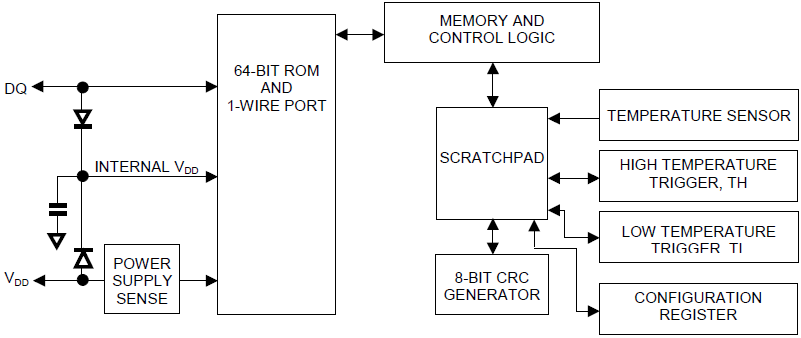
\includegraphics[width=0.8\linewidth]{Imagens/DiagBlocTemp.png}
    \smallcaption{Fonte: \textcite{DS18B20}.}
    \label{fig:DiagBlocTemp}
\end{figure}

Além das vantagens já mencionadas, outro benefício deste equipamento relevante ao trabalho desempenhado diz respeito à sua função de alarme, que funciona a partir dos gatilhos presentes "\textit{HIGH TEMPERATURE TRIGGER, TH}" e "\textit{LOW TEMPERATURE TRIGGER, TL}", vistos também na Figura \ref{fig:DiagBlocTemp}, para altas e baixas temperaturas, respectivamente. Contanto que a função tenha sido especificada no código que roda no controlador, um conjunto de sensores DS18B20 em paralelo pode perceber uma variação acima dos limites definidos pelo usuário e acusar qual sensor recebeu esta informação, indicando, por exemplo, uma discrepância maior de temperatura na região próxima à abertura das portas do carro. Existem diversas bibliotecas para o uso desse sensor, como a \textit{Arduino Temperature Control Library} do \textcite{Arduino-Temperature-Control-Library}.

A respeito do sensor de umidade selecionado, HDC1080, seu \textit{datasheet}, \textcite{HDC1080}, revela que opera em um intervalo de voltagem similar ao de temperatura, de $2,7$ a $5,5$ \textit{Volts}, além de possuir uma precisão satisfatória quanto à obtenção de valores de umidade relativa, variando em apenas 2\%, validando a coleta de dados. Outras vantagens incluem o baixo consumo energético e pequeno tamanho, o que facilita a montagem no espaço à ser utilizado dentro do vagão. A pinagem necessária pode ser vista na Figura \ref{fig:PinHum}, onde \textit{SDA} representa a linha serial de dados, que deve ser conectada ao controlador, transmitindo em velocidade padrão de $11$ \textit{bits} por segundo, \textit{SCL} representa o relógio serial, que mantém o conjunto controlador/sensor em sincronia, e \textit{GND}, \textit{VDD}, e "NC" cumprem as mesmas funções previamente citadas.

\begin{figure}[!htb]
\centering
    \caption{Diagrama da pinagem do sensor HDC1080}
    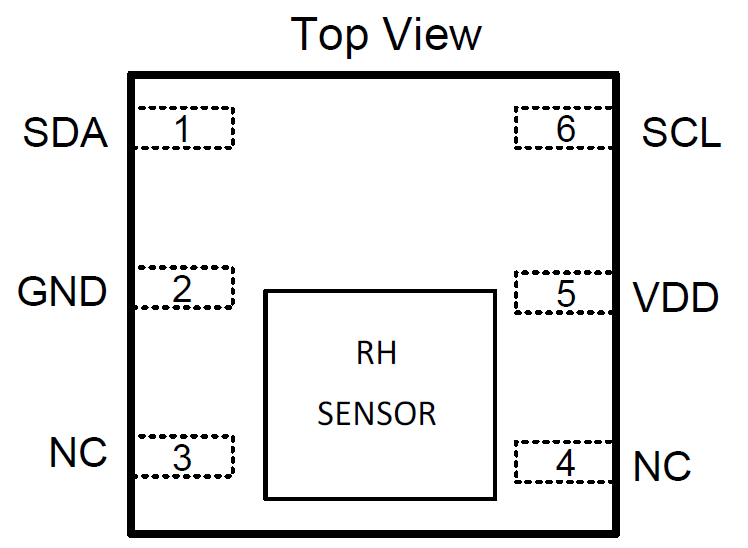
\includegraphics[width=0.4\linewidth]{Imagens/PinHum.png}
    \smallcaption{Fonte: \textcite{HDC1080}.}
    \label{fig:PinHum}
\end{figure}

Existem outros motivos que levaram a escolha deste sensor, dentre eles a ótima reputação de seu fabricante, \textit{Texas Instruments}, que sugere dentro do próprio \textit{datasheet} a aplicação em sistemas de \textit{HVAC}, condizendo com o caso estudado pelo grupo, mas também a presença de um sensor secundário de temperatura. Este sensor será de grande auxílio as análises, pois apresentará um carácter de validação ao trabalhar em conjunto com os sensores de temperatura já utilizados, tanto do metrô, quanto o escolhido pelo grupo. A partir de um conjunto de sensores com a mesma função, é possível confirmar que os dados colhidos condizem com a realidade, descobrir padrões, ou ainda encontrar um aparelho defeituoso, por exemplo. 

Assim, é de interesse do grupo utilizar este sensor suplementar, que opera de modo muito similar ao sensor de temperatura previamente mencionado, em conjunto com a leitura da umidade, que ocorre com a reação entre a camada de poliamida do sensor e a umidade do ar, que é traduzida para um valor de resistência, e pode por sua vez ser interpretada como um sinal digital no controlador. Um diagrama de blocos que representa a operação pode ser visto na Figura \ref{fig:DiagBlocHum}, onde "MCU" representa o controlador.

\begin{figure}[!htb]
\centering
    \caption{Diagrama de blocos para o sensor HDC1080}
    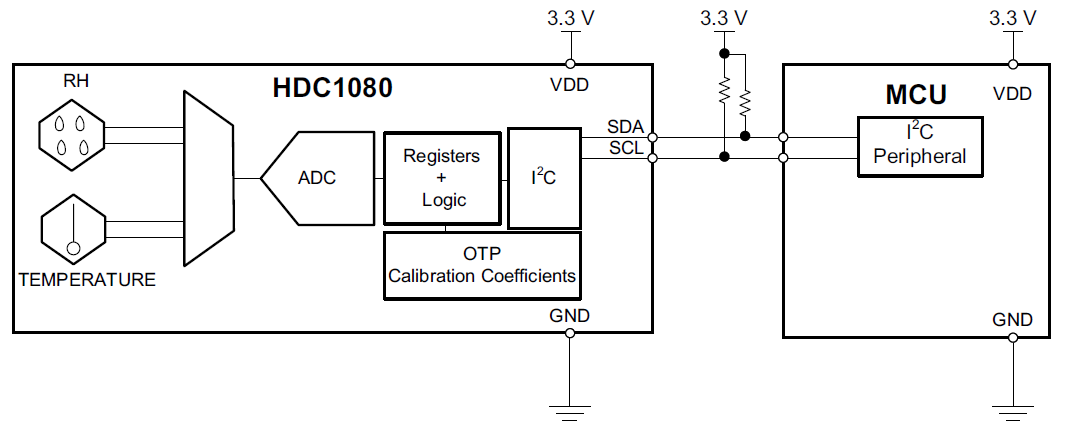
\includegraphics[width=0.75\linewidth]{Imagens/DiagBlocHum.png}
    \smallcaption{Fonte: \textcite{HDC1080}.}
    \label{fig:DiagBlocHum}
\end{figure}

Outras vantagens deste sensor incluem a funcionalidade \textit{HEAT}, que aquece o sensor de modo à reduzir a condensação que pode se acumular no próprio, derivada especialmente de uma operação próxima à um sistema de ar condicionado, além de seu próprio modo de funcionamento, que se divide em um modo de operação, onde o sensor aquisita e envia seus dados, e um modo dormente, onde permanece aguardando uma nova coleta e consumindo quantidades negligenciáveis de energia. A biblioteca existente para esse sensor é a \textit{ClosedCube} HDC1080 \textit{Arduino} do \textcite{ClosedCubeHDC1080}.

Sobre o sensor de ${CO}_{2}$, o modelo escolhido foi o SCD30, produzido pela \textit{SENSIRION}. De acordo com seu \textit{datasheet}, \textcite{SCD30}, sua voltagem de operação varia de $3,3$ a $5,5$ \textit{Volts}, sendo capaz de realizar medições dentro do intervalo de $400$ a $10000$ \textit{partes por milhão} para uma variação de apenas $30$ $ppm$. Este modelo já vem calibrado de fábrica, entretanto o fabricante revela que para resultados mais precisos, é ideal mantê-lo energizado por aproximadamente uma semana em ambiente externo, que geralmente apresenta baixo índice de dióxido de carbono. O consumo de corrente médio é de $19$ $mA$, chegando à um máximo de $75$ $mA$ durante as medições, além de operar em temperaturas de $0$ a $50$ $^{\circ}C$, o que é satisfatório para o projeto. 

Um diagrama indicando a pinagem do sensor pode ser visto na Figura \ref{fig:PinCO2}, onde \textit{VDD} e \textit{GND} cumprem as mesmas funções já mencionadas, \textit{TX/SCL} faz a transferência de dados do sensor para o controlador, além do relógio serial, \textit{RX/SDA} recebe informações vindas do controlador, como um pedido de início de medição, por exemplo, \textit{RDY} indica que os dados estão prontos para coleta, \textit{PWM} envia um valor de voltagem variável que indica a concentração de ${CO}_{2}$ e \textit{SEL} seleciona as diferentes interfaces do sensor.

\begin{figure}[!htb]
\centering
    \caption{Diagrama da pinagem do sensor SCD30}
    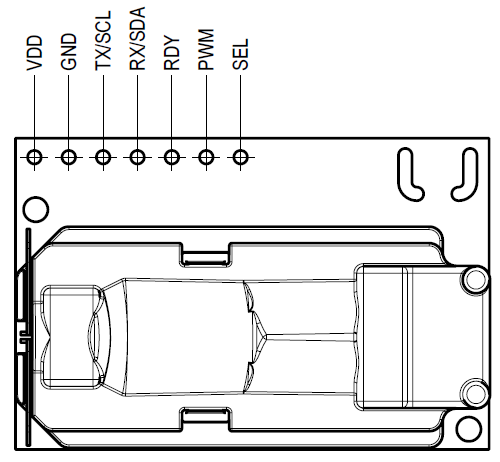
\includegraphics[width=0.5\linewidth]{Imagens/PinCO2.png}
    \smallcaption{Fonte: \textcite{SCD30}.}
    \label{fig:PinCO2}
\end{figure}

Este dispositivo utiliza a tecnologia \textit{NDIR} , ou \textit{Nondispersive infrared}, para realizar a leitura dos níveis de ${CO}_{2}$ no ambiente. De maneira simplificada, o sensor utiliza um pequeno diodo emissor de luz infravermelha instalado dentro de um tubo que se comunica com o ambiente via uma entrada e saída.  Neste invólucro, há também um sensor óptico baseado nas características de uma molécula de ${CO}_{2}$,  de modo que quando o ar dentro deste tubo é bombardeado com a luz mencionada, há uma absorção dos raios por parte das moléculas do gás analisado, fazendo com que o sensor óptico, ao realizar a leitura, obtenha uma concentração menor do que a prévia, para um caso de aumento da substância estudada, por exemplo \cite{NDIR}. Esta diferença é, então, contabilizada pelo sensor que, por sua vez, envia os dados para o controlador, e assim a medição é concluída.

É válido citar que, de modo similar ao sensor de umidade escolhido, este sensor de ${CO}_{2}$ também possui equipamentos redundantes ao projeto, como um sensor de temperatura e um de umidade relativa, ambos com características satisfatórias ao necessário para a análise. Como já foi citado, estes sensores auxiliares validam as coletas realizadas, garantindo uma maior credibilidade ao estudo. Além disso, a presença deste sensor dispensa a necessidade de outro para aquisição de ${O}_{2}$, visto que este parâmetro pode ser estimado a partir dos resultados obtidos. A biblioteca existente para esse sensor é a \textit{Adafruit} SCD30 da \textcite{Adafruit_SCD30}. 

Por fim, a respeito do último sensor selecionado, pode-se citar o BMP280, produzido pela \textit{BOSCH}, como o sensor de pressão barométrica escolhido para o projeto. Este sensor realiza a medição da pressão atmosférica absoluta em um intervalo de $300$ a $1100$ $hPa$, equivalente a aproximadamente $+9000$ (acima) e $-500$ (abaixo) metros do nível do mar, com uma precisão de $\pm$ $0,12$ $hPa$, equivalente a $\pm$ $1$ $metro$. O sensor realiza estas medições para uma voltagem de $1,7$ a $3,3$ \textit{Volts}, consumindo uma corrente muito baixa, de $2,7$ $\mu$$A$, além de operar dentro de um intervalo de temperatura de $-40$ a $85$ $^{\circ}C$, condições propícias ao projeto. Entre outras vantagens, há seu pequeno tamanho, visto que foi desenvolvido para aplicações \textit{mobile}, ou seja, para dispositivos móveis, facilitando o posicionamento em sua respectiva placa.

A escolha deste sensor foi facilitada, ao considerar além das especificações já mencionadas, a reputação de seu fabricante, que possui anos de experiência nesta e em outras áreas de aplicação. Assim, descrevendo as conexões realizadas com o controlador, tem se a Figura \ref{fig:PinPress}, onde \textit{VCC} e \textit{GND} realizam as mesmas funções já citadas, mas para uma conexão de $3,3$ \textit{Volts}, \textit{SCL} representa a entrada do relógio serial, \textit{SDA} representa a entrada de dados vindos do controlador, \textit{CSB} representa o seletor de interfaces, já que o sensor pode operar com diferentes controladores (neste caso, deve ser conectado à uma tensão secundária), e \textit{SDO} realiza o envio dos dados coletados pelo sensor para o controlador. É válido citar que, enquanto estas informações foram extraídas do \textit{datasheet}, \textcite{BMP280}, este não é o caso da Figura \ref{fig:PinPress}, pois o documento mencionado apresenta diretamente as conexões feitas ao microchip, isto é, diretamente ao sensor, que necessita de uma placa secundária para interface com o controlador selecionado devido ao seu pequeno tamanho.

\begin{figure}[!htb]
\centering
    \caption{Definição de pinos do BMP280}
    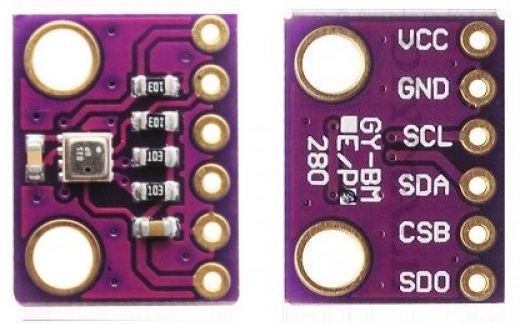
\includegraphics[width=0.25\linewidth]{Imagens/PinPress.png}
    \smallcaption{Fonte: \textcite{imgBMP280}.}
    \label{fig:PinPress}
\end{figure}

A respeito de seu princípio de funcionamento, denominado de piezo resistivo, o mesmo ocorre com a deformação de um diafragma interno por efeito de uma pressão aplicada, geralmente construído de silicone e calibrado com base na pressão a ser medida, neste caso a atmosférica, que é notada por um \textit{strain gauge}, ou seja, um extensômetro, o que causa uma alteração na resistência percebida na ponte de \textit{Wheatstone} presente dentro do componente. De maneira análoga, conforme a resistência é alterada, a voltagem que passa pelo sensor também sofre uma alteração, o que pode ser enviado para o controlador e interpretado como a pressão atmosférica do ambiente presente \cite{piezo}, sendo um exemplo disto visto na Figura \ref{fig:piezoresist}.

\begin{figure}[!htb]
\centering
    \caption{Princípio de funcionamento de um sensor piezo resistivo}
    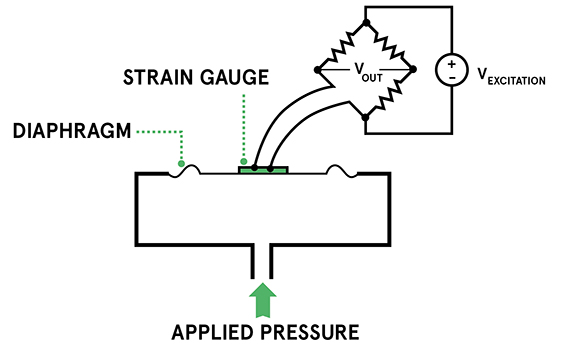
\includegraphics[width=0.4\linewidth]{Imagens/piezoresist.jpg}
    \smallcaption{Fonte: \textcite{imgpiezo}.}
    \label{fig:piezoresist}
\end{figure}

A partir da medição de pressão barométrica, este sensor permite, portanto, o cálculo da altitude em que se encontra, informação relevante para a obtenção da situação climática, por exemplo. Outro ponto extremamente importante, visto até como o principal motivo para a escolha de um sensor de pressão, é a necessidade deste valor para que a umidade relativa, obtida com os outros sensores, possa ser convertida corretamente para umidade absoluta, fator mais explorado nas seções \ref{balenergia} e \ref{VGD}. Além disso, como outra vantagem, este equipamento também possui um sensor de temperatura redundante ao projeto, que será usado com o mesmo propósito de validação de dados. A biblioteca existente para esse sensor é a \textit{Adafruit} BMP280 da \textcite{Adafruit_BMP280}. 

\subsection{Protoboard} \label {Proto}

A partir das escolhas dos sensores na seção \ref{sensor}, conseguiu-se fazer a seleção do microcontrolador. Segundo \textcite{kerschbaumer2013microcontroladores}, os microcontroladores são circuitos integrados que possuem em seu interior todos os componentes necessários para seu funcionamento dependendo unicamente da fonte de alimentação externa. Logo, eles agem como o cérebro de toda a parte eletrônica responsável pelo fluxo de dados e a computação dos mesmos.

A placa de prototipagem escolhida foi o \textit{Arduino Nano}, Figura \ref{fig:pinagem arduino}, integrada pelo microcontrolador \textit{ATmega328} \cite{UNO}. A principal vantagem da escolha da plataforma \textit{Arduino}, além do seu custo relativamente acessível, é a facilidade para desenvolver software com ela. A linguagem para desenvolver códigos é uma versão simplificada de \textit{C} e \textit{C++}, e para contribuir ainda mais existem na casa de milhões de bibliotecas online, que são programas que foram criados por outros usuários de modo a facilitar a interface com diferentes componentes, como os sensores que serão utilizados neste projeto, podendo ser usadas gratuitamente dado a natureza do ecossistema \textit{Arduino}, facilitando assim boa parte do desenvolvimento do algorítimo base. Os sensores escolhidos já possuem bibliotecas pré-estabelecidas que serão utilizadas pelo grupo.

\begin{figure}[!htb]
\centering
    \caption{Pinagem do Arduino Nano}
    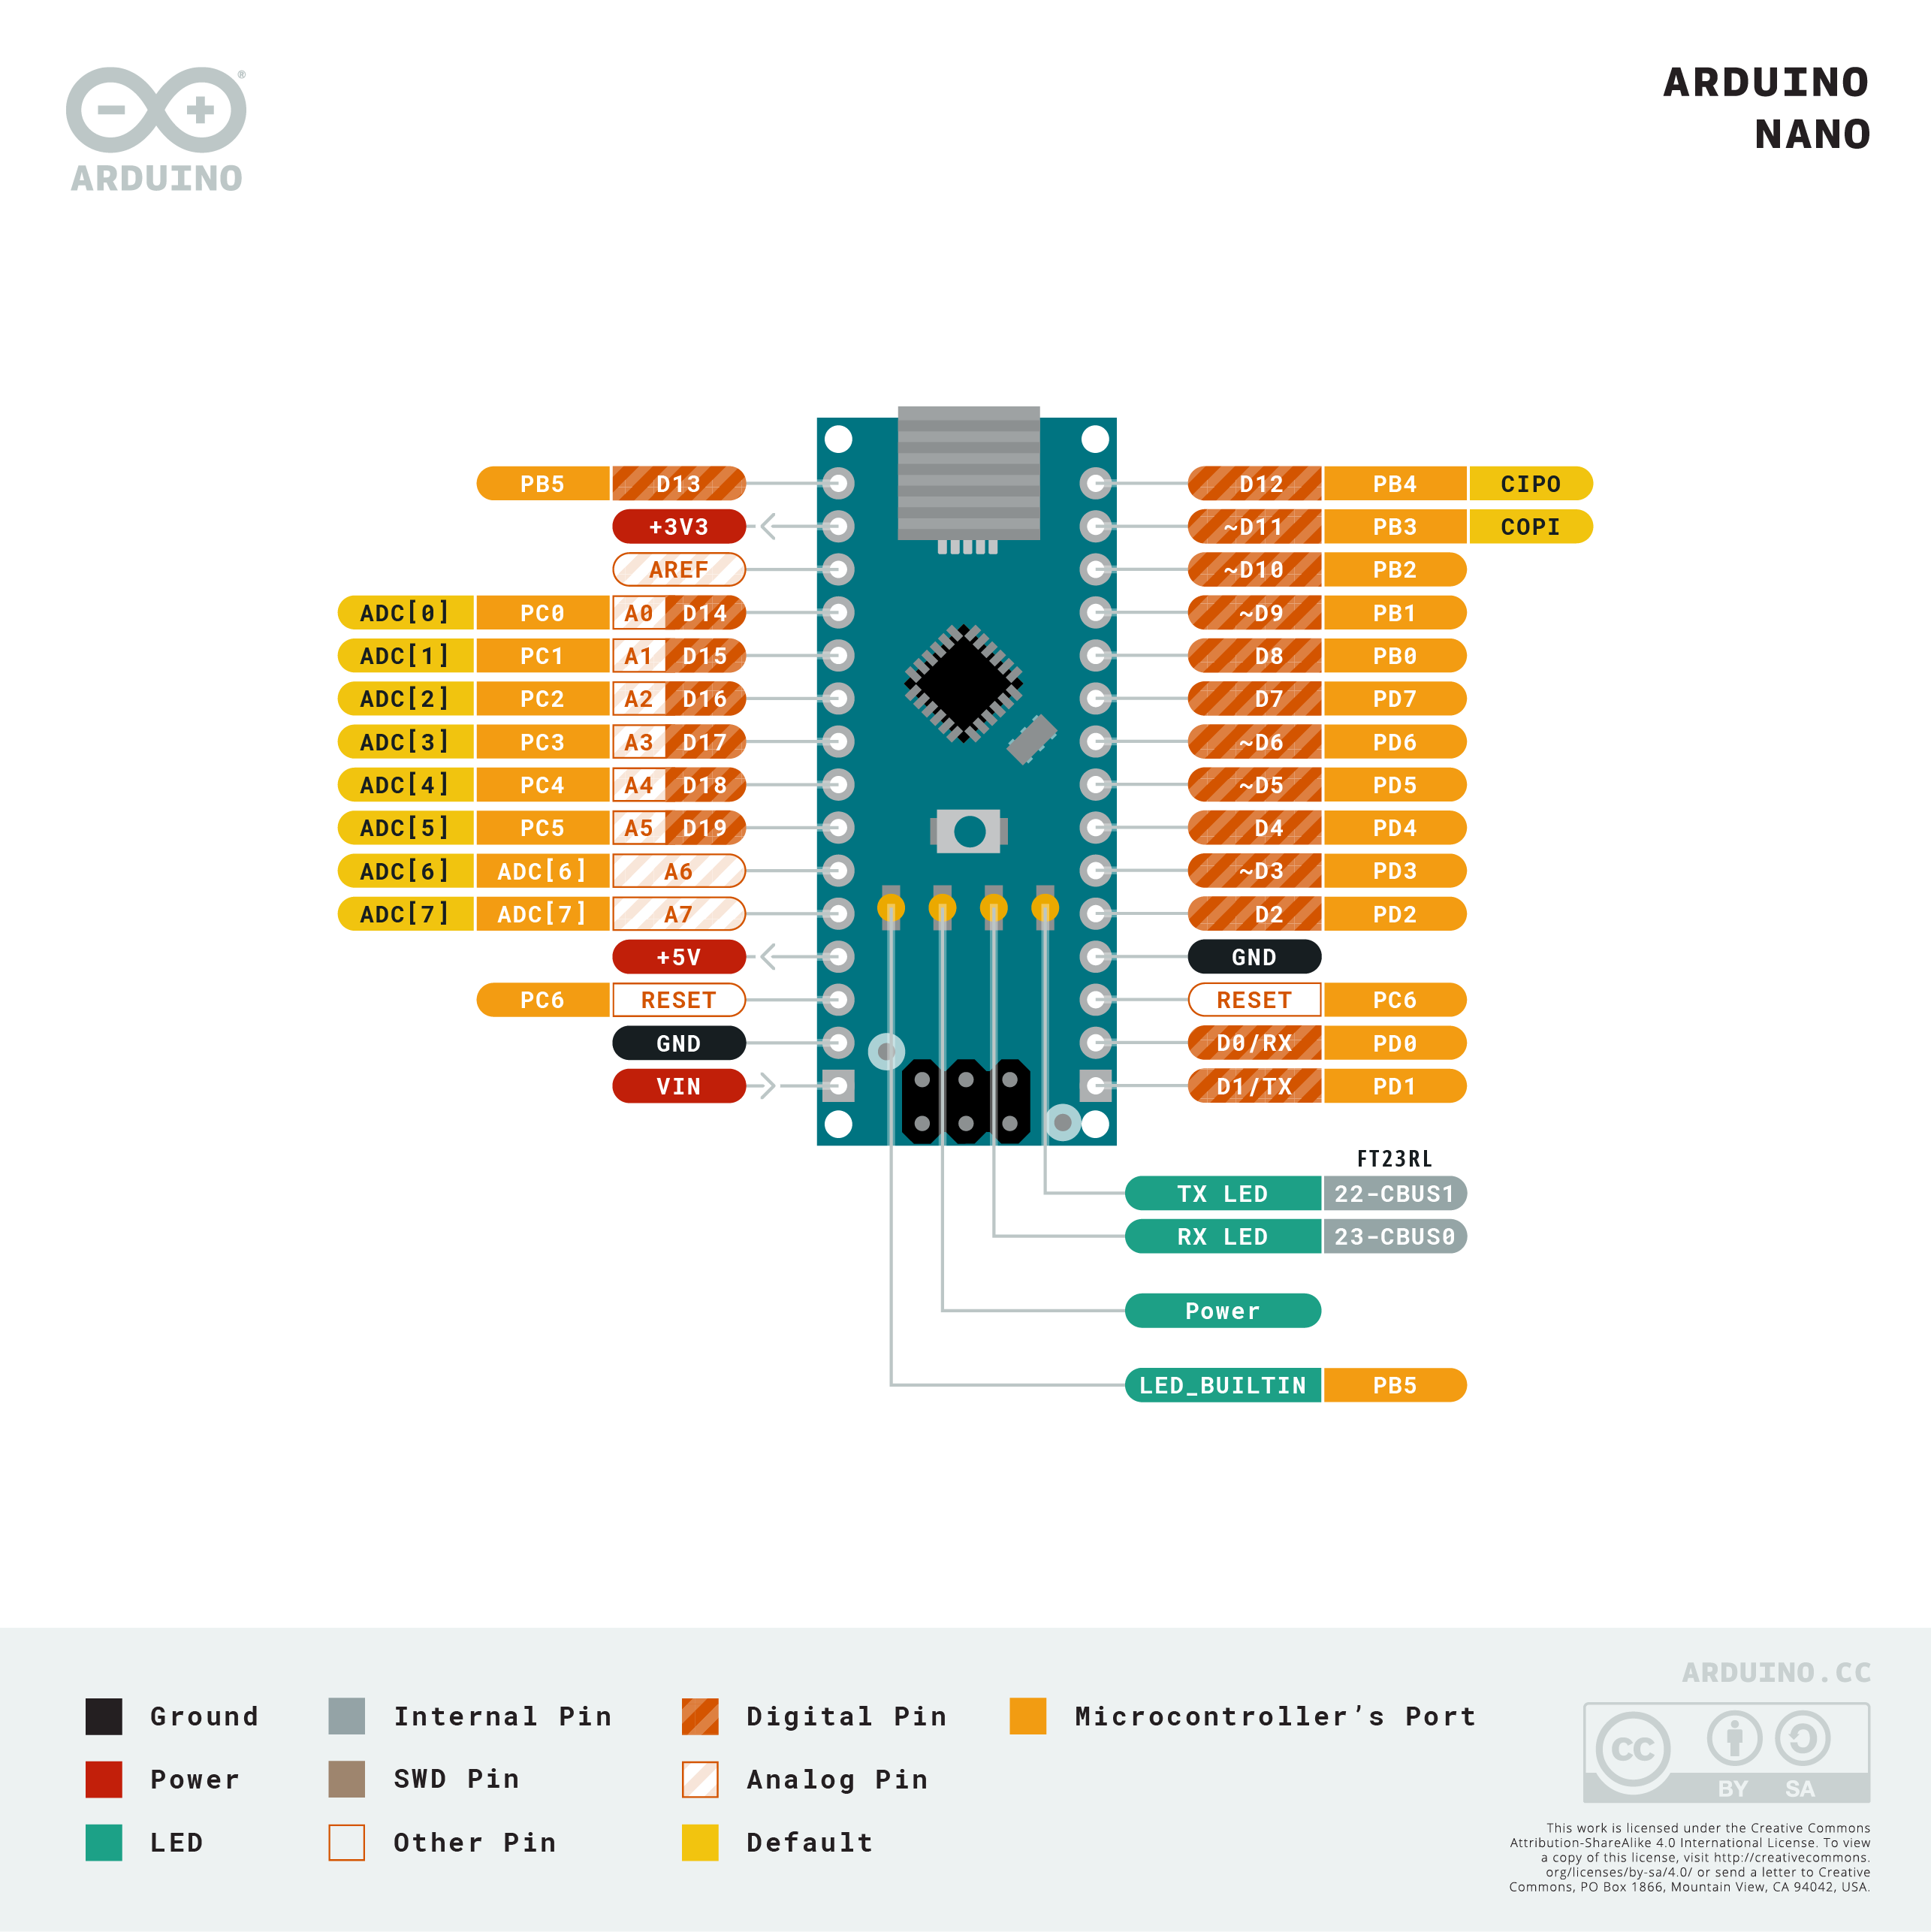
\includegraphics[width=0.85\linewidth]{Imagens/Pinagem_Arduino_Nano.png}
    \smallcaption{Fonte: \textcite{UNO}}
    \label{fig:pinagem arduino}
\end{figure}

Para armazenamento de dados será utilizado o \textit{Módulo Micro SD Card}, Figura \ref{fig:FotomicroSD}, que é um adaptador que transfere os dados gerados pelos sensores e interpretados pelo \textit{Arduino} para um cartão \textit{Micro SD} externo removível, pois o \textit{Arduino Nano} possui $32$ $kB$ \textit{flash} de memória \cite{UNO}, com o papel de armazenar o programa feito para ler os sensores e os dados gerados pelos mesmos. Com a utilização do \textit{Módulo Micro SD Card} é possível transferir todos os dados gerados em um cartão \textit{Micro SD} que pode ser de $2$ $GB$ até $2$ $TB$ de memória, resolvendo o problema de armazenamento e conseguindo registrar o máximo de dados que os sensores puderem fornecer. A vantagem de usar um cartão \textit{Micro SD} para o armazenamento é que já existem bibliotecas acessíveis para seu uso, como a desenvolvida pelo próprio \textit{Arduino}, denominada apenas de \textit{SD}, e encontrada pré-instalada no \textit{Arduino IDE}, como apresentado por \textcite{ArdMicroSD}. Para a análise de seu funcionamento foi adicionado um \textit{LED} ao Arduino que varia conforme a leitura ocorre. Caso o cartão SD não seja reconhecido, o \textit{LED} permanece aceso, até que apaga após resolução do problema. Entretanto, no caso de ser reconhecido mas o arquivo não está sendo gravado corretamente, o mesmo pisca, e, novamente, apaga após o funcionamento normal resumir.

\begin{figure}[!htb]
\centering
    \caption{\textit{Módulo Micro SD Card}}
    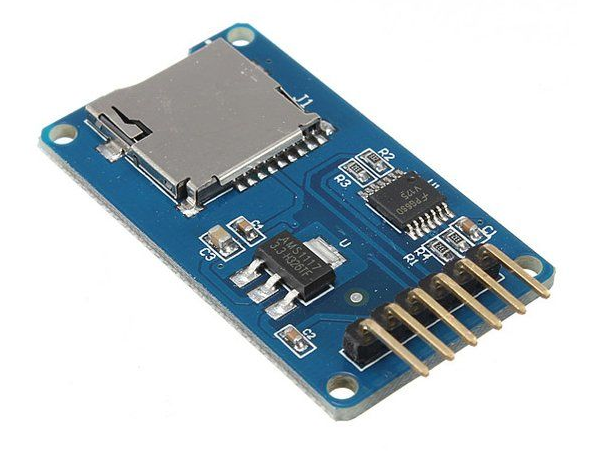
\includegraphics[width=0.3\linewidth]{Imagens/microsd.png}
    \smallcaption{Fonte: \textcite{prototype}}
    \label{fig:FotomicroSD}
\end{figure}

Com a seleção do microcontrolador e do sistema de armazenamento, é possível seguir para o esquemático e montagem das \textit{protoboards}, que são as placas de teste que permitem a montagem de circuitos eletrônicos temporários, com a função de testar o funcionamento dos componentes e o código desenvolvido.

Usando como base todos os \textit{datasheets} dos componentes e o uso do software \textit{KiCAD}, foi possível fazer os primeiros esquemáticos, Figuras \ref{fig:footprintprotoboardint} e \ref{fig:footprintpressao}, que apresentam todos os componentes e conectores escolhidos, alimentados por uma fonte regulada de $5$ $V$, que é a tensão em que o \textit{Arduino Nano} e uma parte dos componentes operam. Assim, tanto para o Kit Conforto quanto o Kit Pressão, a ideia do grupo consiste em utilizar bancos de baterias portáteis, popularmente conhecidos como \textit{Power Banks}, que possibilitam alimentar as placas corretamente com 5 \textit{Volts}.

\begin{figure}[!htb]
\centering
    \caption{\textit{Footprint} para montar a \textit{protoboard} - Kit Conforto}
    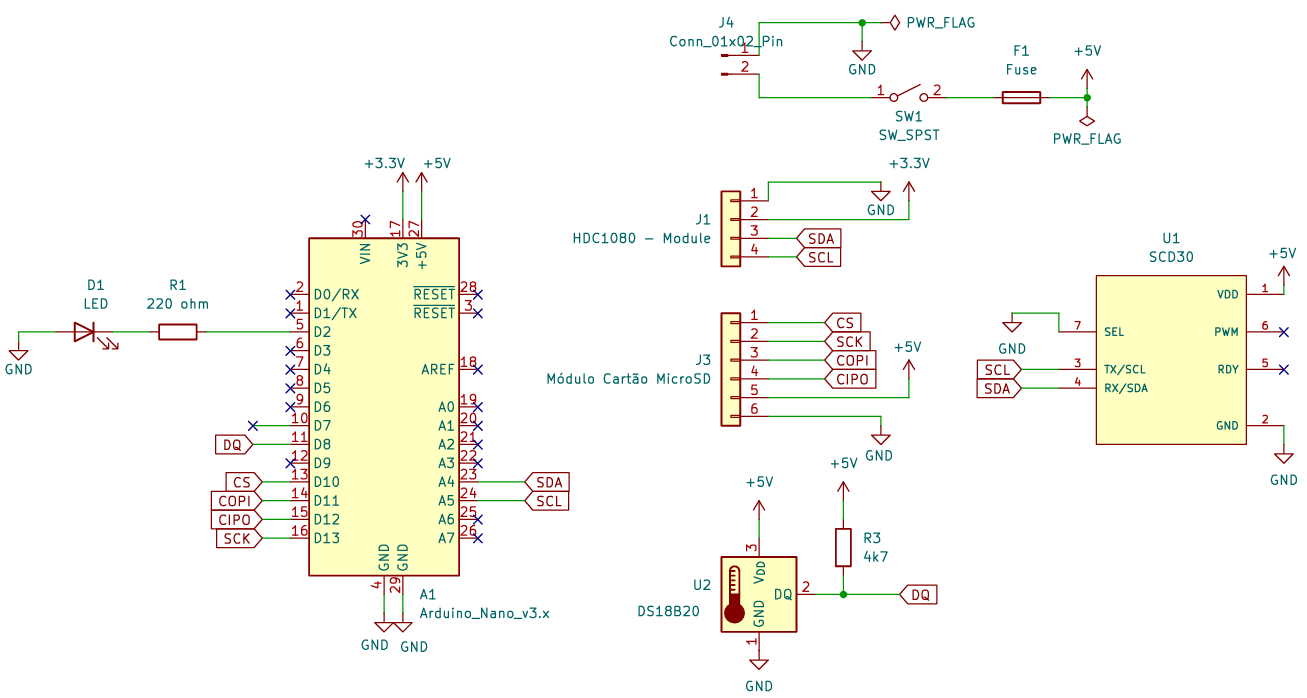
\includegraphics[width=1\linewidth]{Imagens/footprintprotoboardint.png}
    \smallcaption{Fonte: Autor}
    \label{fig:footprintprotoboardint}
\end{figure}

\begin{figure}[!htb] 
\centering
    \caption{\textit{Footprint} para montar a \textit{protoboard} - Kit Pressão}
    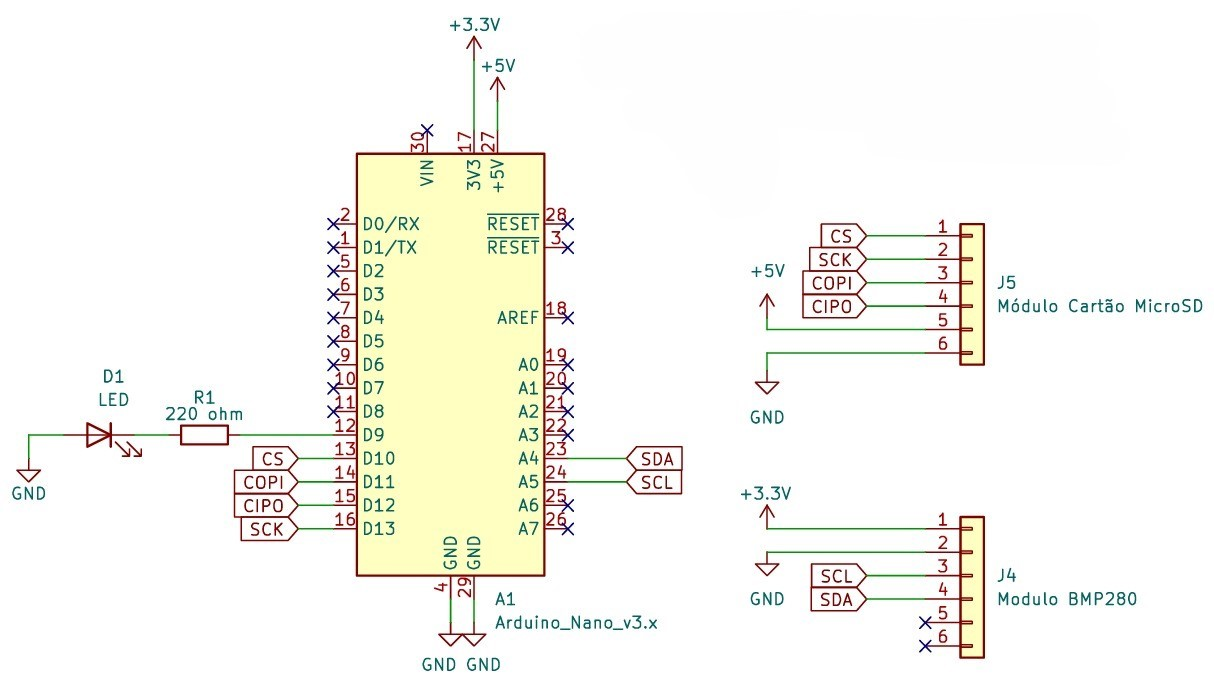
\includegraphics[width=1\linewidth]{Imagens/footprintpressao.jpg} 
    \smallcaption{Fonte: Autor}
    \label{fig:footprintpressao}
\end{figure}

De modo a comprovar e validar os \textit{footprints} apresentadas nas Figuras \ref{fig:footprintprotoboardint} e \ref{fig:footprintpressao}, pode se apresentar as \textit{protoboards} nas Figuras \ref{fig:protoconforto} e \ref{fig:protopressao}, que representam a montagem do kit em um estágio anterior às \textit{PCBs}, pois possuem o exato comportamento esperado do produto final, mas em um formato facilmente alterado, caso ocorram problemas. Assim, é possível testar tanto o código quanto os componentes adquiridos, garantindo que tudo funcione para os dias de coleta de dados.

\begin{figure}[!htb]
\centering
    \caption{\textit{Protoboard} montada - Kit Conforto}
    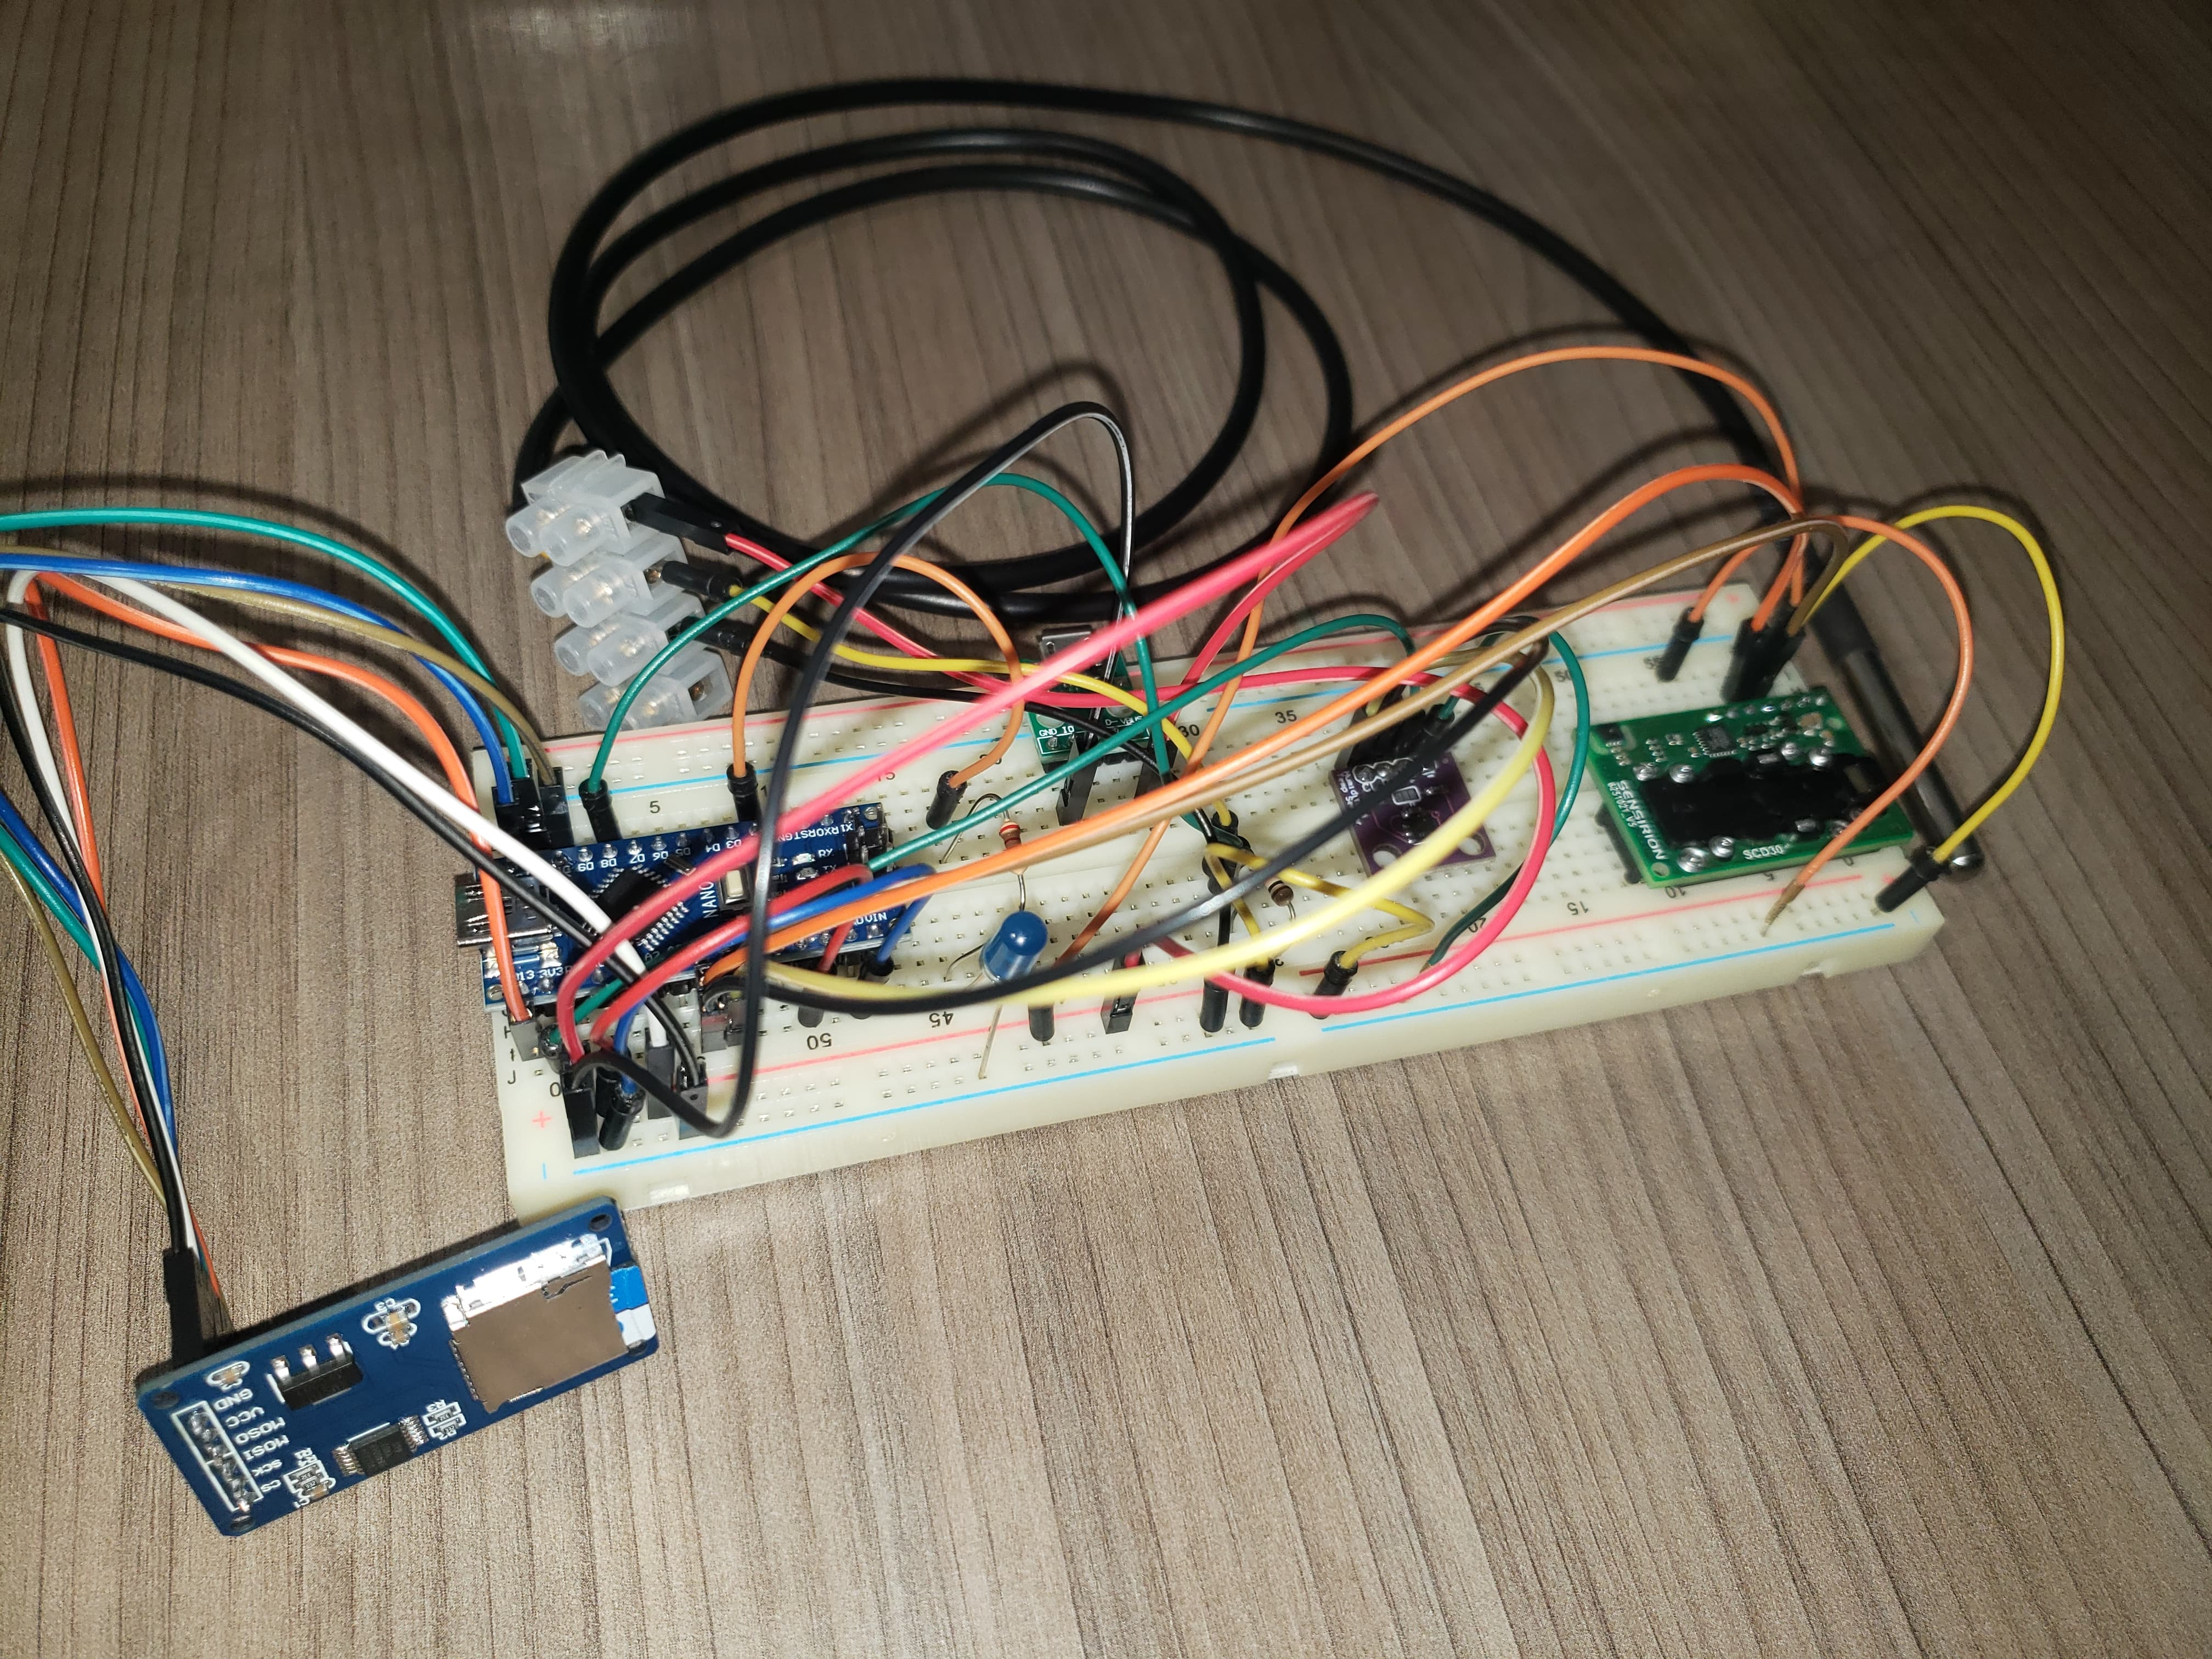
\includegraphics[width=0.65\linewidth]{Imagens/protoboardmovel.jpeg}
    \smallcaption{Fonte: Autor}
    \label{fig:protoconforto}
\end{figure}

\begin{figure}[!htb]
\centering
    \caption{\textit{Protoboard} montada - Kit Pressão}
    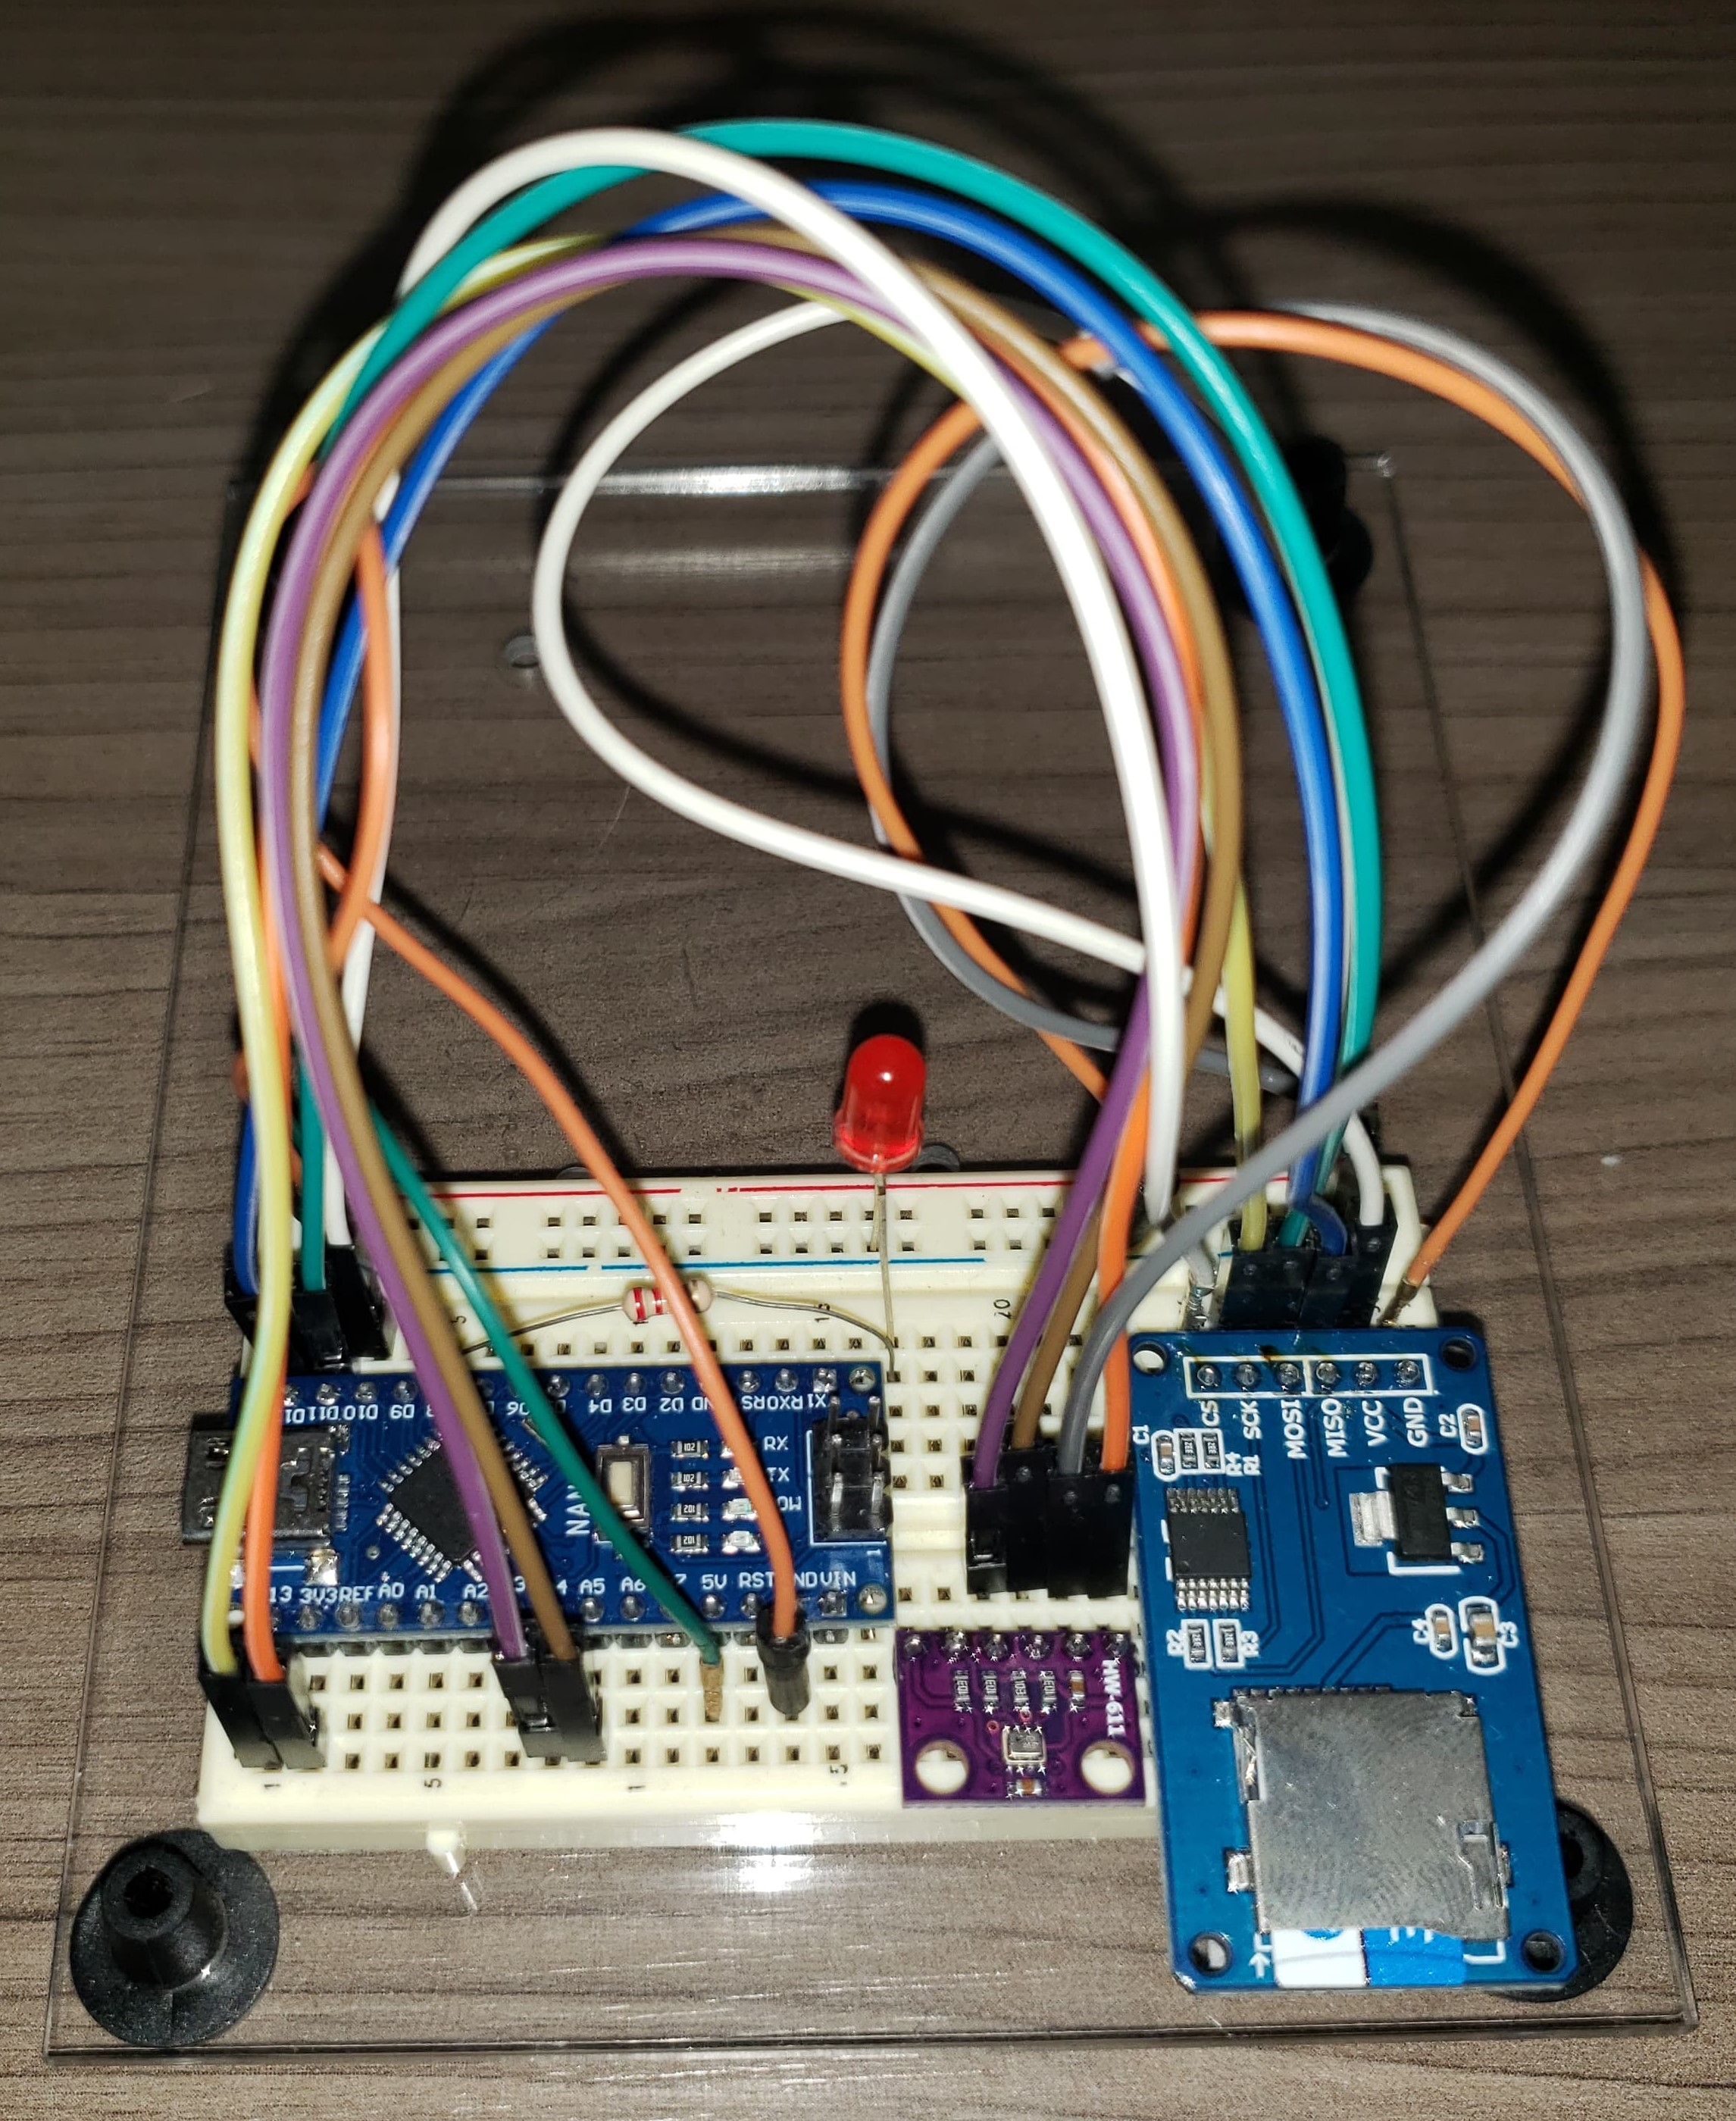
\includegraphics[width=0.45\linewidth]{Imagens/protoboardpressao.jpeg}
    \smallcaption{Fonte: Autor}
    \label{fig:protopressao}
\end{figure}

Uma vez montadas as \textit{protoboards}, já com o código que as acompanha bem definido, houve uma fase de testes que durou pouco mais de uma semana. Este tempo foi gasto de modo a, como dito anteriormente nesta seção, validar o funcionamento de todo o conjunto, mas também para realizar a calibração correta dos sensores, como é especificado pelos fabricantes nos \textit{datasheets} de cada sensor utilizado. O sensor de ${CO}_{2}$, por exemplo, requer um período de sete dias energizado em um local aberto, para que possa estabelecer um padrão e entender o que é um ambiente com baixos níveis de gás carbônico, o que em troca resulta numa instrumentação mais precisa. Além disso, o grupo também buscou entender melhor a questão da alimentação das placas, realizando testes também da utilização dos \textit{Power Banks}, onde o conjunto permaneceu ligado durante tempo suficiente para validar seu funcionamento, sendo esta questão melhor detalhada na seção \ref{PCB} a seguir.

\newpage

\subsection{\textit{Printed Circuit Board (PCB)}} \label{PCB}

A \textit{Printed Circuit Board (PCB)} é o modelo final após a validação com a \textit{protoboard}, onde os componentes geralmente estão soldados à placa, o que garante não só uma estética melhor ao projeto, mas, fator de maior importância, um funcionamento com menor propensão à erros, pois os componentes estão corretamente fixados à placa. Entretanto, deve se considerar que este estágio é final, dificultado alterações no sistema, especialmente em campo, pois neste momento não é comum possuir as ferramentas corretas para isso. Pensando nisso, o grupo optou pela utilização de barras de pinos do tipo macho e fêmea, expostas nas Figuras \ref{fig:barramacho} e \ref{fig:barrafemea}, respectivamente, onde as barras de tipo macho foram soldadas aos componentes, e as de tipo fêmea, às \textit{PCBs}.

\begin{figure}[!htb]
    \centering
    \begin{minipage}{0.45\textwidth}
        \caption{Barra de pinos de tipo macho}
        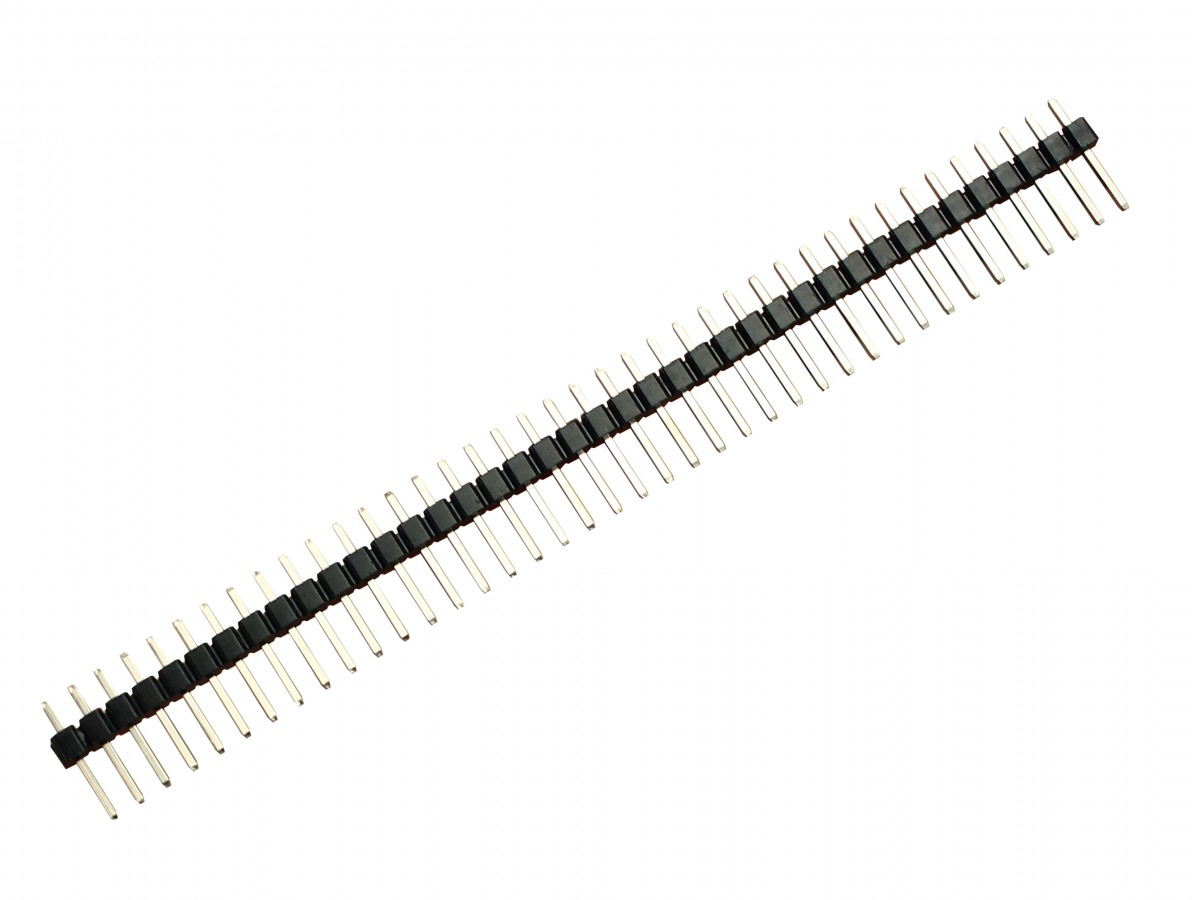
\includegraphics[width=\linewidth, height=6cm]{Imagens/barramacho.jpg}
        \smallcaption{Fonte: \textcite{barrapinomacho}}
        \label{fig:barramacho}
    \end{minipage}\hfill
    \begin{minipage}{0.45\textwidth}
        \caption{Barra de pinos de tipo fêmea}
        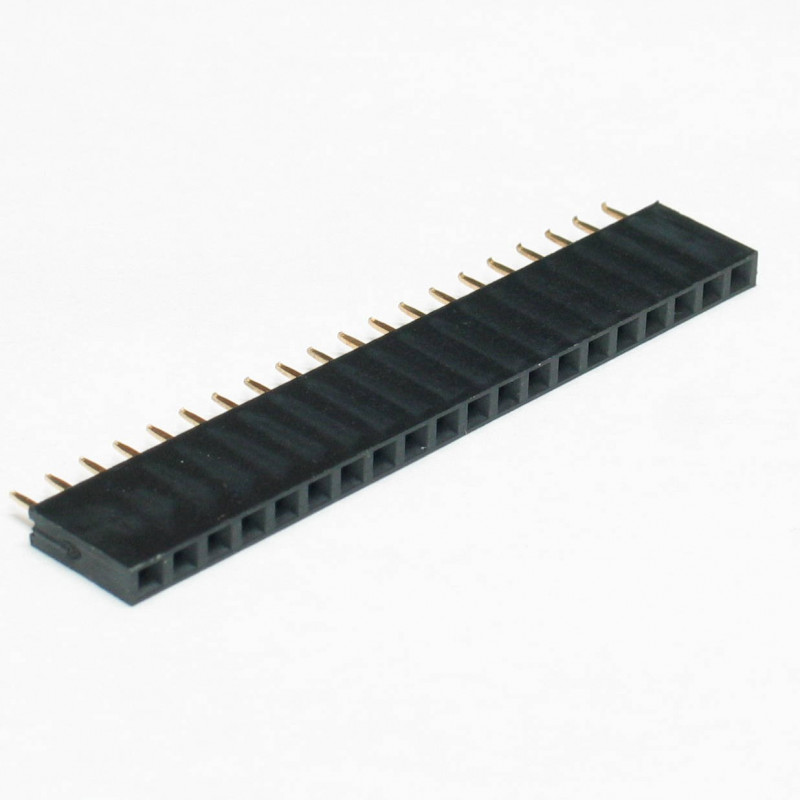
\includegraphics[width=\linewidth, height=6cm]{Imagens/barrafemea.jpg}
        \smallcaption{Fonte: \textcite{barrapinofemea}}
        \label{fig:barrafemea}
    \end{minipage}
\end{figure}

Sabendo que as \textit{PCBs} precisam de uma fonte correta de alimentação pois não utilizarão a energia diretamente da bateria do carro, será utilizado para o Kit Conforto um módulo de adaptação \textit{Micro USB}, Figura \ref{fig:micro_usb}, previsto também na \textit{footprint} do mesmo e funcionando basicamente como uma entrada de energia comum, assim como a vista em alguns modelos de celular, podendo receber carga elétrica de fontes externas reguladas como as baterias externas portáteis citadas na seção \ref{Proto}. Este módulo \textit{Micro USB} foi selecionado somente para o Kit Conforto pois o mesmo apresenta três sensores diferentes, além do módulo de \textit{cartão SD}, assim é considerado uma boa prática não utilizar a entrada \textit{Mini USB} própria do \textit{Arduino Nano} como a principal fonte de energia de modo a não sobrecarregar o regulador de tensão presente o microcontrolador. Este não é o caso do Kit Pressão, que possui apenas o sensor de pressão barométrica e o módulo de \textit{cartão SD}, sendo assim não há problema em alimentá-lo com a tensão oriunda da conexão na porta \textit{Mini USB} do \textit{Arduino}.

\begin{figure}[!htb]
\centering
    \caption{Módulo Adaptador Micro \textit{USB} Fêmea para \textit{DIP}}
    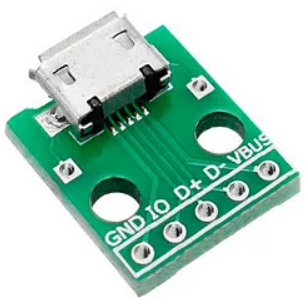
\includegraphics[width=0.25\linewidth]{Imagens/Micro_USB.png}
    \smallcaption{Fonte: \textcite{micro_usb}}
    \label{fig:micro_usb}
\end{figure}

Torna-se válida também uma breve explicação a respeito do método utilizado para obtenção das placas de circuito impresso. Inicialmente, parte-se da geração de uma máscara contendo o desenho do padrão que se deseja imprimir na placa, que originalmente nada mais é do que uma base vazia para a \textit{PCB}, comumente composta por um polímero com um dos lados completamente recoberto por material com alta condutividade elétrica, sendo um dos mais utilizados o cobre. Definido o padrão desejado, a máquina de Controle Numérico de por Computador (CNC) realiza a remoção estratégica de material, deixando trilhas que conectam os componentes, e suas respectivas cavidades, onde serão inseridos e posteriormente soldados \cite{sousaPCB}.  

A partir dos desenhos das \textit {footprints}, foi novamente utilizado o software \textit{KiCAD} de modo a se obter a máscara citada em um formato conveniente para ambos os kits, como é visto nas Figuras \ref{fig:mascaraconfort} e \ref{fig:mascarapressao}, que são posteriormente enviadas à ferramenta presente no Centro Universitário FEI, por fim realizando a usinagem das trilhas requeridas nas placas. Os passos seguintes consistem na separação das placas uma das outras, já que saem no mesmo conjunto, seguida da soldagem das barras de pinos tipo fêmea nas trilhas.

\begin{figure}[!htb]
    \centering
    \begin{minipage}{0.45\textwidth}
        \caption{Máscara para produção do \textit{PCB} do Kit Conforto}
        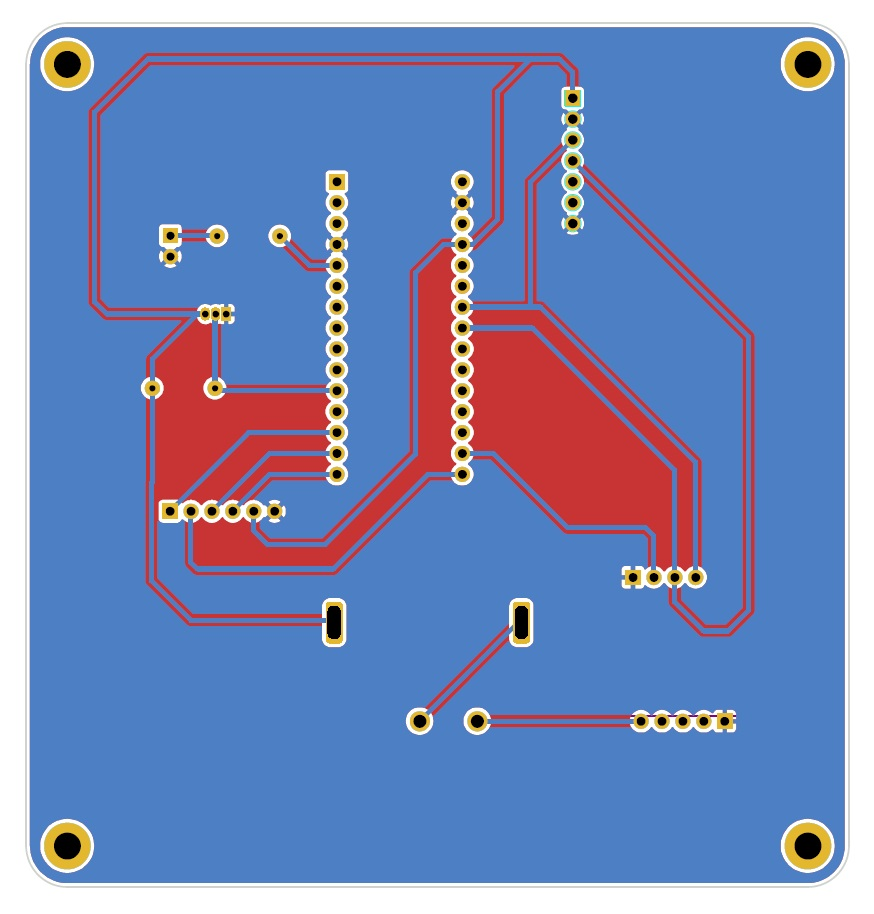
\includegraphics[width=\linewidth, height=7.5cm]{Imagens/mascaraconforto.jpg} 
        \smallcaption{Fonte: Autor}
        \label{fig:mascaraconfort}
    \end{minipage}\hfill
    \begin{minipage}{0.45\textwidth}
        \caption{Máscara para produção do \textit{PCB} do Kit Pressão}
        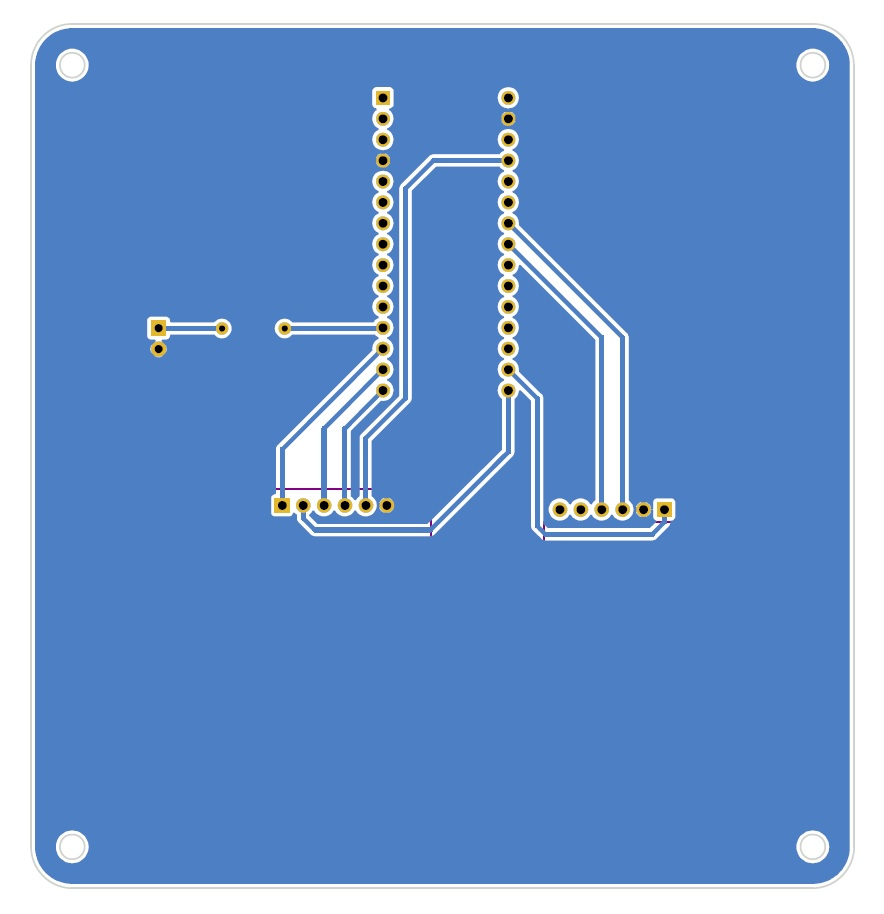
\includegraphics[width=\linewidth, height=7.5cm]{Imagens/mascarapressao.jpg} 
        \smallcaption{Fonte: Autor}
        \label{fig:mascarapressao}
    \end{minipage}
\end{figure}

Visto que o consumo de corrente do conjunto de microcontrolador e componentes escolhidos é relativamente baixo como foi comprovado pelos testes do grupo e exposto nos \textit{datasheets} dos mesmos, foram escolhidos três modelos de bancos de bateria que os integrantes do grupo já possuíam, com capacidade total das baterias de $8800$, $10000$ e $14000$ \textit{mAh}, valores muito acima da necessidade ao se considerar o consumo de fato observado. Deste modo, a partir dos fatos argumentados, é possível apresentar as Figuras \ref{fig:PCB_conforto} e \ref{fig:PCB_Pressao}, onde são expostas uma das três placas montadas para o Kit Conforto conectado a um dos \textit{Power Banks}, com as luzes do \textit{Arduino Nano} acesas indicando seu funcionamento, exercendo sua função de coleta e armazenamento de dados, e o modelo 3D do Kit Pressão, também oriundo do \textit{KiCAD}, onde as barras de pinos fêmea nomeadas de J2 e J3, da esquerda para a direita, representam os locais onde são conectados o módulo de \textit{cartão SD} e o sensor de pressão, respectivamente.

\begin{figure}[!htb]
\centering
    \caption{\textit{PCB} do Kit Conforto}
    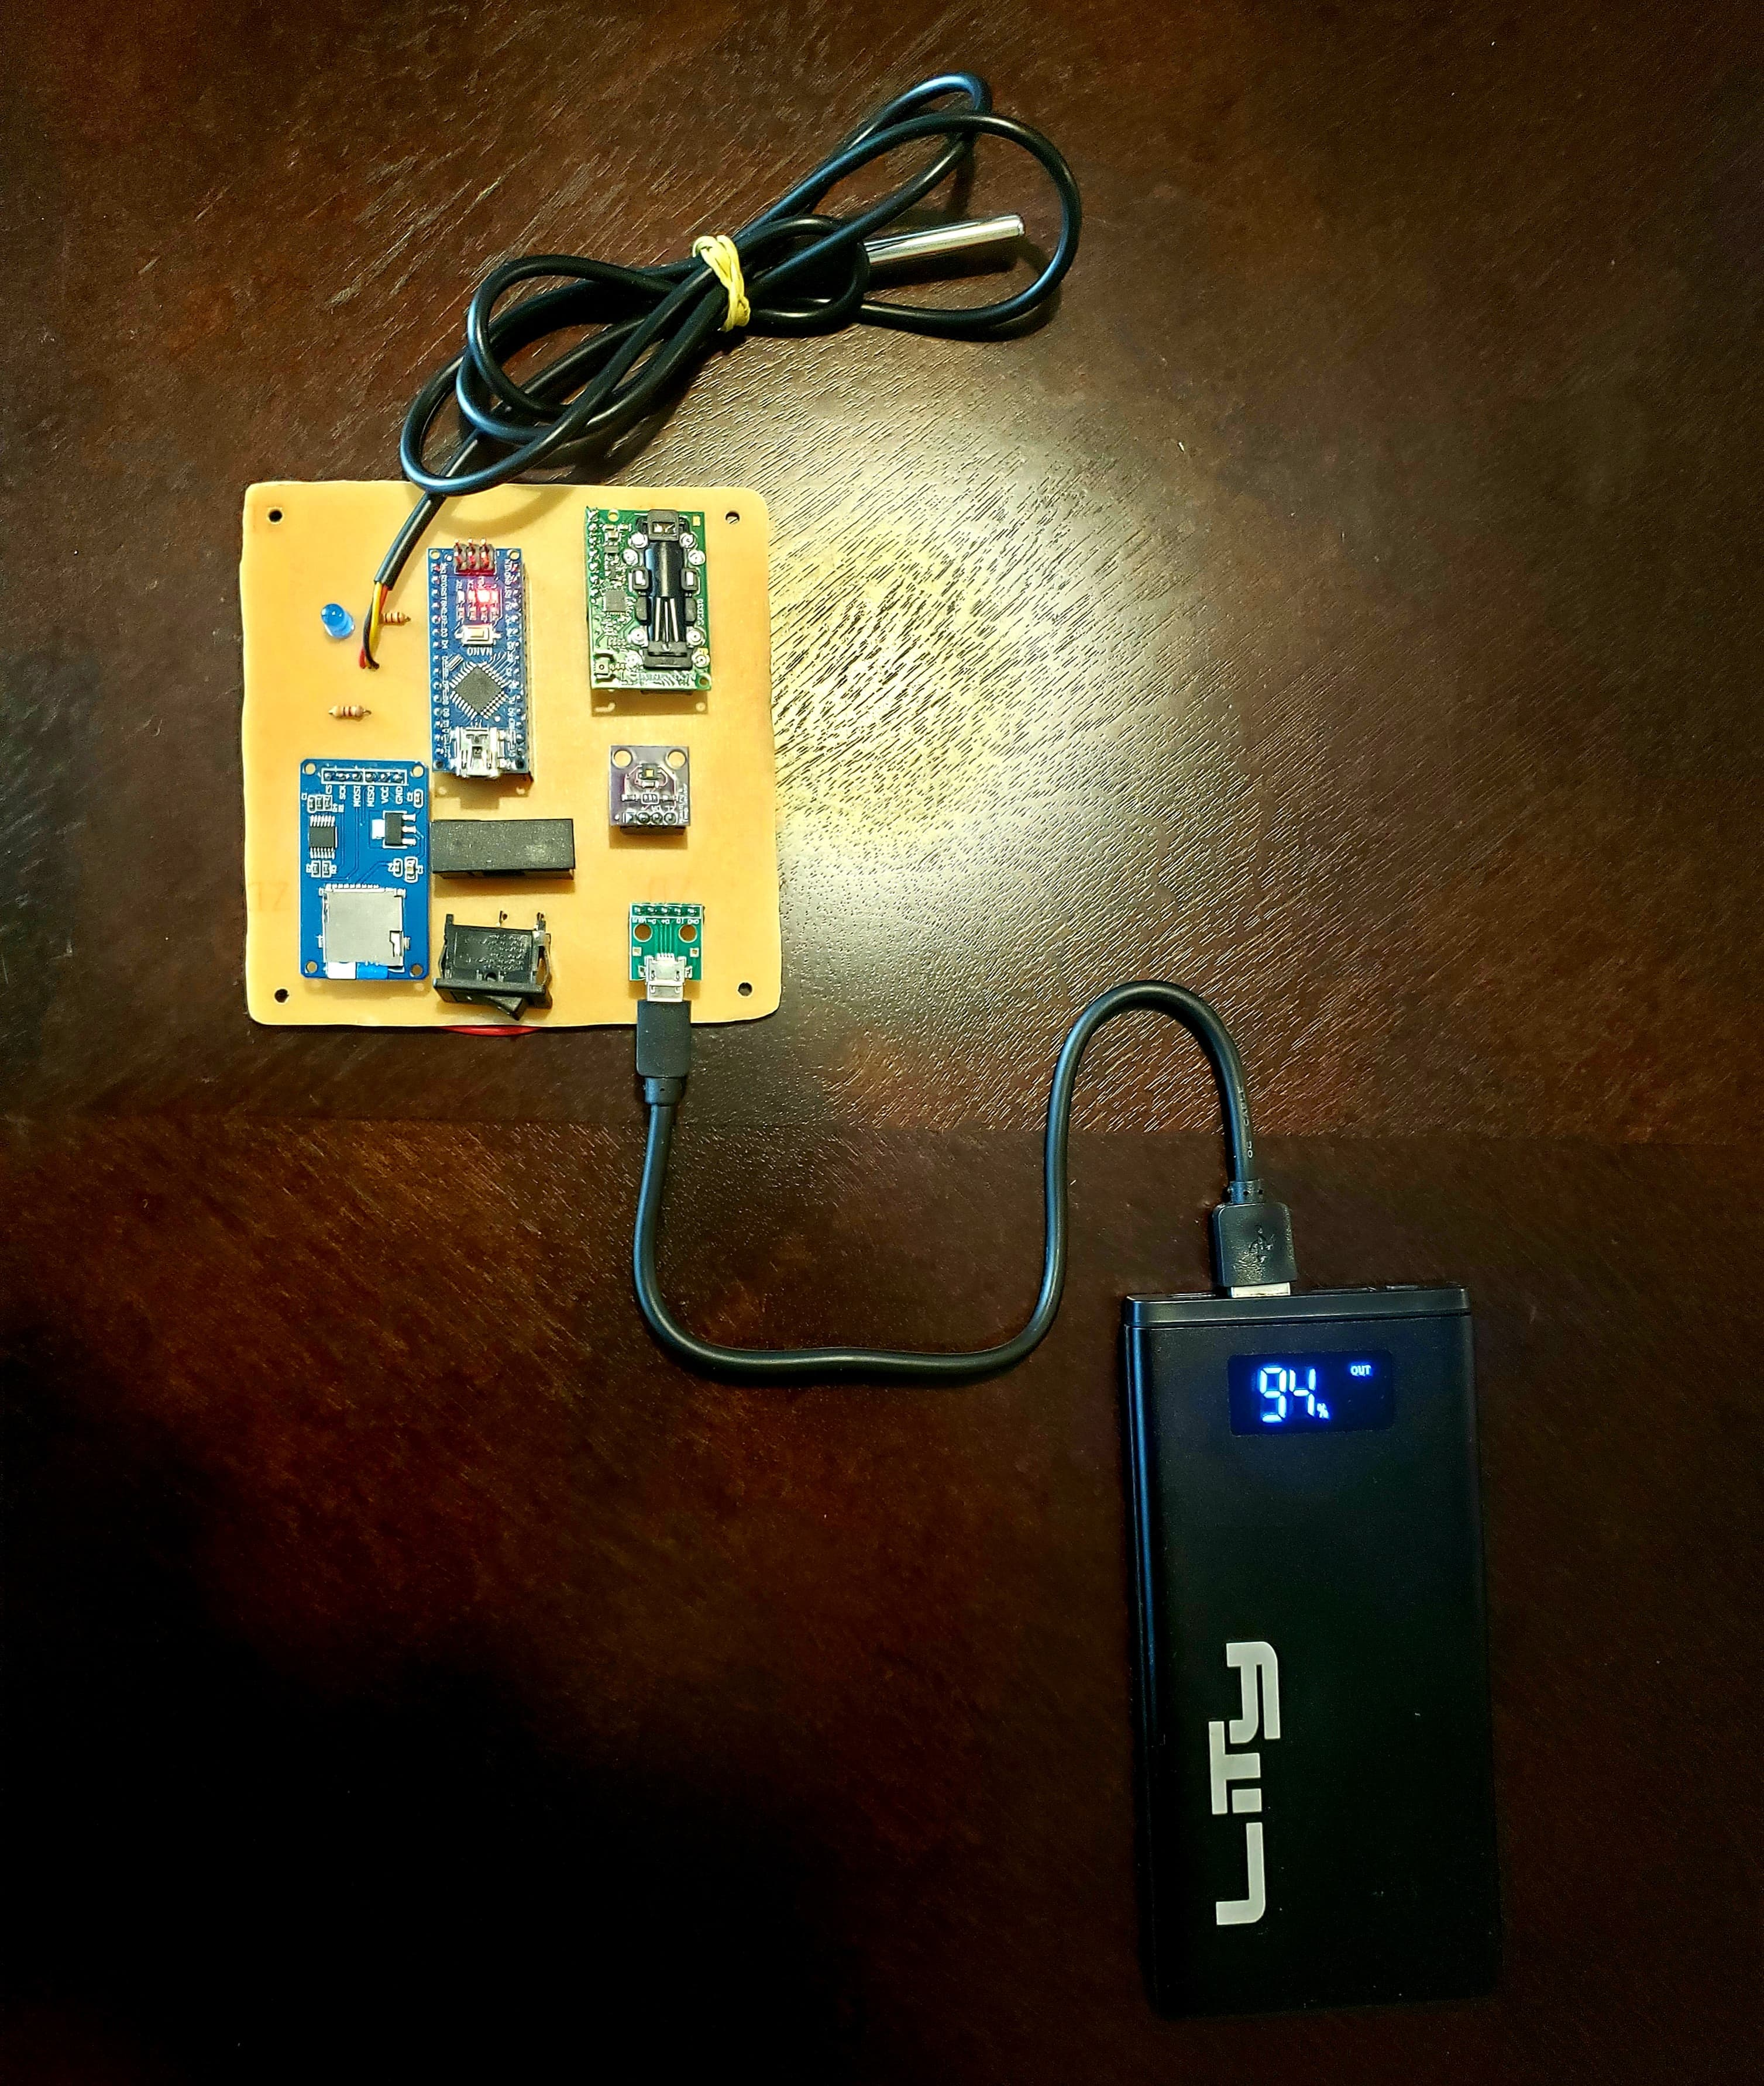
\includegraphics[width=0.60\linewidth]{Imagens/PCB_Conforto.jpeg}
    \smallcaption{Fonte: Autor}
    \label{fig:PCB_conforto}
\end{figure}

\begin{figure}[!htb]
\centering
    \caption{\textit{PCB} do Kit Pressão}
    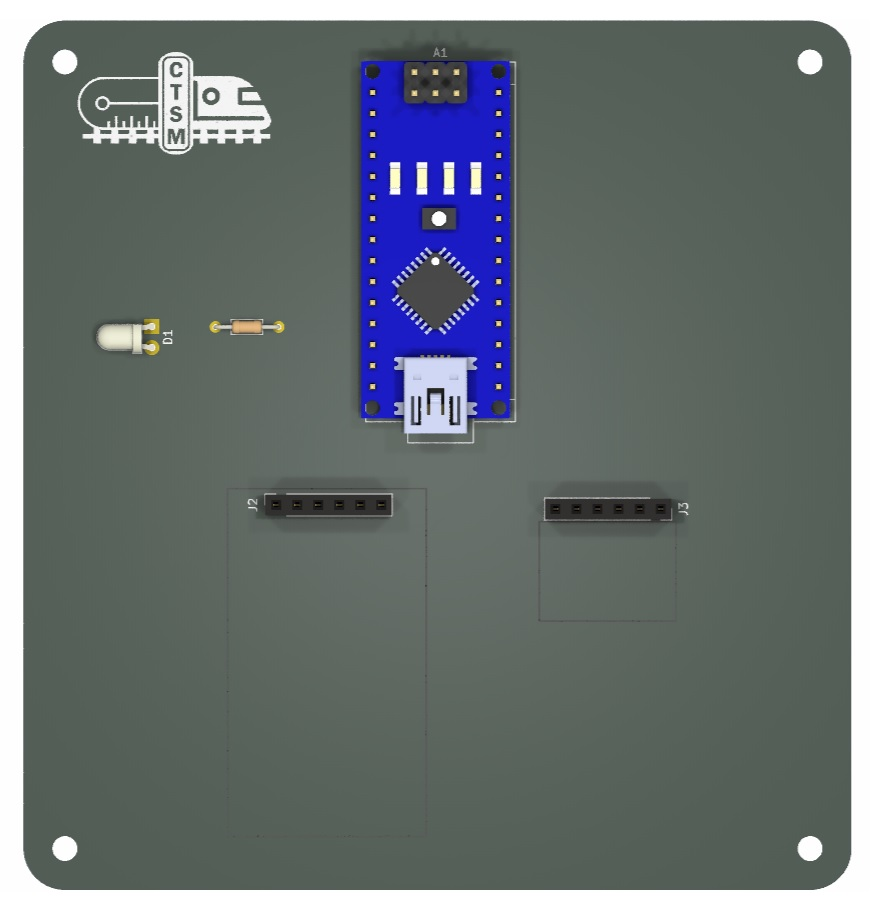
\includegraphics[width=0.50\linewidth]{Imagens/PCB_Pressao.jpg}
    \smallcaption{Fonte: Autor}
    \label{fig:PCB_Pressao}
\end{figure}


Um ponto relevante a se comentar diz respeito à \textit{PCB} do Kit Pressão. Devido à alguns imprevistos, a \textit{PCB} deste kit não estava pronta a tempo da visita marcada com o Metrô de São Paulo para realização das medições. Visto que os dados de pressão devem ser coletados simultaneamente com os de umidade para execução correta dos cálculos de pressão absoluta, tornou-se imprescindível realizar esta medição no dia definido, sob risco de atrasar uma coleta que teria de ser remarcada, o que poderia afetar negativamente o cronograma do grupo. Assim, a \textit{PCB} em questão acabou por não ser produzida, visto que as medições já haviam seguido corretamente apenas com o uso da \textit{protoboard}, situação longe do ideal, mas que mesmo assim conseguiu ser executada com sucesso pelo grupo. Este caso será apresentado e melhor exemplificado também na seção \ref{instruvagao}.


\section{Instrumentação do vagão} \label{instruvagao}

Para a adequada análise do sistema de condicionamento de ar no metrô de São Paulo, foi desenvolvida uma estratégia de instrumentação que visa garantir a máxima precisão na coleta de dados. Após reuniões com o time técnico do Metrô de São Paulo, os pontos de instalação dos sensores foram definidos de forma estratégica, com o intuito de assegurar a melhor qualidade na aquisição de dados, essencial para o sucesso da pesquisa, mas também levando em consideração as limitações impostas ao grupo de modo a não prejudicar os usuários do serviço.

A respeito das reuniões em questão, é valido também comentar sobre as visitas que ocorreram por parte do grupo ao pátio, e o que sucedeu em cada uma delas. A primeira ocorreu no dia dezenove de julho de 2024, onde o grupo teve um primeiro contato com todo o ambiente do Metrô de São Paulo, além de conhecer os sistemas mais internos do carro e uma unidade de ar condicionado muito similar à presente no carro selecionado para o estudo, de modo também a já elencar possíveis posicionamentos para os kits de coleta de dados. Entretanto, como o formato final das \textit{PCBs} não estava definido, estas primeiras ideias tiveram de ser alteradas. Depois, com estas informações, o grupo manteve contato constante com a equipe do Metrô, que, sempre muito prestativa, auxiliou a sanar inúmeras dúvidas.

A próxima visita ocorreu no dia 23 de outubro deste ano. Neste dia, a equipe do Metrô retirou de circulação o conjunto de material rodante L41, Figura \ref{fig:metrol41}, que foi preparado no pátio Jabaquara para o grupo. Por recomendação dos metroviários, analisamos as possibilidades no carro de número 2, classificado como L412, o que permitiu ao grupo uma ideia certeira de onde posicionar as \textit{PCBs}, pois o carro utilizado para as coletas de fato, enquanto que não o mesmo, é idêntico a este modelo. Neste momento, em posse das \textit{PCBs} do Kit Conforto, o grupo realizou uma análise mais precisa dos locais à se instalar os Kits, sempre com a supervisão e recomendações da equipe.

\begin{figure}[!htb]
\centering
    \caption{Material Rodante L41, estacionado no Pátio Jabaquara}
    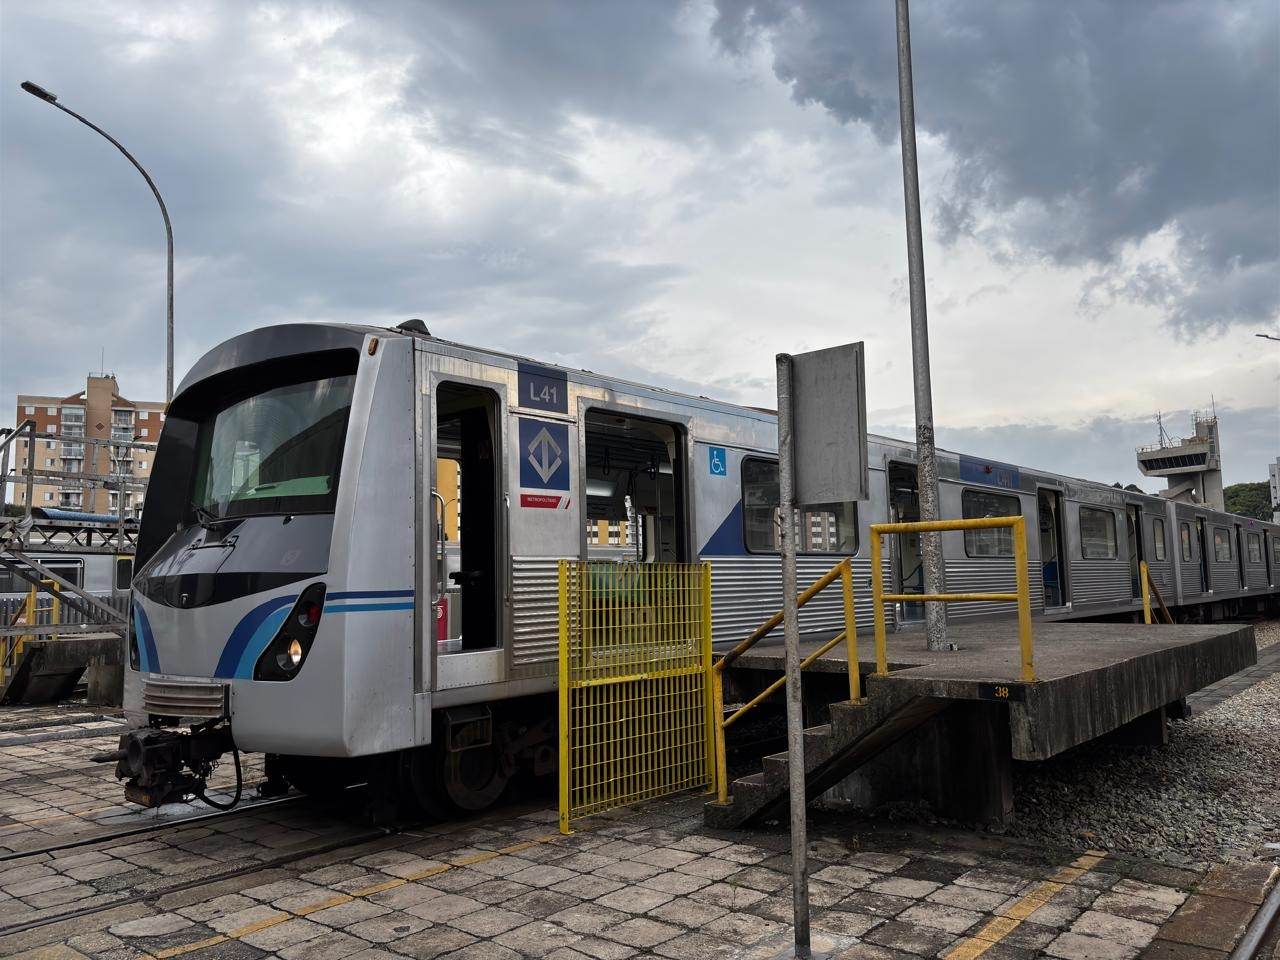
\includegraphics[width=0.60\linewidth]{Imagens/metrol41.jpg}
    \smallcaption{Fonte: Autor}
    \label{fig:metrol41}
\end{figure}

A terceira e última visita ocorreu no dia 25 de outubro do mesmo ano. Aqui, os integrantes do grupo chegaram ao mesmo pátio às quinze horas, com o intuito de preparar os Kits no carro de número 2 do material L28, denominado de L282, Figura \ref{fig:metrol282}, escolhido pela equipe do Metrô, até as dezessete horas, visto que o conjunto foi retirado logo no início da tarde, onde há menor movimento, mas deve ser devolvido à via ao fim da tarde, onde se inicia um dos horários de pico do dia. Com o auxílio dos metroviários e as informações definidas na visita anterior, além de materiais como tesoura, fita adesiva dupla-face, abraçadeiras de nylon e suportes de papelão rígido para as \textit{PCBs}, presentes na Figura \ref{fig:matusados}, os Kits e seus respectivos \textit{Power Banks} foram instalados da maneira esperada no carro. 

\begin{figure}[!htp] 
    \centering
    \begin{minipage}{0.45\textwidth}
        \caption{Carro de número 2 do material L28}
        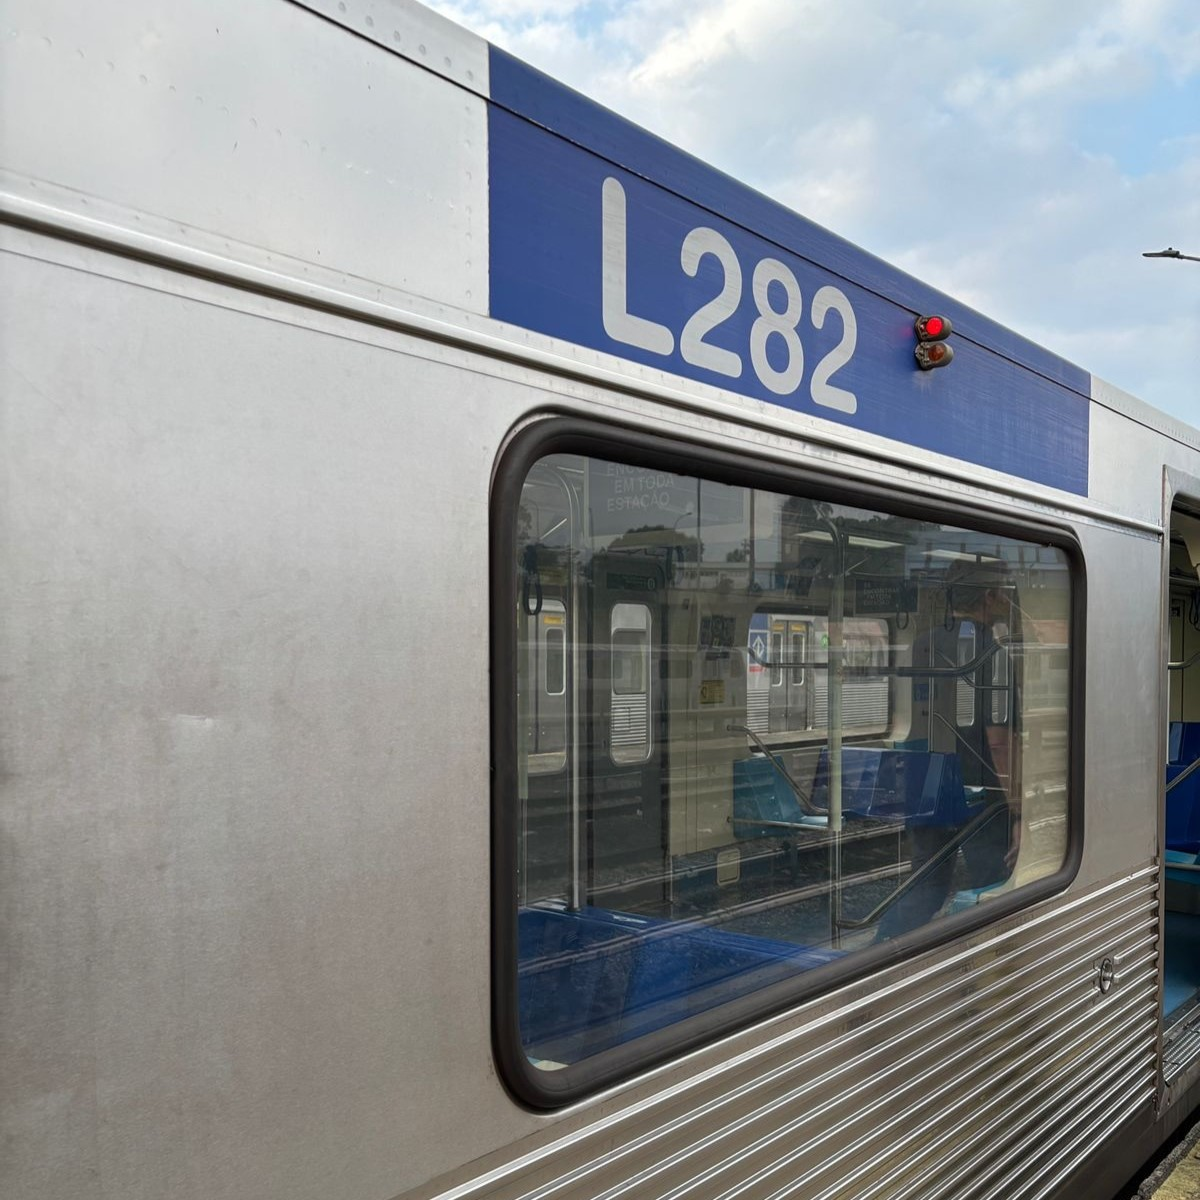
\includegraphics[width=\linewidth, height=7.5cm]{Imagens/metrol282.jpg} 
        \smallcaption{Fonte: Autor}
        \label{fig:metrol282}
    \end{minipage}\hfill
    \begin{minipage}{0.45\textwidth}
        \caption{Materiais utilizados para fixação dos Kits no carro}
        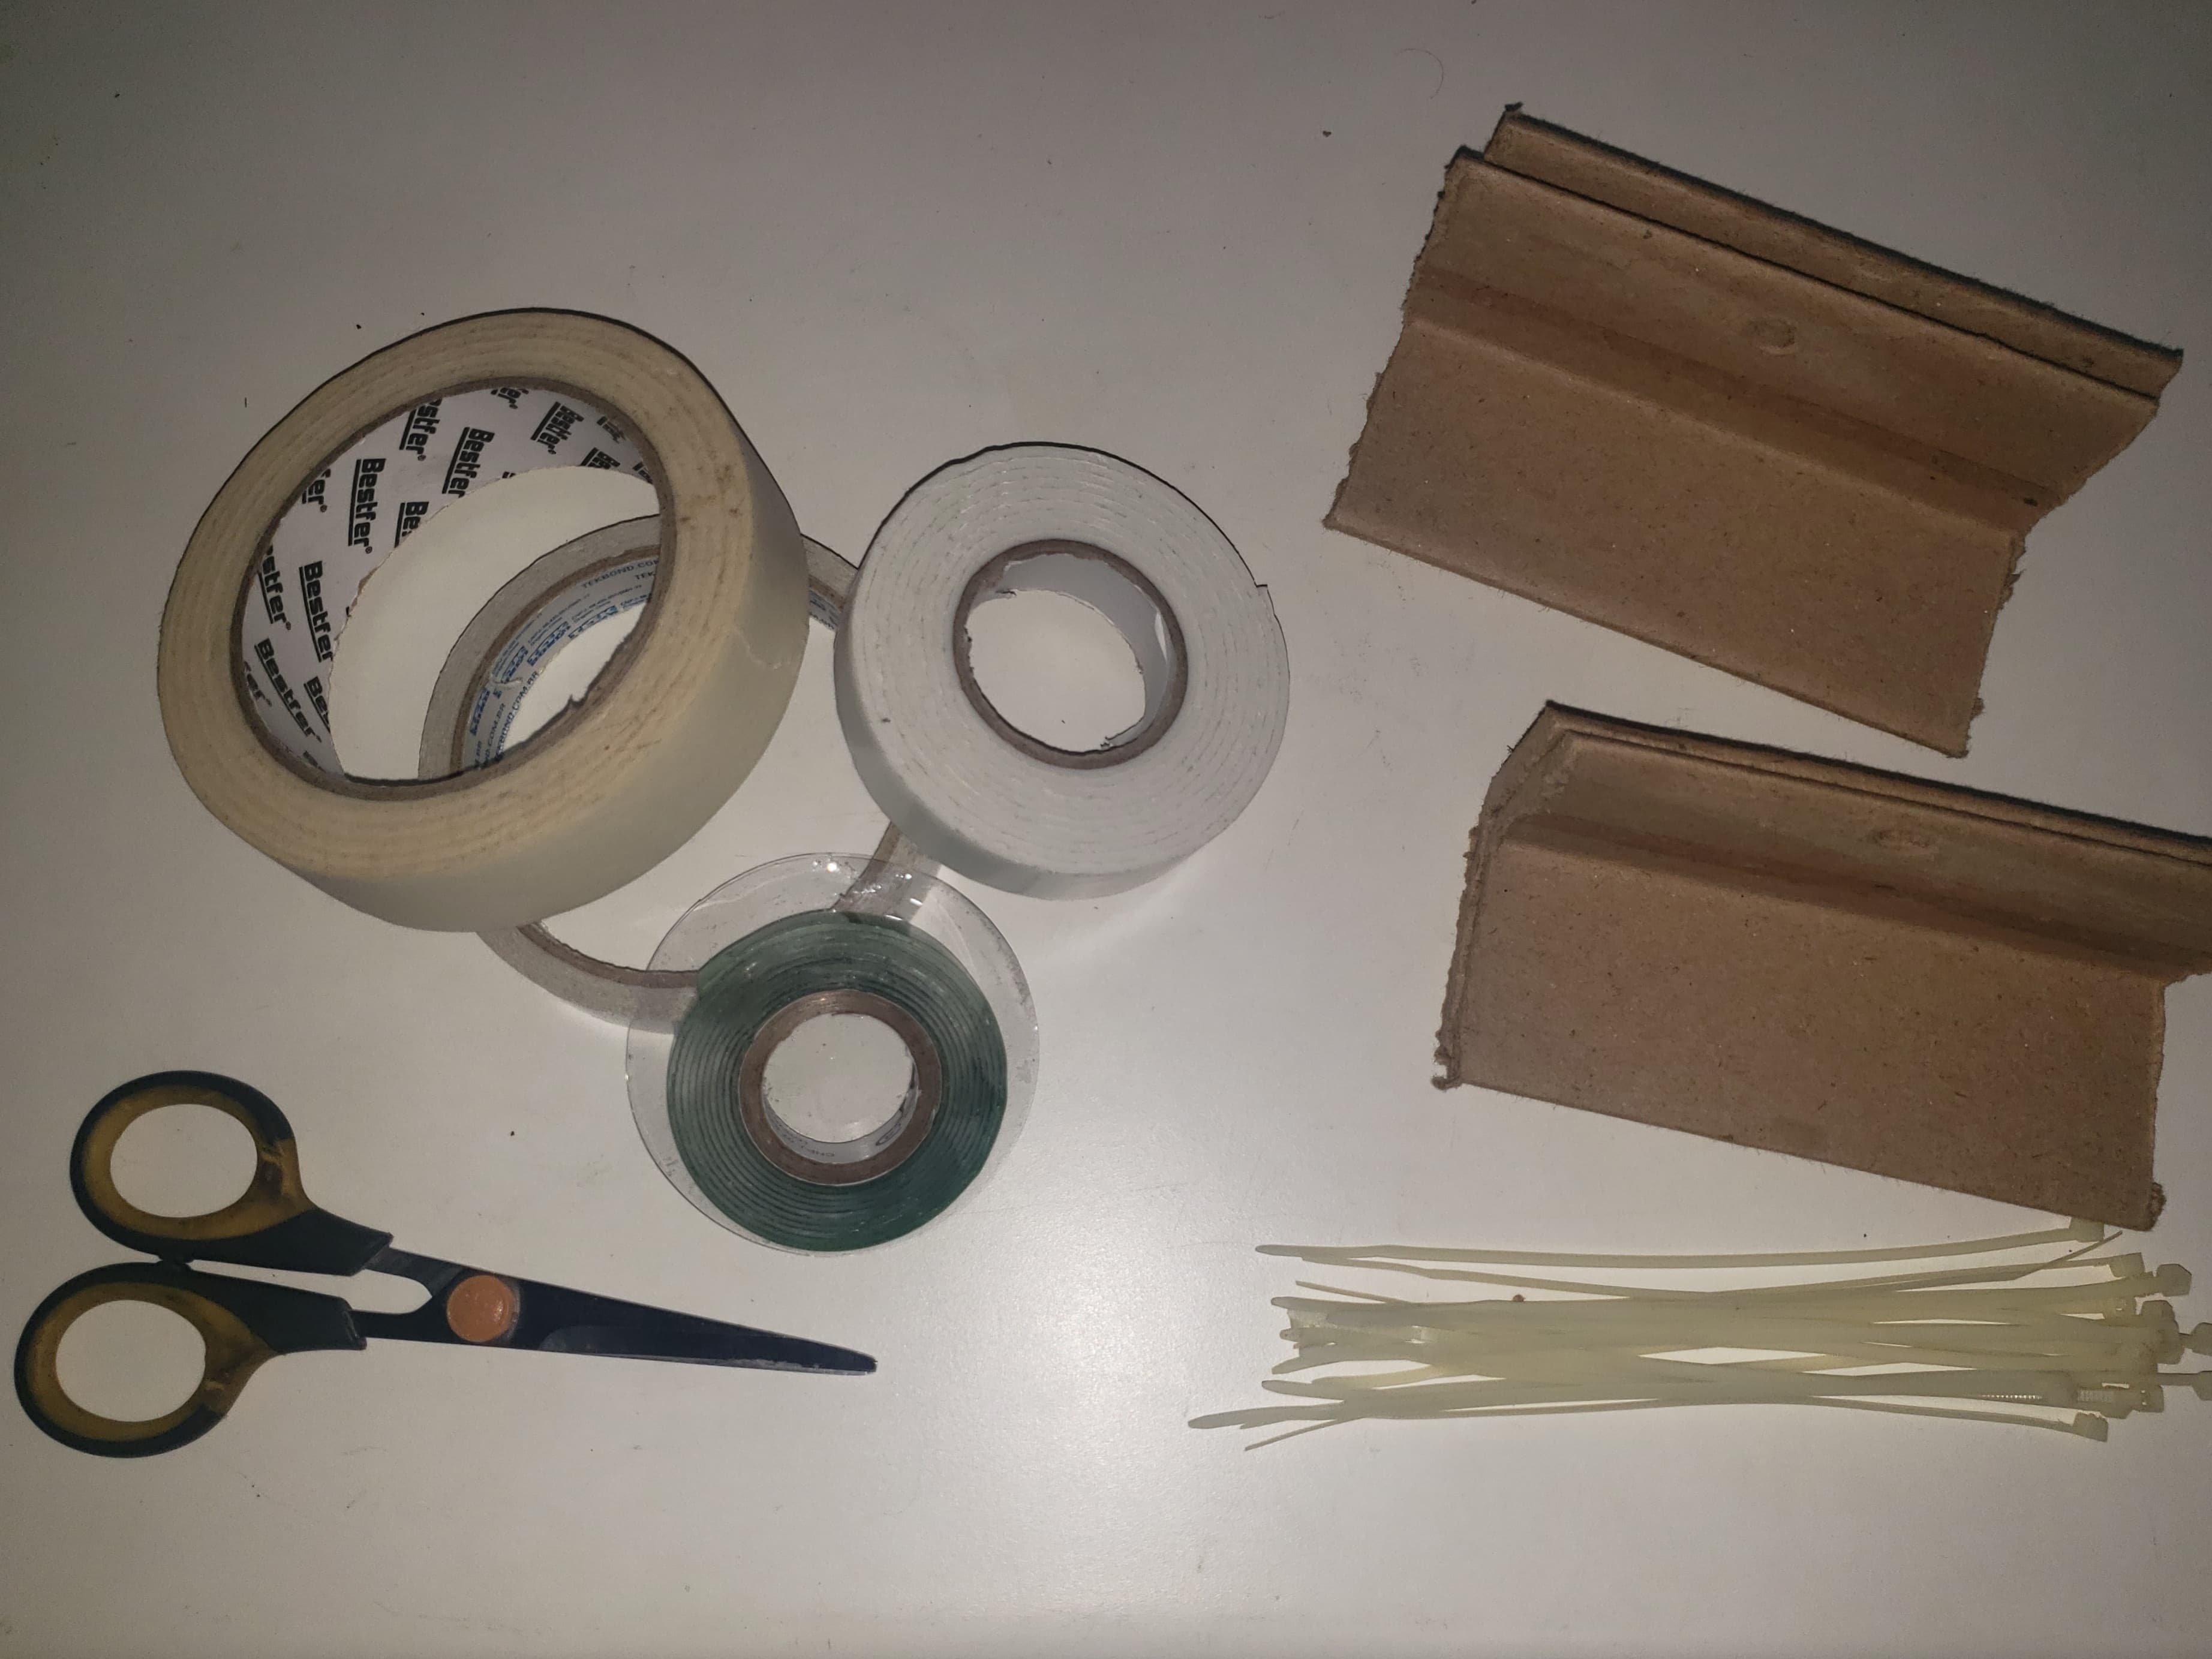
\includegraphics[width=\linewidth, height=7.5cm]{Imagens/matusados.jpeg} 
        \smallcaption{Fonte: Autor}
        \label{fig:matusados}
    \end{minipage}
\end{figure}

A campanha de medições foi efetuada em um único dia, com coletas realizadas a partir das 16 horas e 44 minutos do dia 25 de outubro de 2024, momento onde todos os kits foram ligados de modo a dar início à suas rotinas de calibração e também já coletando informações sobre o carro vazio, até as 20 horas e 54 minutos do mesmo dia, totalizando 4 horas e 10 minutos de aquisição de dados. É valido comentar também que a primeira estação visitada foi o Jabaquara, às 16 horas e 53 minutos, pois há uma certa distância entre o pátio e a estação que levam o mesmo nome, além de que o percurso completo de ida e volta, partindo e retornando ao Jabaquara conforme o Metrô voltava ao atingir a estação Tucuruvi, foi realizado um total de 3 vezes.

Esse período de coleta foi definido estrategicamente para que os dados fossem capturados em diferentes momentos de operação do metrô, abrangendo tanto horários de menor fluxo de passageiros, quanto horários de pico com maior lotação. Essa abordagem permitirá uma análise mais robusta e detalhada, uma vez que o comportamento do sistema de climatização pode variar de acordo com a densidade de ocupação dos vagões. A coleta de dados em horários mais vazios e em horários de pico fornecerá uma visão mais ampla sobre o desempenho do sistema em condições operacionais variadas, o que é essencial para avaliar a eficiência do controle térmico e da qualidade do ar em diferentes cenários de demanda, garantindo assim uma boa assertividade na análise dos dados.

Foram utilizados ao todo quatro kits de medição, distribuídos entre um kit para pressão e três kits para conforto. Os três kits iguais, equipados com sensores de temperatura, concentração de dióxido de carbono (${CO}_{2}$) e umidade relativa do ar, foram utilizados para realizar medições em pontos distintos do vagão, priorizando a análise da circulação de ar, sendo instalados em pontos próximos ao insuflamento e à exaustão, marcados em verde na Figura \ref{fig:metodo_de_medicao}, com o objetivo de capturar dados diretamente relacionados ao fluxo de ar-condicionado. Estas PCBs foram posicionadas em áreas estratégicas, sendo elas:

\begin{itemize}[label=\arabic*.]
    \item Televisão próxima ao insuflamento central do carro, geralmente considerado mais gelado pela equipe e usuários do Metrô. Apresentada na Figura \ref{fig:kittv};
    \item Apoiada em uma barra de apoio ao lado das portas, próxima a um dos pontos de exaustão do ar e margeando a zona afetada pelo insuflamento mencionado no item a. Apresentada na Figura \ref{fig:kitporta};
    \item Base de uma janela ao fundo do carro, sendo este um ponto secundário também de insuflamento, mas de menor influência. Apresentada na Figura \ref{fig:kitjanela}.
\end{itemize}

\begin{figure}[!htb] 
    \centering
    \begin{minipage}{0.45\textwidth}
        \caption{Kit Conforto instalado na Televisão do Metrô}
        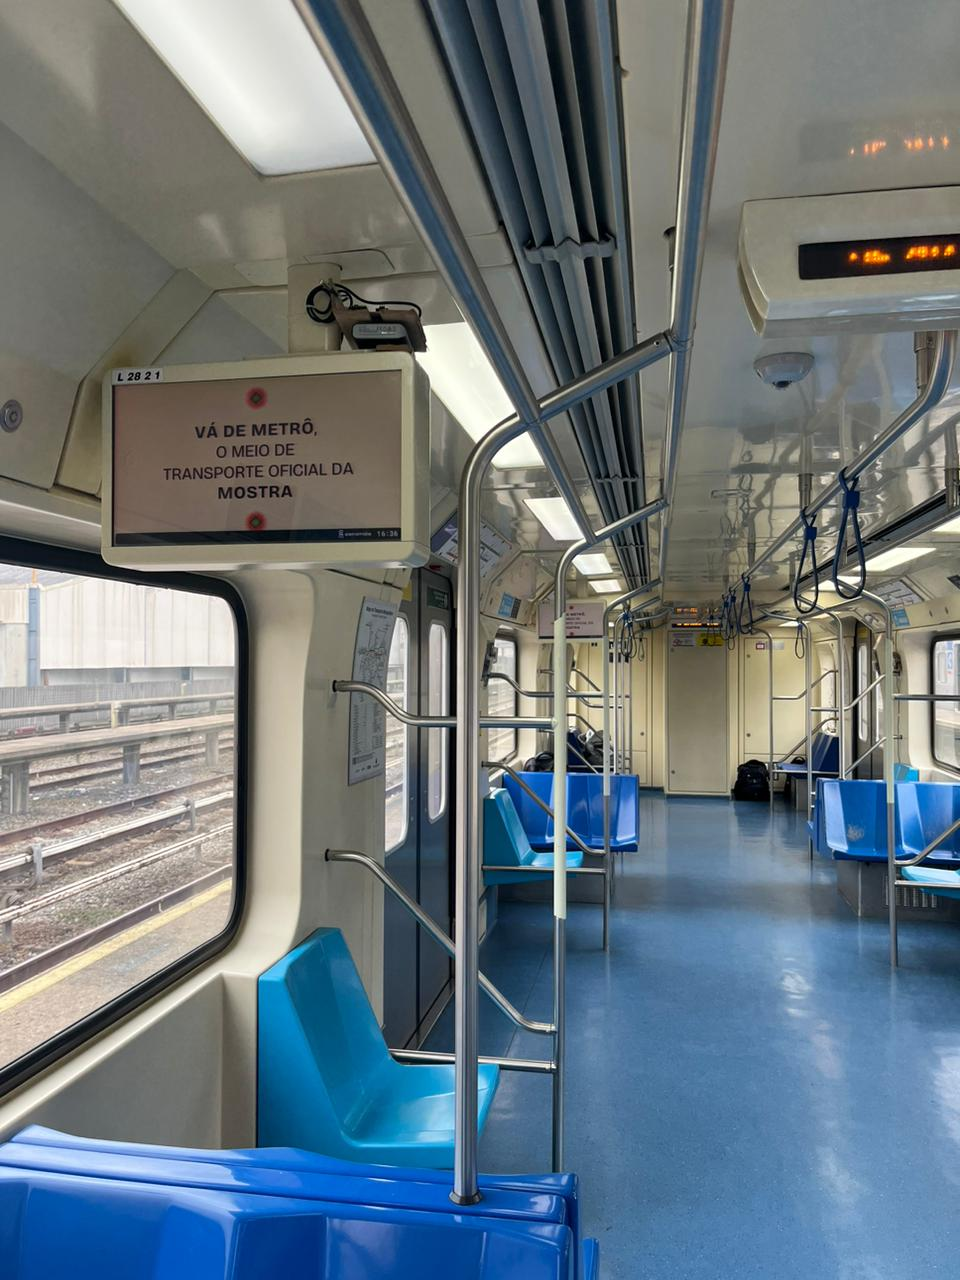
\includegraphics[width=\linewidth, height=9.5cm]{Imagens/kittv.jpeg} 
        \smallcaption{Fonte: Autor}
        \label{fig:kittv}
    \end{minipage}\hfill
    \begin{minipage}{0.45\textwidth}
        \caption{Kit Conforto instalado acima de uma barra de apoio}
        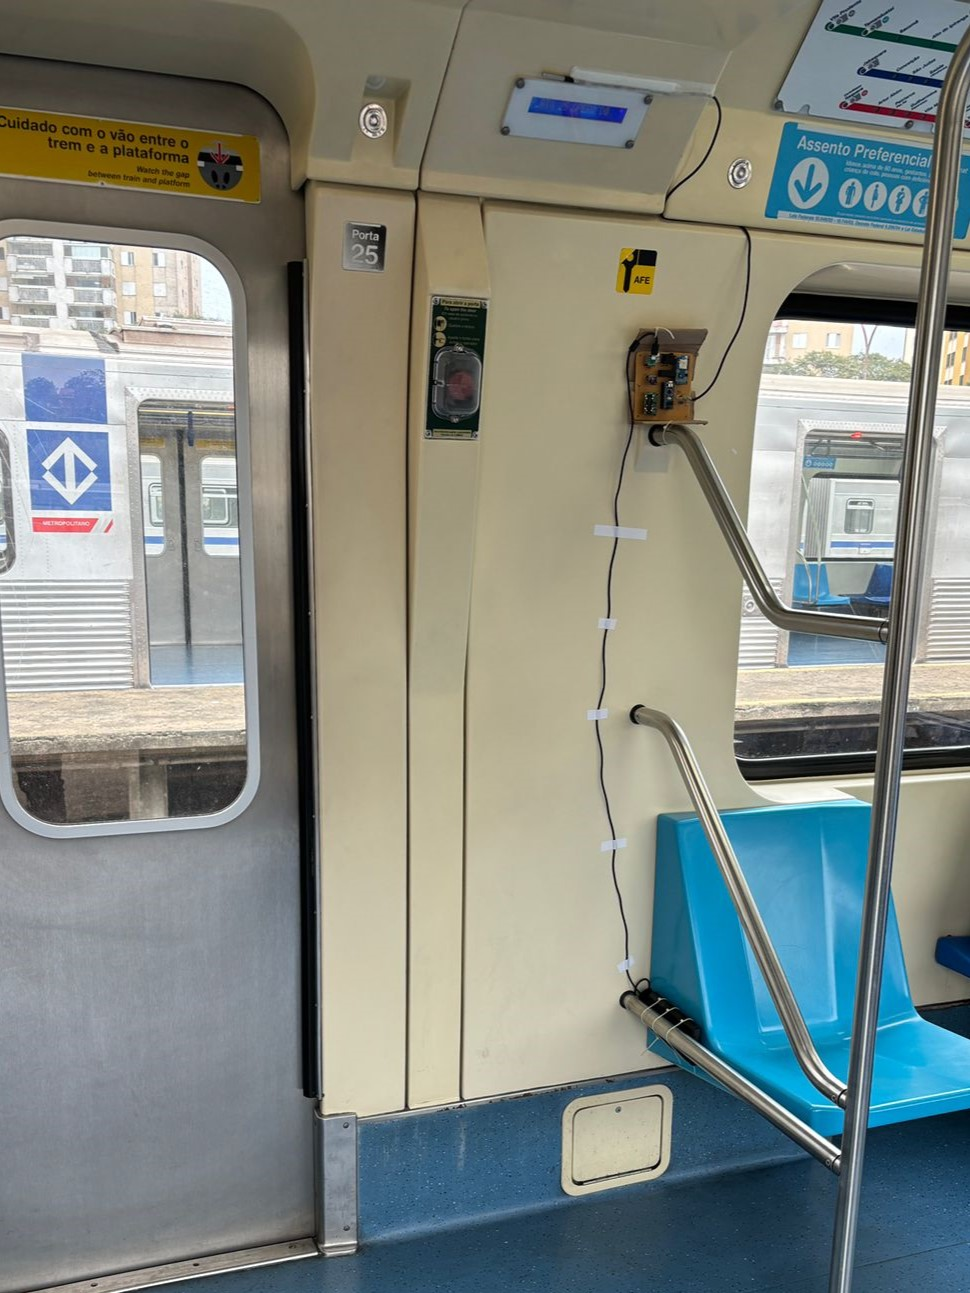
\includegraphics[width=\linewidth, height=9.5cm]{Imagens/kitporta.jpeg} 
        \smallcaption{Fonte: Autor}
        \label{fig:kitporta}
    \end{minipage}
\end{figure}

\begin{figure}[!htb]
\centering
    \caption{Kits Conforto e Pressão instalados na janela ao fundo do carro}
    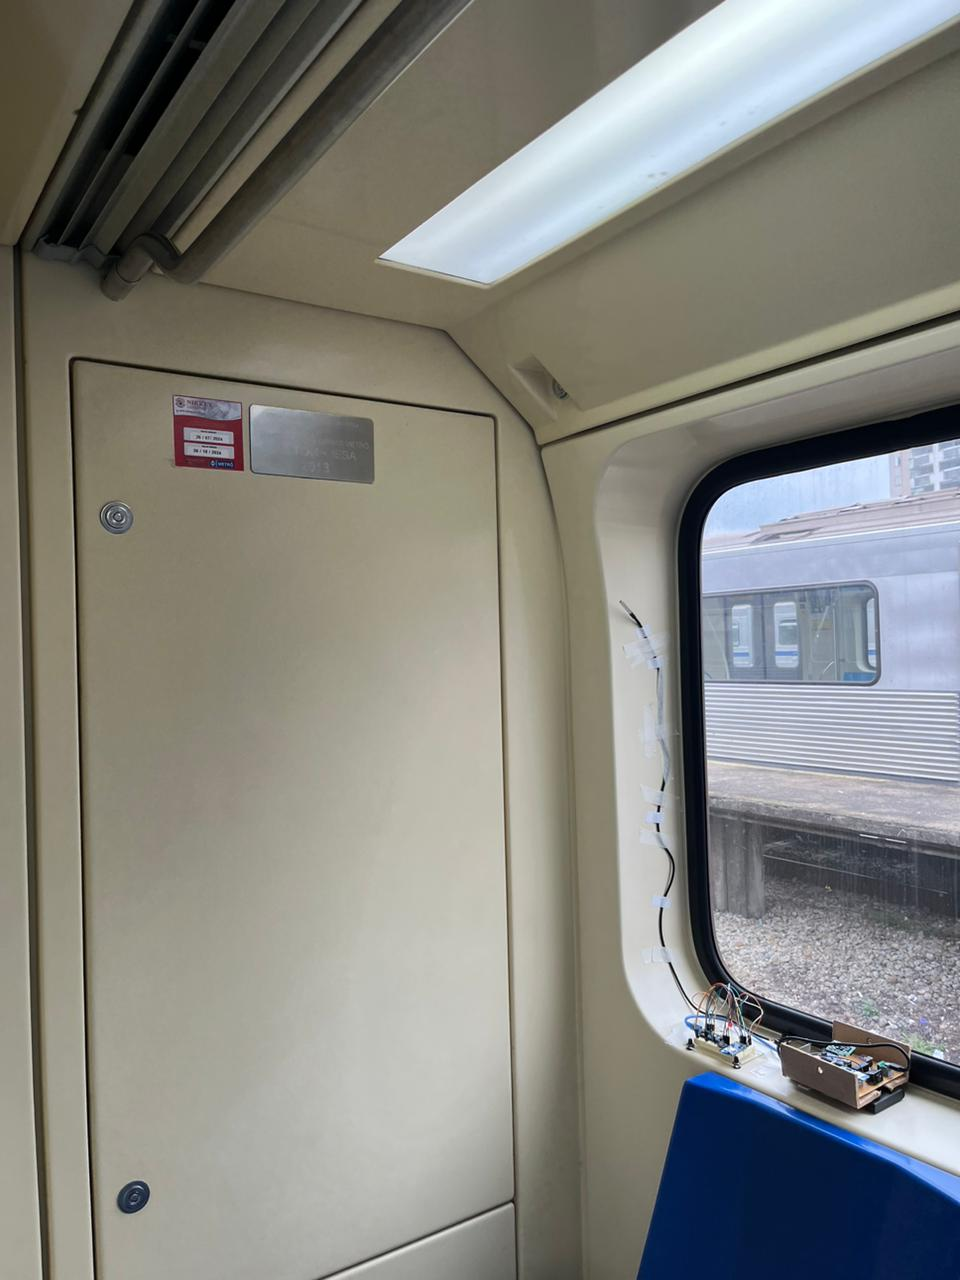
\includegraphics[width=0.50\linewidth]{Imagens/kitjanela.jpeg}
    \smallcaption{Fonte: Autor}
    \label{fig:kitjanela}
\end{figure}
\newpage

É válido comentar que o Kit Conforto da janela realizou as medições em uma posição ligeiramente inferior aos demais. A intenção é comparar as condições ambientais próximas ao insuflamento e à exaustão com as medições feitas em uma zona mais neutra, onde o ar já está em circulação pelo ambiente. Essa comparação permitirá uma avaliação mais detalhada da distribuição de temperatura, umidade e concentração de ${CO}_{2}$ dentro do vagão, fornecendo novas ideias sobre a eficiência do sistema de climatização em diferentes áreas do espaço.

O Kit Pressão, por sua vez, foi instalado no mesmo local que o Kit Conforto ao fundo do carro, conforme ilustrado em amarelo na Figura \ref{fig:metodo_de_medicao} e visto também nas Figuras \ref{fig:kitjanela} e, com mais detalhes, \ref{fig:kitjanelazoom}. Este sensor tem a função de medir a pressão barométrica local. A escolha desse posicionamento se justifica pela praticidade no momento da instalação e fixação do kit, além de outras duas questões técnicas. A primeira está ligada simplesmente a quantidade de saídas \textit{USB} encontradas nos \textit{Power Banks}, já que o banco de baterias que possui duas destas saídas foi o colocado na janela. A segunda questão diz respeito à construção deste kit. Como mencionado na seção \ref{Proto}, a PCB para esta placa não ficou pronta na data esperada, tornando então necessário o posicionamento mais simples possível para este kit visto que a \textit{protoboard} não apresenta caráter de produto final, isto é, locais mais complexos resultariam em possíveis problemas causados pelas conexões via \textit{jumper} expostas, além de sua facilidade de desconexão acidental, ocasionada por toque não intencionado de algum usuário do Metrô, ou até mesmo a simples vibração enfrentada pelo carro.

\begin{figure}[!htb]
\centering
    \caption{Visão com maior detalhe dos Kits Conforto e Pressão instalados na janela ao fundo do carro}
    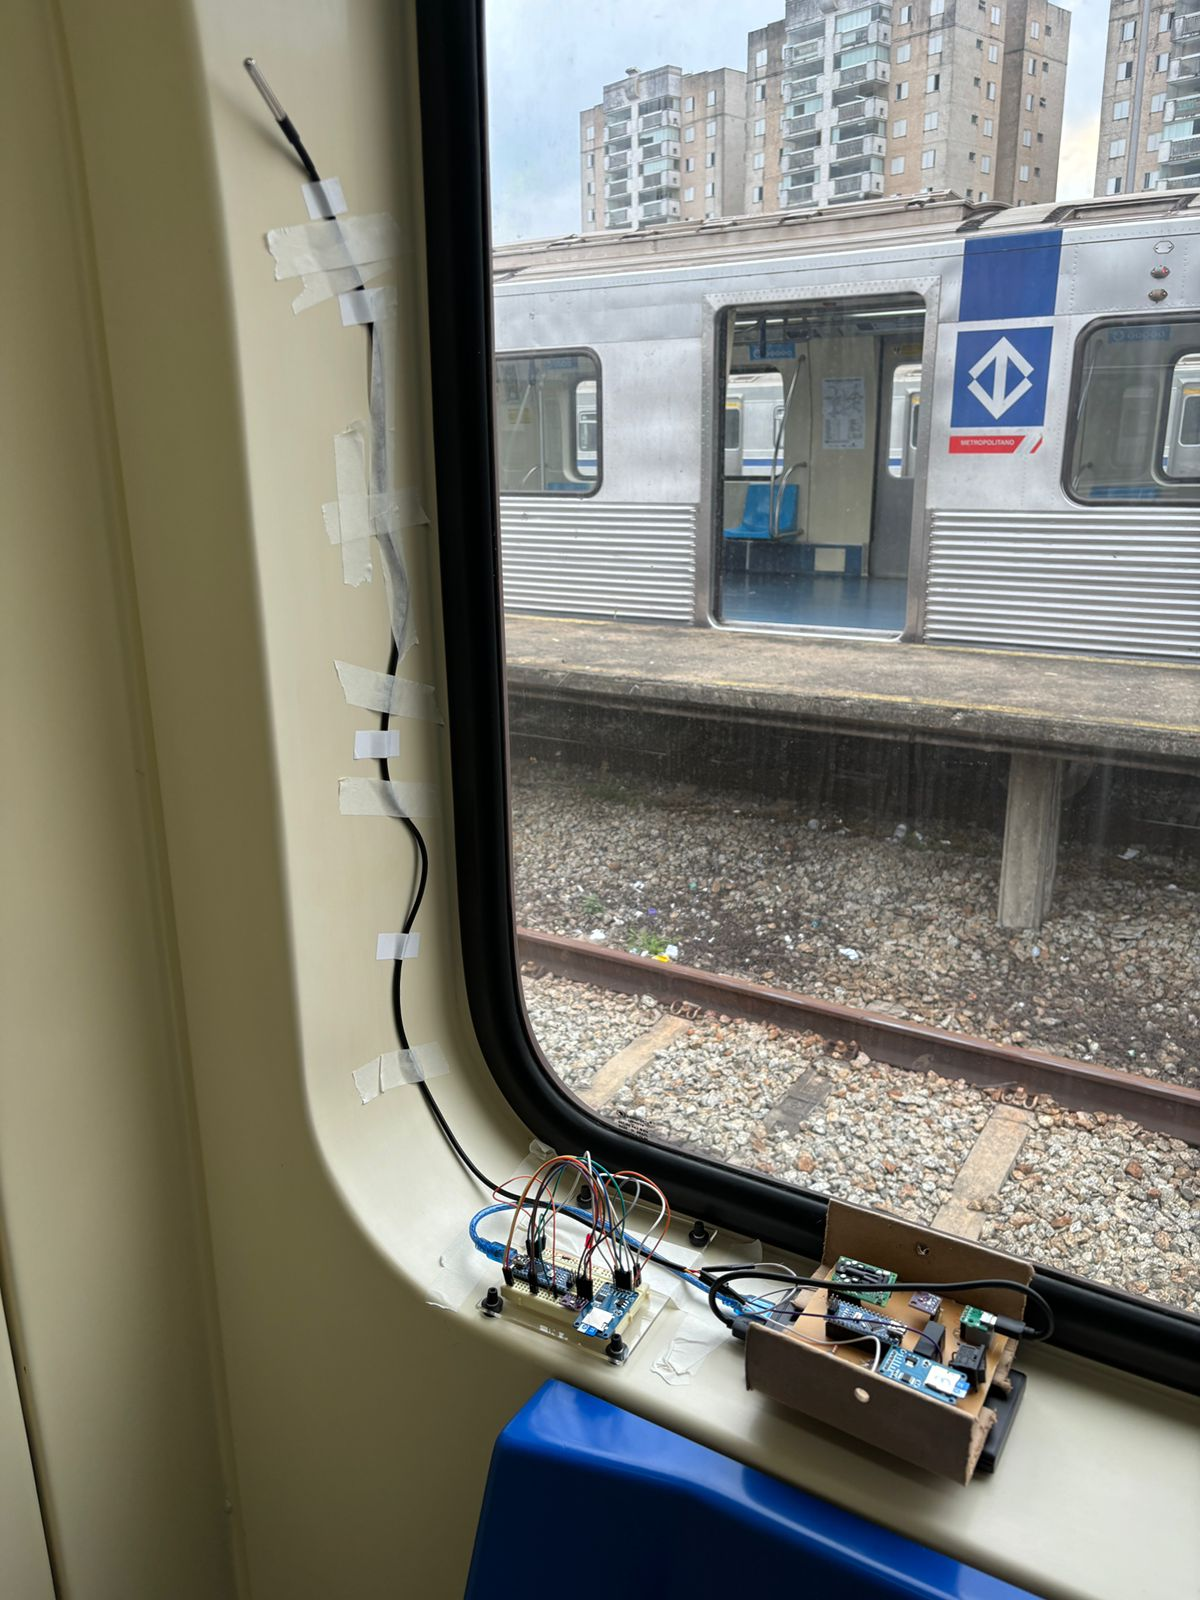
\includegraphics[width=0.50\linewidth]{Imagens/kitjanelazoom.jpeg}
    \smallcaption{Fonte: Autor}
    \label{fig:kitjanelazoom}
\end{figure}

Dados estes apontamentos, é possível dizer que a abordagem metodológica escolhida pelo grupo, validada pelo time técnico do Metrô de São Paulo, visa proporcionar uma visão detalhada e suficientemente precisa das condições de operação do sistema de ar-condicionado, mesmo em condições não ideais como a exposta com o caso do Kit Pressão, contribuindo para otimizar o conforto dos passageiros e a eficiência energética dos sistemas de climatização. 

\section{Dados fornecidos pelo Metrô de São Paulo}

Os dados recebidos através da equipe do Metrô de São Paulo são essenciais para o estudo realizado, por possibilitarem uma contextualização das condições atuais do sistema. Além disso, são dados necessários para a realização dos cálculos teóricos, desenvolvimento das simulações fluidodinâmicas e para a análise estatística dos dados. Nesse sentido, seria inviável realizar modelagens e cálculos precisamente a partir de dados que não refletem diretamente as condições atuais do sistema de ar-condicionado.

Visando fundamentar o estudo realizado, foram recebidos dados diretamente do Metrô de São Paulo, que permitiram uma análise mais aprofundada do problema. A equipe responsável forneceu a temperatura de exaustão e insuflamento do vagão, o peso dos carros e as reclamações dos passageiros direcionadas ao funcionamento do Metrô, além de esquemáticos e desenhos do vagão. 

\subsection{Peso dos Carros} 

    A medição de peso nos carros do Metrô de São Paulo é efetuada através das bolsas de ar do sistema de suspensão, localizadas nos “truques” (conjunto de rodas) dos vagões. As bolsas ajustam a altura do vagão, ajustando o nível conforme o peso a ser transportado. O sistema pneumático, alimentado por um compressor, é responsável por fornecer o ar comprimido para as bolsas, que por sua vez são controladas por válvulas niveladoras. Essas válvulas mantêm a pressão balanceada nas bolsas. Por sua vez, os transdutores de pressão presentes no sistema pneumático possibilitam direcionar os dados para o sistema eletrônico do trem.
    
    A pressão nas bolsas de ar de vagão está diretamente ligada ao número de passageiros. Com isso, a pressão é convertida para um valor em toneladas, o que pode ser convertido posteriormente para um número aproximado de pessoas presentes no carro. Exemplificando, a partir do peso em toneladas do vagão, pode-se estimar o número de pessoas presente no vagão em determinado horário, por exemplo, uma pressão correspondente a duas toneladas de peso indica que existem aproximadamente 30 pessoas no vagão, considerando um peso médio por pessoa de 70 kg.
    
    No contexto apresentado, o peso do vagão foi utilizado para estimar o número aproximado de pessoas, visto que a equipe do Metrô de SP não possuía a informação do número exato de pessoas por carro, sendo uma informação valiosa para o tratamento e análise de dados realizados. É importante mencionar que, por se tratar de um conteúdo confidencial, não foi permitida a divulgação do diagrama do sistema pneumático do metrô.
    
    Dessa maneira, foram recebidas planilhas através da equipe do Metrô de SP contendo o peso dos carros da frota L medido pelo sistema descrito anteriormente \cite{metrosp2024}. Como é possível observar na Figura \ref{fig:Peso_Carros}, o vagão número 5 passou de 12 toneladas para 9 toneladas, ou seja, aproximadamente 43 pessoas saíram na estação, considerando um peso médio de pessoa de 70 kg.
    
    \begin{figure}[!htb]
    \centering
    \caption{Peso em Cada Vagão da frota L}
    \includegraphics[width=1\linewidth]{Imagens/Peso_Carros.png}
    \smallcaption{Fonte: \textcite{metrosp2024}}
    \label{fig:Peso_Carros}
    \end{figure}

\subsection{Temperatura interna e externa do carro} 
    
    Foram recebidos dados dos sensores de temperaturas já presentes no carro, localizados entre o salão e o filtro, sendo no caso, a temperatura de exaustão. Essas informações foram utilizadas na análise, permitindo a construção de gráficos e tratamento de dados. Além disso, foi utilizada de maneira comparativa, visando validar o funcionamento dos sensores de temperatura instalados para o sensoriamento \cite{metrosp2024}. 

    O Metrô de São Paulo possui dois sensores de temperatura instalados, um de exaustão, localizado entre o salão e o filtro do ar condicionado e outro fixado na parte externa do vagão. Dessa maneira, pode-se dizer que o sensor interno não representa de maneira verdadeira a temperatura na área em que as pessoas circulam, não oferecendo dados muito precisos do sistema a ser estudado, apenas servindo de referência para o estudo.

    Os sensores utilizados pela empresa são sensores de temperatura \textit{E52-E} que podem ser observados na Figura \ref{fig:Sensores_Metro}. Esses sensores possuem uma vasta gama de opções para o alojamento, facilitando montagem e ligação. Além disso, possui ótima correspondência de desempenho como controlador térmico. Como é possível observar na Figura \ref{fig:Temperatura_Carros}, é possível ver todas as Temperaturas de exaustão e externa, para cada carro.
    
    
    \begin{figure}[!htb]
    \centering
    \caption{Sensores de Temperatura Utilizados pelo Metrô de SP}
    \includegraphics[width=1\linewidth]{Imagens/Sensor_Metro.jpg}
    \smallcaption{Fonte: \textcite{metrosp2024}}
    \label{fig:Sensores_Metro}
    \end{figure}

    \begin{figure}[!htb]
    \centering
    \caption{Temperatura em Cada Vagão da frota L}
    \includegraphics[width=1\linewidth]{Imagens/Temperatura_Carros.png}
    \smallcaption{Fonte: \textcite{metrosp2024}}
    \label{fig:Temperatura_Carros}
    \end{figure}

\subsection{Reclamações dos usuários da frota L}

    As reclamações dos passageiros da frota foram adquiridas através do portal de reclamações do Metrô, no caso, o “SMS-Denúncia” da CPTM, sendo um serviço que possibilita que os passageiros do Metrô denunciem irregularidades ou façam reclamações sobre ocorridos no vagão. Tendo isso em vista, para realizar a denúncia, a pessoa deve descrever o acontecimento, informando a linha, o número do vagão e a estação. 
    
    A equipe do Metrô forneceu planilhas contendo as reclamações referentes ao ar-condicionado realizadas pelos usuários, que possuem dados organizados por dia e horário, natureza da reclamação, número do trem e do carro, além do número da via, como é possível observar na Figura \ref{fig:SMS_Denuncia}. Esses dados foram utilizados no estudo estatístico que, em conjunto com os outros segmentos do trabalho, possibilitou a análise e tratamento de dados, juntamente a proposição  de melhorias \cite{metrosp2024}.
    
\begin{figure}[!htb]
    \centering
    \caption{Trecho da Planilha das Reclamações da frota L}
    \includegraphics[width=1.0\linewidth]{Imagens/SMS_Denuncia.png}
    \smallcaption{Fonte: Autor}
    \label{fig:SMS_Denuncia}
\end{figure}


\subsection{Esquemáticos e desenhos do vagão} 
    
Durante o desenvolvimento do trabalho, foram recebidos desenhos 2D e esquemáticos do metrô e do sistema de ar-condicionado, contendo detalhes técnicos a respeito da geometria e estrutura dos carros e do ar condicionado. Esses documentos são essenciais para a realização de uma análise coesa, tanto dos processos de troca térmica quanto das simulações fluido dinâmicas. A partir dos desenhos 2D recebidos, foram desenvolvidos modelos 3D utilizados para as simulações e para definir a geometria adotada para o vagão. É importante mencionar que, por se tratar de um conteúdo confidencial, não foi permitida a divulgação do material, juntamente com a divulgação das dimensões exatas do vagão.
 

%Explicar os dados que foram fornecidos e como é o o metro ideia de geometria, etc. Explicar como funciona seu sensor de temperatura, peso, e reclamações. Fazer subtópicos.

\section{Conforto Térmico}

Como dito nas premissas do projeto e nas simplificações a \textcite{ASHRAE2009} tem algumas normas que ditam o conforto térmico. O estudo do conforto térmico é importante porque dita a condição em que o ambiente se encontra e avalia, também, como as pessoas percebem e sentem o ambiente. Apesar de ser uma condição mental e ser muito subjetivo, ainda é possível prevê-lo por meio de um voto médio de previsão (\textit{PMV}).

O \textit{PMV} se baseia na escala de conforto da \textit{ASHRAE} mostrada na Tabela \ref{tab: conforto} que varia de $\pm3$, onde $-3$ significa muito frio, $+3$ muito quente e o 0 neutro. Para um ambiente ser considerado termicamente confortável o valor de seu \textit{PMV} precisa estar o mais próximo de 0 possível, podendo ser considerado conforto térmico a partir de $\pm$ 0,5.

Juntamente com o \textit{PMV}, existe o \textit{PPD}, que mede, em porcentagem, a insatisfação das pessoas por meio do voto de percepção. Esse valor nunca será zero, pois mesmo que o voto de percepção esteja neutro, na escala, 5\% das pessoas ainda estareão insatisfeitas.
   
    
\section{Simulações Fluido Dinâmicas}

Neste tópico, serão abordados os modelos e parâmetros utilizados para o desenvolvimento das simulações fluido dinâmicas através do \textit{software Ansys}. Descrevem-se em detalhes as condições de contorno, o refinamento da malha e as simplificações adotadas para viabilizar as análises realizadas, garantindo que o sistema se comporte de maneira adequada, representando um modelo próximo à situação real.

\subsection{Modelo 3D}

Em uma primeira etapa do desenvolvimento, foi realizada a modelagem do primeiro desenho 3D, observável na Figura \ref{fig:Desenho_Metro}, sendo utilizado como modelo preliminar para indicar a geometria do ambiente estudado. Porém, por falta de poder computacional foram necessárias simplificações para utilizá-lo nas simulações fluido dinâmicas, permitindo resultados suficientes para análise.

\begin{figure}[!htb]
    \centering
    \caption{Desenho 3D Preliminar}
    \includegraphics[width=1\linewidth]{Imagens/Desenho_Metro.png}
    \smallcaption{Fonte: Autor}
    \label{fig:Desenho_Metro}
\end{figure}

O modelo utilizado para as simulações fluido dinâmicas pode ser observado na Figura \ref{fig:Desenho_Ar_Metro}, representando o ar que está presente no vagão. No carro foram consideradas 50 pessoas sentadas e 70 em pé. Vale mencionar que, foram consideradas variações de altura para as pessoas, simplificadas para paralelepípedos retos de base quadrada, como pode ser observado na Figura \ref{fig:imagem_variacao_altura}.

\begin{figure}[!htb]
    \centering
    \caption{Desenho 3D Utilizado}
    \includegraphics[width=1\linewidth]{Imagens/Desenho_Ar_Metro.png}
    \smallcaption{Fonte: Autor}
    \label{fig:Desenho_Ar_Metro}
\end{figure}

\begin{figure}[!htb]
    \centering
    \caption{Variação de Altura Simulação}
    \includegraphics[width=0.5\linewidth]{Imagens/imagem_variacao_altura.png}
    \smallcaption{Fonte: Autor}
    \label{fig:imagem_variacao_altura}
\end{figure}

Adicionalmente, pode-se observar na Figura \ref{fig:Pontos_Insuflamento} os pontos de insuflamento e na Figura \ref{fig:Pontos_Exaustao} os pontos de exaustão. Essas geometrias representam as grelhas presentes no vagão, permitindo emular a entrada e saída de ar do vagão no sistema estudado, como pode ser observado na Figura \ref{fig:Pontos_Entrada_e_Saida}.

\begin{figure}[!htb]
    \centering
    \caption{Pontos Insuflamento}
    \includegraphics[width=1\linewidth]{Imagens/insuflamento.jpeg}
    \smallcaption{Fonte: Autor}
    \label{fig:Pontos_Insuflamento}
\end{figure}

\begin{figure}[!htb]
    \centering
    \caption{Pontos Exaustão}
    \includegraphics[width=1\linewidth]{Imagens/exaustao.jpeg}
    \smallcaption{Fonte: Autor}
    \label{fig:Pontos_Exaustao}
\end{figure}

\begin{figure}[!htb]
    \centering
    \caption{Entrada e Saída de Ar no Vagão}
    \includegraphics[width=1\linewidth]{Imagens/insuflamento_exaustao.jpeg}
    \smallcaption{Fonte: Autor}
    \label{fig:Pontos_Entrada_e_Saida}
\end{figure}

\subsection{Configurações do \textit{Software}}

Para efetuar a simulação foi necessário ativar o recurso de gravidade no \textit{Ansys},como visto na Figura \ref{fig:gravidade}. Sem este parâmetro ativo não seria possível emular a movimentação do ar no vagão. Além disso, como modelo de turbulência foi escolhido o “k-ômega”, como visto na Figura \ref{fig:K-Omega}, sendo o mais apropriado para escoamentos com alta ou média turbulência.

\begin{figure}[!htp]
	\centering
	\begin{minipage}{0.5\textwidth}
	    \centering
		\caption{Modelo de Turbulência}
		\includegraphics[width=1\linewidth]{Imagens/omega.png}
		\smallcaption{\centering Fonte: Autor}
		\label{fig:K-Omega}
	\end{minipage}\hfill
	\begin{minipage}{0.5\textwidth}
	    \centering
		\caption{Configurações Gerais}
		\includegraphics[width=0.8\linewidth]{Imagens/gravidade.jpeg}
		\smallcaption{\centering Fonte: Autor}
		\label{fig:gravidade}
	\end{minipage}
\end{figure}


\subsection{Condições de Contorno}

Em relação as condições de contorno, foram consideradas velocidade de $1,2$ $m/s$ e temperatura de $20 ^\circ C$, como pode ser observado nas Figuras \ref{fig:temperatura_utilizada}. É importante destacar que, esses valores foram obtidos a partir do sensorialmente realizado no carro da frota L.

\begin{figure}[!htb]
    \centering
    \caption{Temperatura Utilizada}
    \includegraphics[width=0.8\linewidth]{Imagens/temperatura.png}
    \smallcaption{Fonte: Autor}
    \label{fig:temperatura_utilizada}
\end{figure}

Para os parâmetros referentes às pessoas foi considerado um coeficiente de transferência de calor (h combinado de convecção e radiação) de $12,7\space W/(m^2K)$. A temperatura radiante teve seu valor simplificado para o mesmo da temperatura do ar no vagão, sendo ambas de $30 ^\circ C$, como pode ser observado na Figura \ref{fig:Wall}. Além disso, foi considerada uma emissividade de 0,95 e uma taxa de geração de calor para as pessoas de $368\space W/m^3$, a partir da Tabela X. 

\begin{figure}[!htb]
    \centering
    \caption{Configurações Pessoas}
    \includegraphics[width=0.8\linewidth]{Imagens/Wall.jpg}
    \smallcaption{Fonte: Autor}
    \label{fig:Wall}
\end{figure}

\subsection{Materiais}

Foi necessária a criação de um material no \textit{software Ansys} para representar a pele das pessoas, permitindo uma análise mais apropriada da transferência de calor. Para isto, foi considerada uma densidade de $1085\space kg/m^3$, calor específico de 3680 J/(kg.K) e condutividade térmica de $0,43\space W/(m.K)$, como pode ser observado na Figura \ref{fig:Material_Pele}. Vale ressaltar que, todos os dados utilizados pelo material foram retirados da bibliografia XXXX.

\begin{figure}[!htb]
    \centering
    \caption{Material da Pele}
    \includegraphics[width=1\linewidth]{Imagens/Material_Pele.jpg}
    \smallcaption{Fonte: Autor}
    \label{fig:Material_Pele}
\end{figure}

Ademais, foi preciso especificar as propriedades do ar no \textit{software}, visando uma simulação do sistema próxima à situação real. Conforme ilustrado na Figura \ref{fig:Material_Ar}, o ar foi considerado como gás ideal, como forma de simplificação. As demais propriedades foram consideradas a partir de um ar a $25^\circ C$.

\begin{figure}[!htb]
    \centering
    \caption{Material do Ar}
    \includegraphics[width=0.8\linewidth]{Imagens/Material_Ar.jpg}
    \smallcaption{Fonte: Autor}
    \label{fig:Material_Ar}
\end{figure}


\subsection{Cálculos Efetuados Pelo \textit{Software}}

Para o cálculo efetuado pelo \textit{software} foram consideradas 200 interações, visando obter uma boa representação do problema e poupar trabalho computacional desnecessário, como visto na Figura \ref{fig:calculation}. Por se tratar de um sistema que representa um escoamento turbulento, não ocorre convergência.

\begin{figure}[!htb]
    \centering
    \caption{Cálculos Efetuados Pelo \textit{Software}}
    \includegraphics[width=0.5\linewidth]{Imagens/calculation.jpg}
    \smallcaption{Fonte: Autor}
    \label{fig:calculation}
\end{figure}

\subsection{Malha Volumétrica}

A respeito da malha volumétrica utilizada no estudo, foi utilizada uma geometria poliédrica, que possui um bom custo benefício entre precisão da simulação e trabalho computacional. Além disso, foi adotado um tamanho de malha 0,05 m. Por fim, a malha utilizada no trabalho pode ser observada na Figura \ref{fig:Config_Malha}.

\begin{figure}[!htb]
    \centering
    \caption{Configuração da Malha Volumétrica}
    \includegraphics[width=1\linewidth]{Imagens/Config_Malha.jpg}
    \smallcaption{Fonte: Autor}
    \label{fig:Config_Malha}
\end{figure}


%Print de como foi feito as malhas, boundrys, temperaturas, etc - só as premissas sem resultado

\chapter{Resultados e Discussões}

Neste tópico, serão abordados os resultados obtidos a partir das análises realizadas sobre o condicionamento de ar no vagão da frota L do Metrô de São Paulo. Serão discutidos os resultados dos equacionamentos e das simulações fluidodinâmicas, que permitiram uma análise detalhada do comportamento do sistema de ar condicionado do vagão em determinadas condições estipuladas. Ademais, serão apresentadas as análises dos dados coletadas pelos sensores instalados, realizando correlações com os dados fornecidos pelo Metrô de SP. Estas correlações são fundamentais para validar as simulações e cálculos realizados e para proporcionar uma análise coesa do sistema estudado, seguindo normas de condicionamento de ar. A partir do estudo, serão levantadas sugestões de melhorias e ajustes que permitam otimizar o desempenho do sistema, visando um transporte público mais eficiente e agradável.

\section{Análise dados obtidos através da instrumentação}

\subsection{Tratamento de dados}

Para concluir os cálculos e assim prosseguir para as comparações e suas conclusões, foi necessário o uso de um \textit{Excel Wrapper} chamado \textit{CoolProp} que consiste em uma vasta biblioteca para cálculos termodinâmicos. Após a instalação das devidas extensões e habilitado este suplemento macro no \textit{Excel}, fora criada uma tabela com os valores coletados pelo kit conforto, placa PCB desenvolvida pelo grupo com os sensores de Temperatura, Umidade e $CO_2$, para que através do código:
\textit{=hapropssi("W" (Indicação de qual propriedade será calculada);"T";(Coluna da temperatura em K);"P";(Coluna da pressão barométrica);"RH";(Coluna da umidade relativa))} 
seja convertidos os valores de umidade absoluta para cada dado coletado. 
Abaixo encontram-se as tabelas de cada kit e suas respectivas umidades absolutas:

\begin{table}[!htb] 
 \centering
    \caption{}
    \includegraphics[width=1.0\linewidth]{}
    \smallcaption{Fonte:\textcite{abnt15220}}
    \label{tab:Req_NBR15220}
\end{table}

Relativo - absoluta ($CoolProp_Wab$)

\subsection{Comparação dos dados coletados com as norma}

${CO}_{2}$ adequado x Norma
temperaturas X ASHRAE e Metrô

\begin{figure}[!htb]
    \centering
    \caption{}
    \includegraphics[width=0.8\linewidth]{Imagens/Numero_de_pessoas_no_vagao_L28_dia_25102024.png}
    \smallcaption{Fonte: Autor}
    \label{fig:}
\end{figure}

\begin{figure}[!htb]
    \centering
    \caption{}
    \includegraphics[width=0.8\linewidth]{Imagens/Temperatura_externa_no_vagao_L28__dia_25102024.png}
    \smallcaption{Fonte: Autor}
    \label{fig:}
\end{figure}

\begin{figure}[!htb]
    \centering
    \caption{}
    \includegraphics[width=0.8\linewidth]{Imagens/Temperatura_de_exaustao_no_vagao_L28__dia_25102024.png}
    \smallcaption{Fonte: Autor}
    \label{fig:}
\end{figure}

\begin{figure}[!htb]
    \centering
    \caption{}
    \includegraphics[width=0.8\linewidth]{Imagens/Coletados_Numero_de_pessoas_x_Temperatura_de_exaustao.png}
    \smallcaption{Fonte: Autor}
    \label{fig:}
\end{figure}

\newpage

\section{Análise dados fornecidos pelo Metrô de São Paulo}

Os dados fornecidos tem alguns componentes importantes a serem analisados, sendo o principal  a falta de linearidade, infelizmente os dados fornecidos pelo Metrô de São Paulo estão em escalas de tempo diferentes, logo não é possível fazer nenhuma afirmação assertiva de correlação, porém pode-se criar hipóteses a partir do comportamento dos modelos. A segunda informação importante é que os dados não são do mesmo trem porém são da mesma frota, sendo ela a frota L (Tucuruvi - Jabaquara).

Foram fornecidos ao trabalho através da parceria com o Metrô de São Paulo, três bases de dados, no formato \textit{CSV}, sendo elas: dados do peso dinâmico do trem em ($t$) do dia 07/11/2023 até 08/06/2024 com um total de 197.204 linhas, dados de temperatura externa e de exaustão do trem em ($^{\circ}C$) do dia 28/08/2024 até 20/09/2024 com um total de 23.055 linhas, dados da reclamações de \textit{SMS} do dia 03/01/2023 até 26/08/2024 com um total de 1.274 linhas. Todos os dados em ordem são visualizados no fluxograma na Figura \ref{fig:Fluxograma_dos_dados}, a partir desses dados será possível criar os modelos que serão usados para as contas nas seções \ref{equações} e \ref{termico}.

\begin{figure}[!htb]
    \centering
    \caption{Fluxograma dos dados fornecidos pelo Metrô de São Paulo}
    \includegraphics[width=0.8\linewidth]{Imagens/Fluxograma_dos_dados.png} %Tirar particulados
    \smallcaption{Fonte: Autor}
    \label{fig:Fluxograma_dos_dados}
\end{figure}

\subsection{Tratamento de dados}

Com a quantidade de dados excessiva é necessário um tratamento estatístico robusto para assegurar que os modelos a serem gerados a partir dos dados fornecidos são válidos desde sua base, com isso quatro variáveis foram selecionadas para serem retiradas do banco de dados, os finais de semanas, os feriados, os dados nulos e os \textit{outliers}.

A retirada dos finais de semana e feriados se fazem necessário por se tratarem de dados não recorrentes, podendo assim causar muito ruído na criação de modelos pois não representam o padrão de fluxo esperado, logo podem ser retirados nesse momento. Já a remoção dos dados nulos é essencial por serem dados que não são analisáveis, sendo gerados por diferentes erros como, mal funcionamento momentâneo dos sensores, ou leitura do dado em uma frequência diferente da que o sensor opera, entre outros problemas, existem várias formas de lidar com esses tipo de dados nulos como a especulação de dados através dos seus pares, porém para a criação do modelo, a remoção desses dados se apresenta como a melhor escolha, para manter a base na realidade dos dados. 

Por fim o último tratamento realizado foi da retirada dos \textit{outliers}. Os \textit{outliers} são valores da amostra que divergem dramaticamente da média, como defini \textcite{barnett1994outliers}, um \textit{outliers} é uma observação que desvia muito de outras observações despertando suspeitas de que são geradas por um mecanismo diferente, estas observações são também designadas por anormais, discrepantes, extremas ou aberrantes. Um dos possíveis métodos para identificação desses valores é através do método de \textit{${Z}_{score}$}, segundo \textcite{curtis2016mystery}, o \textit{${Z}_{score}$}, são um meio de expressar o desvio de uma determinada medida anatômica ou física de uma média populacional específica de tamanho ou idade. O \textit{${Z}_{score}$} descreve quantos desvios-padrão acima ou abaixo de um tamanho de população um valor específico dessa amostra se encontra, esse valor pode ser chamado de \textit{score}, e a forma para obter esse \textit{score} de uma amostra é dada pela Equação \ref{eq:zscore}. Uma outra forma de observar essa relação é de forma gráfica, como mostra a Figura \ref{fig:zscore}, onde pode-se ver que a partir do \textit{score} 3, já representa 99,87\% de todos os dados da população. O valor de \textit{score} escolhido para o tratamento dos dados foi o de 10, pois serão escolhido os dados muito além da média, valores que seriam considerados erros de medição dos sensores.   

\begin{equation} \label{eq:zscore}
    \begin{aligned}
    {Z}_{score}= \dfrac{({x} -{\mu})}{\sigma}
    \end{aligned}
\end{equation}

\begin{figure}[!htb]
    \centering
    \caption{Gráfico da distribuição dos valores do \textit{${Z}_{score}$}}
    \includegraphics[width=0.7\linewidth]{Imagens/Z_score.jpg}
    \smallcaption{Fonte: \textcite{chubb2012use}}
    \label{fig:zscore}
\end{figure}


A respeito do o tratamento especificamente sobre reclamações de \textit{SMS} sobre a Frota L, Realizou-se o recorrente de todos os dados do ano de 2024, sobrando apenas o ano de 2023, sendo assim possível fazer uma análise mais precisa, sem repetição de dados no mesmo período, e para os dados nulos serão substituído por "Não Informado", pois os dados das reclamações são mais subjetivos e devem ser analisados como tal. Em suma é possível observar como ficaram os mesmos após o tratamento dos dados na Figura \ref{fig:Fluxograma_tratamento_dados}, onde se vê um corte drástico da sua quantidade porém com uma qualidade maior para criação dos modelos futuros.
  
\begin{figure}[!htb]
    \centering
    \caption{Fluxograma dos dados após tratamento de dados}
    \includegraphics[width=0.8\linewidth]{Imagens/Fluxograma_tratamento_dados.png}
    \smallcaption{Fonte: Autor}
    \label{fig:Fluxograma_tratamento_dados}
\end{figure}

  
\subsection{Criação de modelos}

Com a base de dados tratada e organizada é possível fazer a elaboração dos modelos, onde serão separados em três tipos: o Modelo 1 representa a média por dia da semana ( Segunda a Sexta ) porém considerando os vagões de forma individual, o Modelo 2 também representa a média por dia da semana porém considerando um único vagão como a média do todo e por fim o Modelo 3 representa a média como apenas um dia e como um único vagão médio.

Para criação dos modelos foi necessário igualar a base temporal, onde basicamente foi analisado todos os horário que possuíssem o mesmo valor numérico em hora e minuto, exemplo 02/09/2024 - 12h40 e 09/09/2024  - 12h40, ambas datas são segunda-feira e compartilham o mesmo valor de hora, logo foi realizado a média de todos os valores de peso, temperatura e posteriormente reclamações que ambas possuem. Logo considerando que o Metrô de São Paulo, opera da 4h40 até 00h30 \cite{horariosmetro}, adicionando 10 minutos para mais e para menos, é esperado que os Modelos 1 e 2 tenham, tenham 5950 dados, 1 para cada minuto, como mostra a Equação \ref{eq:modelo1} e o Modelo 3 tenha 1210 dados.

\begin{equation} \label{eq:modelo1}
    \begin{aligned}
{4h30} - {00h40} \cdot {5 \space dias \space da \space semana} \rightarrow \\ {20h10} \cdot {5ds} \rightarrow \\ {20h} \cdot {60min} + {10min} \cdot {5ds} \rightarrow \\ {1200min} + {10min} \cdot {5ds} \rightarrow \\ {1210min} \cdot {5ds}  = {6.050\space dados}
    \end{aligned}
\end{equation}

Por fim é essencial fazer uma última adaptação para saber o numero de pessoas por vagão pois os pesos estavam em tonelada ($t$), basta dividir por $70kg$ como a métrica estabelecida pelo \textcite{metrosp2024} assim sendo possivel estimar a quantidade de pessoas por vagão. É possível ver nos fluxogramas essa criação dos modelos para a frota L, nas Figuras \ref{fig:Fluxograma_tratamento_dados} e \ref{fig:Fluxograma_tratamento_dados_m3}.

\begin{figure}[!htb]
    \centering
    \caption{Fluxograma dos modelos 1 e 2 pelo Metrô de São Paulo}
    \includegraphics[width=0.8\linewidth]{Imagens/Fluxograma_criacao_modelos.png}
    \smallcaption{Fonte: Autor}
    \label{fig:Fluxograma_tratamento_dados_m1_m2}
\end{figure}

\begin{figure}[!htb]
    \centering
    \caption{Fluxograma do modelo 3 pelo Metrô de São Paulo}
    \includegraphics[width=0.8\linewidth]{Imagens/Fluxograma_dos_dados_modelo_3.png}
    \smallcaption{Fonte: Autor}
    \label{fig:Fluxograma_tratamento_dados_m3}
\end{figure}

\newpage 

\subsection{Escolha do modelo a ser adotado}

Para a ilustração da diferença entre os modelos será utilizado os gráficos de número de pessoas ao longo do tempo, porém foi criado os gráficos para todas os dados do banco de dados fornecidos. 

Na Figura \ref{fig:modelo1} é possível ver o comportamento do primeiro modelo ao longo do tempo por diferentes dias da semana, sendo o eixo X a variação de horário em horas cheias, e eixo Y o número de pessoas, e nas legendas cada vagão. É possível observar que os vagões apresentam um comportamento muito similar, sendo possível ver pela sobreposição das linhas, o que faz ser viável que uma média dos vagões possam representar o comportamento do todo.

\begin{figure}[!htb]
    \centering
	\caption{Gráfico do Modelo 1 numero de pessoas ao longo do tempo}
    \includegraphics[width=0.8\linewidth]{Imagens/Modelo_1-Numero_medio_de_pessoas_para_cada_vagao_na_frota_L_por_dia_da_semana.png}
    \smallcaption{Fonte: Autor}
    \label{fig:modelo1}
\end{figure}

\newpage 

Com isso, a Figura \ref{fig:modelo2} apresenta um comportamento muito parecido do modelo 2 com o modelo 1, mostrando uma média dos vagões na legenda, onde os valores são uma média de todos os vagões, assim representam todo do sistema como apenas um único vagão médio, apesar de ter retirado a sobreposição dos dados ainda se encontra um problema muito grande de ruído interno no sistema. 

\begin{figure}[!htb]
    \centering
	\caption{Gráfico do Modelo 2 numero de pessoas ao longo do tempo}
    \includegraphics[width=0.75\linewidth]{Imagens/Modelo_2-Numero_medio_de_pessoas_na_frota_L_por_dia_da_semana.png}
    \smallcaption{Fonte: Autor}
    \label{fig:modelo2}
\end{figure}

Por fim no modelo 3 na Figura \ref{fig:modelo3} que em vez de considerar o período de tempo divido por dia da semana, considera tudo como um dia único, apresenta um dado muito mais simplificado que os demais porém continua tendo o problema de ruido no gráfico.

\begin{figure}[!htb]
    \centering
	\caption{Gráfico do Modelo 3 numero de pessoas ao longo do tempo}
    \includegraphics[width=0.7\linewidth]{Imagens/Modelo_3-Numero_medio_de_pessoas_na_frota_L_por_dia.png}
    \smallcaption{Fonte: Autor}
    \label{fig:modelo3}
\end{figure}

\newpage 

Considerando que o principal problema relatado pelos três modelos foi o ruído interno, para melhor visualização dos modelos foi incorporada um dos métodos possíveis de suavização de curvas, para a retirada dos ruídos dos dados, sendo o utilizado para esse trabalho o método da Média Móvel, comumente aproveitado pelo mercado de ações para melhor visualização do preços ao longo do tempo \cite{mm}.

As duas Média Móveis mais utilizadas são a Média Móvel Aritmética (MMA) e a Média Móvel Exponencial (MME). A MMA é a média que que atribui o mesmo peso a todos os valores, ou seja calcula o valor médio de um conjunto de dados em um determinado período de tempo, onde todos os valores tem o mesmo peso, podendo ser representada pela Equação \ref{eq:mma}. Já a MME é a que atribui maior peso ao valor mais recente sendo assim, mais sensíveis a mudanças, visível na Equação \ref{eq:mme}. A utilização desses métodos vem pela simplicidade de suas aplicações. O período de tempo ($n$) utilizado foi o 9 períodos, que é comum na literatura \cite{bisi2009estrategias} e pode-se fazer a comparação dos modelos com ambos os métodos.

\begin{equation} \label{eq:mma}
    \begin{aligned}
{MMA}= \dfrac{({P_1} + {P_2} + ... {P_n})}{n}
    \end{aligned}
\end{equation}

\begin{equation} \label{eq:mme}
    \begin{aligned}
    {MME}  = {P} \cdot {K} + {MME}_{anterior} \cdot ({1} - {K})\\
    {K} = \dfrac{{2}}{N+1}
    \end{aligned}
\end{equation}

Com a elaborações das médias móveis é possível observar individualmente os resultados para cada um dos modelos. No Modelo 1 tem-se a Figura \ref{fig:mmamodelo1} representando o uso de MMA e a Figura \ref{fig:mmemodelo1} representando o uso de MME, do modelo 2 tem-se a Figura \ref{fig:mmamodelo2} representando o uso de MMA e a Figura \ref{fig:mmemodelo2} representando o uso de MME, por fim do modelo 3 tem-se a Figura \ref{fig:mmamodelo3} representando o uso de MMA e a Figura \ref{fig:mmemodelo3} representando o uso de MME. Onde é perceptível que para todos os modelos houve redução do ruído usando ambas as técnicas, fazendo uma comparação direta entre a MMA e o MME, ambas apresentam resultando similares, não apresenta nenhum resultado muito discrepante dos dados, podendo ser considerada qualquer uma das duas médias móveis para as análises futuras.  

\begin{figure}[!htb]
	\centering
	\begin{minipage}{0.5\textwidth}
		\caption{Modelo 1 com MMA}
		    \includegraphics[width=1\linewidth]{Imagens/MMA_-_Numero_medio_de_pessoas_para_cada_vagao_na_frota_L_por_dia_da_semana.png}
    \smallcaption{Fonte: Autor}
    \label{fig:mmamodelo1}
	\end{minipage}\hfill
	\begin{minipage}{0.5\textwidth}
		\caption{ Modelo 1 com MME}
		    \includegraphics[width=1\linewidth]{Imagens/MME_-_Numero_medio_de_pessoas_para_cada_vagao_na_frota_L_por_dia_da_semana.png}
    \smallcaption{Fonte: Autor}
    \label{fig:mmemodelo1}
	\end{minipage}
\end{figure}

\begin{figure}[!htb]
	\centering
	\begin{minipage}{0.5\textwidth}
		\caption{Modelo 2 com MMA}
		    \includegraphics[width=1\linewidth]{Imagens/MMA_-_Numero_medio_de_pessoas_na_frota_L_por_dia_da_semana.png}
    \smallcaption{Fonte: Autor}
    \label{fig:mmamodelo2}
	\end{minipage}\hfill
	\begin{minipage}{0.5\textwidth}
		\caption{Modelo 2 com MME}
		    \includegraphics[width=1\linewidth]{Imagens/MME_-_Numero_medio_de_pessoas_na_frota_L_por_dia_da_semana.png}
    \smallcaption{Fonte: Autor}
    \label{fig:mmemodelo2}
	\end{minipage}
\end{figure}

\begin{figure}[!htb]
	\centering
	\begin{minipage}{0.5\textwidth}
		\caption{Modelo 3 com MMA}
		    \includegraphics[width=1\linewidth]{Imagens/MMA_-_Numero_medio_de_pessoas_na_frota_L_por_dia.png}
    \smallcaption{Fonte: Autor}
    \label{fig:mmamodelo3}
	\end{minipage}\hfill
	\begin{minipage}{0.5\textwidth}
		\caption{Modelo 3 com MME}
		    \includegraphics[width=1\linewidth]{Imagens/MME_-_Numero_medio_de_pessoas_na_frota_L_por_dia.png}
    \smallcaption{Fonte: Autor}
    \label{fig:mmemodelo3}
	\end{minipage}
\end{figure}

\newpage 

Com a geração de todos os gráficos e medias moveis, foi escolhido para o estudo se manter apenas com um deles sendo este o Modelo 2 com MME, a escolha desse modelo ocorreu por conta da fácil visualização e a forma clara de ver a tendencia de padrão do modelo e a escolha do MME se deu pelos valores presentes ter mais valores que o passado trazendo mais urgência ao modelo. Com isso, tem-se os gráficos finais e os dados que serão utilizados ao longo do trabalho, para o número de pessoas ao longo do tempo a Figura \ref{fig:numeromodelo2} com o valor máximo sendo Quinta-feira as 07h38 com 119 pessoas, para a temperatura externa ao longo do tempo a Figura \ref{fig:temperaturaextmodelo2} com o valor máximo sendo quarta-feira as 13h30 com $32,92 ^\circ C$ e desvio padrão de e para a temperatura exaustão ao longo do tempo a Figura \ref{fig:temperaturaexaumodelo2}, com o valor máximo sendo quarta-feira as 13h08 com $29,82 ^\circ C$.

\begin{figure}[!htb]
	    \centering
	    \caption{Gráfico do Modelo 2 com MME numero de pessoas ao longo do tempo}
        \includegraphics[width=0.8\linewidth]{Imagens/MME_-_Numero_medio_de_pessoas_na_frota_L_por_dia_da_semana_desvio_padrao.png}
        \smallcaption{Fonte: Autor}
        \label{fig:numeromodelo2}
\end{figure}

\begin{figure}[!htb]
	    \centering
	    \caption{Gráfico do Modelo 2 com MME de temperatura externa ao longo do tempo}
        \includegraphics[width=0.8\linewidth]{Imagens/MME_-_Temperatura_externa_media_na_frota_L_por_dia_da_semana.png}
        \smallcaption{Fonte: Autor}
        \label{fig:temperaturaextmodelo2}
\end{figure}

\begin{figure}[!htb]
	\centering
	\caption{Gráfico do Modelo 2 com MME de temperatura exaustão ao longo do tempo}
    \includegraphics[width=0.8\linewidth]{Imagens/MME_-_Temperatura_de_exaustao_media_na_frota_L_por_dia_da_semana.png}
    \smallcaption{Fonte: Autor}
    \label{fig:temperaturaexaumodelo2}
\end{figure}

\newpage 

\subsection{Comparação dos dados do modelo com a norma}

Podendo-se apoiar em um modelo, pode-se iniciar as comparações entre as normas e as métricas estabelecidas pelo metrô, com os dados do modelo. A \textcite{abnt216401} é uma das normas que estabelecem uma Temperatura Operativa para sistemas de ar-condicionado, os dados de temperatura são do dia 28/08 até 20/09 logo será adotado o período de inverno da norma que estima que a temperatura deva estar entre $21 ^\circ C$ a $23,5 ^\circ C$ ou $21,5 ^\circ C$ a $24 ^\circ C$ dependendo da velocidade do ar. Já o \textcite{metrosp2024} define através $T_{ic}$ de Equação \ref{eq:temperatura_metro} com variação de $2 ^\circ C$ para mais ou para menos, assim sendo necessário gerar um gráfico associado as temperaturas externas.

Para analise se é seguida a norma e a exigência do \textcite{metrosp2024}, realizou-se a média dos valores de temperatura de exaustão ao longo do tempo com o passo de hora em hora, é possível ver esses valores na Figura \ref{fig:mediatemp}, onde a média global é de $22,07 ^\circ C$ e desvio padrão de $1,255$ logo a média total segue tanto a norma quanto a exigência do metrô. 

Olhando individualmente cada período os que apresentam os maiores valores são o do horário da tarde sendo a maior media de Quarta-Feira as 13h, $28,6 ^\circ C$ com desvio padrão de $0,66$, logo $4,5 ^\circ C$ acima da norma, os valores seguintes também são desse mesmo dia da semana das 11h a 15h, sendo os únicos valores foram da norma e posteriormente o 6 maior valor sendo Quinta-feira  as 10h, $23,68^\circ C$ com desvio padrão de $0,13$ que são valores que em nenhum momento esbaram no limite superior da norma. 

Agora olhando apenas os menores valores de temperatura são aqueles dos horários mais noturnos, sendo o menor valor o de Terça-feira as 4h, $20,0 ^\circ C$ com desvio padrão de $0,35$, estando a $1,5 ^\circ C$ fora da norma isso se repete para o mesmo horários de Quinta-feira e Quarta-feira, tendo apenas 5 valores fora da norma noque se diz refeito ao limite inferior de temperatura. 

Observando essa tendência de maiores temperaturas de exaustão na hora da tarde,é possível fazer uma correlação analisando o gráfico da Figura \ref{fig:temperaturaextmodelo2} que representa o gráfico de temperatura externa ao longo do tempo, onde o estes mesmos períodos da tarde também apresentam a maior temperatura externa, provavelmente causada pela influencia do sol nesses horários,o que pode causar esse aumento na temperatura de exaustão, pelo ar-condicionado ter que fazer um trabalho maior do que a média esperado. Já as menores temperaturas externas são pelo período noturno onde são os momento de menor influencia solar, oque pode ser adotado a mesma logica, onde o ar está exercendo o mesmo trabalho da média porém a temperatura já está mais baixa. Outra analise possível de se ver é que o Metrô de São Paulo projeta uma Temperatura ambiente ${T}_{ic}$, maior do que oque a Temperatura de exaustão percebida dos seus sensores.

\begin{figure}[!htb]
	\centering
	\caption{Media de Temperatura de exaustão na frota L por dia da semana}
    \includegraphics[width=0.8\linewidth]{Imagens/Media_de_Temperatura_de_exaustao_na_frota_L_por_dia_da_semana.png}
    \smallcaption{Fonte: Autor}
    \label{fig:mediatemp}
\end{figure}


Agora visando a quantidade de pessoas, gerou-se o mesmo gráfico de média de hora a hora, sendo visível no gráfico da Figura \ref{fig:medianum}. Onde é bem visível os dois picos de movimentação nos horários de rush, que representa o período onde as pessoas provavelmente se deslocam da sua casa para o trabalho ou vice-versa,é possível ver esses momentos pelos picos da manhã das 5h as 9h e o picos da noite das 16h as 20h. O maior pico de numero de pessoas se deu na Terça-feira, com a média de 83 pessoas e desvio padrão de 9 pessoas, ou seja uma média máxima de 92 pessoas, considerando a área útil de 46 $m^2$ equivaleria a 2 $passageiros/m^2$ o que é bem abaixo do estimado pelo \textcite{metrosp2024} que é esperado 6 $passageiros/m^2$ ou logo o total de 228 passageiros em pé. Mostrando que para os dados apresentados pelo Metrô não se apresenta uma superlotação aparente em nenhum momento do trecho de deslocamento dos trem da frota L. 

\begin{figure}[!htb]
    \centering
    \caption{Media de numero de pessoas na frota L por dia da semana}
    \includegraphics[width=0.8\linewidth]{Imagens/Media_de_Numero_de_pessoas_na_frota_L_por_dia_da_semana.png}
    \smallcaption{Fonte: Autor}
    \label{fig:medianum}
\end{figure}

Outra analise possível de se fazer é a comparação se o número de pessoas interfere diretamente na temperatura de exaustão , feito através de um gráfico de dispersão como mostra a Figura \ref{fig:numerotemperatura}, onde fica nítido que o número de pessoas não está diretamente ligado a temperatura de exaustão provavelmente por conta do ar-condicionado está funcionando regularmente e tentando manter a temperatura sempre nos $23 ^\circ C$ informados pelo \textcite{metrosp2024}.

\begin{figure}[!htb]
    \centering
    \caption{Gráfico de dispersão de número de pessoas e temperatura de exaustão}
    \includegraphics[width=1.0\linewidth]{Imagens/Numero_de_pessoas_x_Temperatura_de_exaustao.png}
    \smallcaption{Fonte: Autor}
    \label{fig:numerotemperatura}
\end{figure}

\newpage

\subsection{Comparação das reclamações com o modelo}

Agora abordando as análises dos dados do \textit{SMS}, as primeiras analises a se fazer é da quantidade e tipo de reclamações, onde é possível ver no gráfico da Figura \ref{fig:reclamacao_tipo}, no qual cerca de 755 reclamações são majoritariamente da sensação de calor, logo é possível considerar que é o problema central na visão dos usuários da rede do Metrô de São Paulo. Uma análise posteriormente é ver o fluxo de reclamações ao logo dos meses, na Figura \ref{fig:reclamacao_mes}, onde o mês com o maior número de reclamações sendo janeiro (85 reclamações) e novembro (78 reclamações), logo associando ao começo do verão no hemisfério Sul, onde o Brasil se encontra, esse maior número de reclamações provavelmente por apresentarem maiores temperaturas esperadas em relação a outros meses do ano, a média de reclamações por mês é 63. Outras duas análises preliminares possíveis de se fazer são os dias da semana e os horários que mais tem reclamações, presente nos gráficos das Figuras \ref{fig:reclamacao_semana} e \ref{fig:reclamacao_hora}, onde é possível ver que em média todos os dias da semana tem-se a mesma quantidade de reclamações, com 151 reclamações, exceto sexta-feira com apenas 111 reclamações. Em relação aos horários, o período da manhã é o que apresenta maior número de reclamações sendo 8h o pico com 160 reclamações totais e, também, é perceptível o segundo pico a tarde no segundo horário de rush.

\begin{figure}[!htb]
    \centering
    \caption{Número de reclamações separada por tipo}
    \includegraphics[width=0.7\linewidth]{Imagens/reclamacao_tipo.png}
    \smallcaption{Fonte: Autor}
    \label{fig:reclamacao_tipo}
\end{figure}

\begin{figure}[!htb]
    \centering
    \caption{Número de reclamações por mês do ano}
    \includegraphics[width=0.8\linewidth]{Imagens/reclamacao_mes.png}
    \smallcaption{Fonte: Autor}
    \label{fig:reclamacao_mes}
\end{figure}

\begin{figure}[!htb]
    \centering
    \caption{Número de reclamações por dia da semana}
    \includegraphics[width=0.7\linewidth]{Imagens/reclamacao_semana.png}
    \smallcaption{Fonte: Autor}
    \label{fig:reclamacao_semana}
\end{figure}

\begin{figure}[!htb]
    \centering
    \caption{Número de reclamações por horario}
    \includegraphics[width=0.7\linewidth]{Imagens/reclamacao_hora.png}
    \smallcaption{Fonte: Autor}
    \label{fig:reclamacao_hora}
\end{figure}

Elaborando análises mais profundas combinando reclamações com os dados do modelo, consegue-se comparar se algum valor está provavelmente mais ligado a um aumento de número de reclamações. O gráfico da Figura \ref{fig:numero_reclamacoes}, mostra a relação de reclamações por número de pessoas no vagão, onde é visível que com o aumento de pessoas há o aumento do número de reclamações em todos os dias da semana, podendo indicar que a sensação de lotação pode causar uma sensação maior de incômodo para o passageiro. Os gráficos das Figuras \ref{fig:exaustao_reclamacoes} e \ref{fig:externa_reclamacoes} trazem as relações de temperaturas com as reclamações, e mostram que a maior parte das reclamações se apresentam quando a temperatura de exaustão está seguindo a norma e a métrica no metrô. %não sei oque falar do gráfico da temperatura externa

\begin{figure}[!htb]
    \centering
    \caption{Gráfico de numero de passageiros por reclamações dos usuários}
    \includegraphics[width=0.7\linewidth]{Imagens/Numero_de_pessoas_x_Reclamacoes.png}
    \smallcaption{Fonte: Autor}
    \label{fig:numero_reclamacoes}
\end{figure}

\begin{figure}[!htb]
    \centering
    \caption{Gráfico de temperatura de exaustão por reclamações dos usuários}
    \includegraphics[width=0.7\linewidth]{Imagens/Temperatura_de_exaustao_x_Reclamacoes.png}
    \smallcaption{Fonte: Autor}
    \label{fig:exaustao_reclamacoes}
\end{figure}

\begin{figure}[!htb]
    \centering
    \caption{Gráfico de temperatura de externa por reclamações dos usuários}
    \includegraphics[width=0.7\linewidth]{Imagens/Temperatura_de_externa_x_Reclamacoes.png}
    \smallcaption{Fonte: Autor}
    \label{fig:externa_reclamacoes}
\end{figure}

Agora olhando especificamente sobre cada trem é possível análise de quais tiveram mais reclamações e entender se existem diferenças internas entre os trens. O \textcite{metrosp2024} assegurou que todos os trens da frota L tem o mesmo estrutura interno e extra, funcionamento do seu sistema de ar-condicionado, fazem a mesma rota. 

No primeiro gráfico é possível analisar a quantidade de reclamações por trem na Figura \ref{fig:reclamacao_trem}, o qual tem uma discrepância bem grande entre o L30 e o L42. Este fato ocorreu porque o L30 ficou parado o ano todo voltando a operar no dia 15 de novembro de 2023, logo é esperado que não tenham tantas reclamações. Um dado que contextualiza o porque o L42 teve tantas reclamações é o de quilometragem rodado presente no gráfico da Figura \ref{fig:quilometros}, o L42 foi o trem que mais rodou ano passado com quase 10 mil a mais de quilometragem que o segundo lugar o L45 que foi o segundo trêm com mais reclamações, considerando que a extensão da Linha 1 é de 20,2 $km$, o L42 realizou aproximadamente 300 voltas a mais do que o L35. Outra dado importante foi a quantidade de falhas do sistema de ar ar-condicionado onde o L45 o segundo trem com maior numero de reclamações foi oque teve mais dias de falhas no seu sistema de condicionamento de ar. Com isso tirando esses três valores, em media todos os trem tem os mesmos números de reclamações, logo é possível afirmar que a relação entre reclamações e trens se dá principalmente na quantidade de vezes que o trem é usado, e não com nenhuma qualidade extraordinária do trem ou frota.

\begin{figure}[!htb]
    \centering
    \caption{Número de reclamações separadas por Trens no ano de 2023}
    \includegraphics[width=0.8\linewidth]{Imagens/reclamacao_trem.png}
    \smallcaption{Fonte: Autor}
    \label{fig:reclamacao_trem}
\end{figure}

\begin{figure}[!htb]
	\centering
	\begin{minipage}{0.4\textwidth}
		\caption{Quilometragem rodada dos Trens no ano de 2023}
		\includegraphics[width=\linewidth, height=5cm]{Imagens/Quilometros.jpeg}
		\smallcaption{Fonte: \textcite{metrosp2024}}
		\label{fig:quilometros}
	\end{minipage}\hfill
	\begin{minipage}{0.5\textwidth}
		\caption{Número de erros dos Trens no ano de 2023}
		\includegraphics[width=\linewidth, height=5cm]{Imagens/erros.jpeg}
		\smallcaption{Fonte: \textcite{metrosp2024}}
		\label{fig:erros}
	\end{minipage}
\end{figure}

\newpage

\section{Análise dos resultados dos cálculos de balanço de energia} \label{equações}

Realizou-se um balanço de energia da região interna do metrô a fim de investigar o comportamento da carga térmica do salão. Para o cálculo do calor sensível, considerou-se a influência da iluminação, os monitores, as pessoas, a troca térmica das superfícies do vagão e o ar-condicionado. Já o calor latente possui as apenas as pessoas e o ar-condicionado como fatores de influência.

\subsection{Cálculos de Calor Sensível}

Para as pessoas presentes no vagão, determinou-se duas situações: sentadas ou em pé. Assim, a partir da Tabela \ref{tab:Metabolismo_ashrae}, a carga térmica sensível de um ser humano resulta em $70 \space W$ e $75 \space W$, respectivamente. Para um cálculo mais preciso, utilizou-se a quantidade de pessoas presentes no vagão baseada no peso do mesmo. E, portanto, considerou-se a situação em pé apenas caso o número de pessoas superasse a quantidade de assentos existentes no vagão. Assim, a carga térmica sensível oriunda das pessoas ($\dot{Q}_{(s)pessoas}$) trata-se de um valor variável e foi calculada ao longo do tempo. 

A partir da Tabela \ref{tab:LPD}, considerou-se para a iluminação a área de bagagem de instalações de transporte, por ser a que mais se adequava ao vagão, logo, a $LPD$ corresponde a $5,7 \space W/m^2$. Além disso, foi estabelecido o chão como área atingida pela luz e, portanto, multiplicando-se tal região pela $LPD$, tem-se a carga térmica da iluminação ($\dot{Q}_{(s)iluminacao}$) equivalente a $356,93 \space W$.

Já com relação aos equipamentos, baseando-se na Tabela \ref{tab:Qs_Monitores}, considerou-se a presença de 6 monitores LED de $546 \space mm$ com tela plana. Dessa maneira, como cada unidade contribui com $25 \space W$, tem-se um valor total de carga térmica sensível proveniente dos monitores ($\dot{Q}_{(s)monitores}$) equivalente a $150 \space W$.

Deste modo, como a iluminação e os equipamentos referem-se a valores constantes, isto é, os mesmos não se alteram ao longo do tempo, combinou-se ambos, resultando no valor de $506,93 \space W$. A esta soma denominou-se $\dot{Q}_{(s)constante}$.

Para a região externa do vagão, foi considerada convecção forçada sobre placa plana devido à velocidade do metrô. Primeiramente, foi necessário analisar o comportamento do escoamento ao longo do vagão. A partir da Tabela \ref{tab: Propriedades_Ar}, utilizou-se as propriedades do ar a $20^\circ C$ e, portanto, a densidade, viscosidade dinâmica e número de Prandtl correspondem a $1,204 \space kg/m^3$, $1,825 \cdot 10^-5 \space kg/m \cdot s$ e $0,7309$, respectivamente. Dessa maneira, utilizando-se a Equação \ref{eq:Reynolds} com o número de Reynolds de $5 \cdot 10^5$ e a velocidade do vagão de $80 \space km/h$, pode-se estimar o comprimento a partir do qual o escoamento deixa de ser laminar e torna-se turbulento. Assim, tal valor corresponde a $0,341 \space m$. Considerando-se que o vagão possui um comprimento total de, aproximadamente, $21,12 \space m$, pode-se notar que o escoamento é turbulento na generalidade e, portanto, os cálculos guiaram-se por tal comportamento.

Deste modo, calcula-se o número de Reynolds para o comprimento total do vagão, resultando em $309,63 \cdot 10^5$. Em seguida, através da Equação \ref{eq:Nusselt_Turbulento}, torna-se possível encontrar o número de Nusselt equivalente a $32771,56$. Por fim, considerando a média de temperatura entre a superfície e o fluido ao longe como $25^\circ C$, pela Tabela \ref{tab: Propriedades_Ar}, determina-se a condutividade térmica do ar equivalente a $0,02551 \space W/m.K$, e então, por meio da Equação \ref{eq:coef. convecção}, calcula-se o coeficiente de convecção médio ao longo da região externa do vagão equivalente a $39,58 \space W/m^2 K$. Assim, utilizando-se a Equação \ref{eq:Rconvecção} e as respectivas áreas, foi possível calcular a resistência equivalente para as regiões nas quais ocorre convecção forçada, sendo elas: paredes na direção do comprimento, teto, portas e bolsão das portas (local no qual as portas se alojam ao abrirem). A Tabela \ref{tab:Req_Conveccao_Forcada} demonstra as resistências calculadas para cada região. Vale ressaltar que os valores calculados para as portas e bolsões referem-se a apenas uma unidade dos componentes. 

\begin{table}[!htb]
 \centering
    \caption{Resistências à convecção forçada}
    \includegraphics[width=0.4\linewidth]{Tabelas/Req_Conveccao_Forcada.png}
    \smallcaption{Fonte: Autor.}
    \label{tab:Req_Conveccao_Forcada}
\end{table}

Para o cálculo do fluxo de calor atravessando as superfícies do vagão, considerou-se três composições diferentes, sendo elas: as paredes, portas e bolsão das portas. A figura \ref{fig:Composicao_Vagao} demonstra um esquemático dos materiais e espessuras que compõem o vagão.

\begin{figure}[!htb] 
    \centering
    \caption{Esquemático da composição do vagão}
    \includegraphics[width=1.0\linewidth]{Imagens/Composicao_Vagao.png}
    \smallcaption{Fonte: Autor}
    \label{fig:Composicao_Vagao}
\end{figure}

Percebe-se que os materiais envolvidos, além do ar, são o aço 302, lã de rocha e fibra de vidro. Dessa maneira, baseando-se na Tabela \ref{tab:Condutividade_Termica}, considerou-se as condutividades térmicas dos materiais como $16,2 \space W/m^\circ C$ para o aço 302 e $0,043 \space W/m^\circ C$ para a lã de rocha e fibra de vidro. Assim, utilizando-se a Equação \ref{eq:Rcondução}, pode-se calcular a resistência térmica à condução para cada material com as respectivas espessuras de material e áreas perpendiculares ao fluxo de calor. A Tabela \ref{tab:Resistencia_Conducao} apresenta os valores calculados para a resistência térmica à condução dos materiais que compõem o vagão nas devidas áreas envolvidas.

\begin{table}[!htb]
 \centering
    \caption{Resistência térmica à condução dos materiais que compõem o vagão}
    \includegraphics[width=1.0\linewidth]{Tabelas/Resistencia_Conducao.png}
    \smallcaption{Fonte: Autor.}
    \label{tab:Resistencia_Conducao}
\end{table}

Partindo para a análise da convecção na região interna como um todo e externa na direção da largura, a determinação de uma resistência entre as paredes e o ar torna-se complexa, uma vez que a análise da temperatura da superfície e influência do ar ao redor são complexas nesta região, dificultando estabelecer se trata-se de convecção natural ou forçada. Dessa maneira, a norma \cite{abnt15220} estabelece valores médios para a resistência térmica da camada de ar, sendo normalmente utilizada para edificações, e auxiliando nesta análise. A partir da Tabela \ref{tab:Req_NBR15220}, considerando-se que o fluxo de calor tende a ser do meio externo para dentro do vagão, utilizou-se os valores de resistência térmica da camada de ar equivalentes a $0,13 \space m^2K/W$, $0,17 \space m^2K/W$ e $0,04 \space m^2K/W$, correspondendo às superfícies internas verticais, teto interno e paredes externas na direção da largura, respectivamente. Assim, ao dividir tais valores pelas devidas áreas, tem-se as resistências térmicas em $K/W$, as quais são representadas na Tabela \ref{tab:Resistencia_NBR15220}.

\begin{table}[!htb] 
 \centering
    \caption{Resistência térmica da camada de ar interna e externa}
    \includegraphics[width=0.4\linewidth]{Tabelas/Resistencia_NBR15220.png}
    \smallcaption{Fonte: Autor.}
    \label{tab:Resistencia_NBR15220}
\end{table}

Neste contexto, a norma \cite{abnt15220} também estabelece valores usuais para resistências térmicas de câmaras de ar não ventiladas, com largura muito maior que a espessura. Dessa maneira, a Tabela \ref{tab:Req_Camaras} auxilia na determinação de resistências para as regiões preenchidas por ar nas portas e bolsão delas. Considerando-se que a superfície do local possui baixa emissividade, a partir das espessuras conhecidas, adotou-se os valores de $0,29 \space m^2K/W$ e $0,37 \space m^2K/W$ para as portas e bolsão delas, respectivamente. Assim, ao dividir tais valores pelas devidas áreas, tem-se as resistências térmicas em $K/W$, as quais são representadas na Tabela \ref{tab:Resistencia_Camaras}.

\begin{table}[!htb] 
 \centering
    \caption{Resistência térmica da camada de ar nas câmaras de ar não ventiladas}
    \includegraphics[width=0.4\linewidth]{Tabelas/Resistencia_Camaras.png}
    \smallcaption{Fonte: Autor.}
    \label{tab:Resistencia_Camaras}
\end{table}

Dessa maneira, analisando-se cada área individualmente, considerou-se que o fluxo de calor ocorre de forma unidirecional e pode ser representado por meio de resistências em série, logo, a resistência equivalente será a soma das respectivas componentes. A Tabela \ref{tab:Resistencias_Equivalentes} resume as resistências térmicas consideradas para cada área e as respectivas somas que resultam na resistência equivalente.

\begin{table}[!htb] 
 \centering
    \caption{Resumo das resistências térmica e equivalente das áreas consideradas}
    \includegraphics[width=1.0\linewidth]{Tabelas/Resistencias_Equivalentes.png}
    \smallcaption{Fonte: Autor.}
    \label{tab:Resistencias_Equivalentes}
\end{table}

Deste modo, a partir da Equação \ref{eq:Q_Req}, a carga térmica sensível das superfícies que compõem o vagão ($\dot{Q}_{(s)vagao}$) pode ser calculada por meio da somatória das divisões do delta entre a temperatura interna e externa do vagão pelas resistências equivalentes. Dessa maneira, a somatória dos fatores detalhados até aqui que interferem no calor sensível foi denominada ($\dot{Q}_{(s)carga-termica}$) conforme Equação \ref{eq:Qs_Carga_Térmica}.

\begin{equation} \label{eq:Qs_Carga_Térmica}
    \begin{aligned}
      \dot{Q}_{(s)carga-termica}=\dot{Q}_{(s)constante} + \dot{Q}_{(s)pessoas} + \dot{Q}_{(s)vagao}
    \end{aligned}
\end{equation}

O gráfico da figura \ref{fig:Grafico_Carga_Termica} representa a carga térmica sensível média para os dias da semana. Assim, os cálculos se basearam nas temperaturas externa e de exaustão fornecidas pelo metrô entre 28/08/2024 a 20/09/2024 para a frota L.

\begin{figure}[!htb]
    \centering
    \caption{Fluxo de calor sensível médio na frota L}
    \includegraphics[width=0.8\linewidth]{Imagens/Grafico_Qs_Carga_Termica.jpeg}
    \smallcaption{Fonte: Autor}
    \label{fig:Grafico_Carga_Termica}
\end{figure}

Dessa maneira, foi possível observar que o fator de maior influência no calor sensível está relacionado às pessoas presentes no vagão, uma vez que $\dot{Q}_{(s)pessoas}$ aproxima-se de $\dot{Q}_{(s)carga-termica}$, o qual refere-se à soma dos fatores. Utilizando-se a mesma base de dados anterior, o gráfico representado na Figura \ref{fig:Grafico_PessoasxQs} demonstra a linearidade entre a quantidade de pessoas e o fluxo de calor sensível $\dot{Q}_{(s)carga-termica}$ calculado.

\begin{figure}[!htb]
    \centering
    \caption{Relação entre quantidade de pessoas e carga térmica sensível}
    \includegraphics[width=0.8\linewidth]{Imagens/Grafico_PessoasxQs.jpeg}
    \smallcaption{Fonte: Autor}
    \label{fig:Grafico_PessoasxQs}
\end{figure}

Partindo-se da Equação \ref{eq:Qsensível}, a influência da troca térmica que ocorre entre o ar insuflado pelo ar-condicionado ($T_{ins}$) e o do salão ($T_{exa}$), a qual foi denominada $\dot{Q}_{(s)AC}$, pode ser calculada conforme Equação \ref{eq:Qs_AC}, na qual $\dot{m}_{ins}$ refere-se à vazão mássica de ar insuflado.

\begin{equation} \label{eq:Qs_AC}
    \begin{aligned}
    \dot{Q}_{(s)AC}= \dot{m}_{ins} \cdot Cp \cdot (T_{ins}-T_{exa})
    \end{aligned}
\end{equation}

Assim, o balanço de energia na situação descrita é demonstrada na Equação \ref{eq:Qs_Balanco_Energia}.

\begin{equation} \label{eq:Qs_Balanco_Energia}
    \begin{aligned}
    \frac{dU}{dt}=\dot{Q}_{(s)constante} + \dot{Q}_{(s)pessoas} + \dot{Q}_{(s)vagao} + \dot{Q}_{(s)AC}
    \end{aligned}
\end{equation}

Utilizando-se as medições coletadas pelo grupo, pode-se realizar uma análise do comportamento da carga térmica sensível durante o horário de pico daquele dia. Neste contexto,  $\dot{Q}_{(s)carga-termica}$ representa fatores que influenciam no aumento da carga térmica ao passo que $\dot{Q}_{(s)AC}$ busca subtrair este acréscimo e, portanto, o objetivo desta análise é a variação da energia interna ao longo do tempo estar o mais próximo possível de zero a fim de não se ter um aumento ou redução da carga térmica sensível do vagão, visando o regime permanente. A Figura \ref{fig:Qs_Dados_Coletados} indica o comportamento do calor sensível de acordo com os dados coletados.

\begin{figure}[!htb]
    \centering
    \caption{Comportamento do calor sensível em 25/10/2024}
    \includegraphics[width=0.8\linewidth]{Imagens/Qs_Dados_Coletados.png}
    \smallcaption{Fonte: Autor}
    \label{fig:Qs_Dados_Coletados}
\end{figure}

Para realizar uma correlação com o local no qual o metrô se encontrava, criou-se a Tabela que indica as estações pelas quais o vagão e seus respectivos horários. 




\subsection{Cálculos de Calor Latente}

Partindo para a análise de calor latente, considerou-se a influência das pessoas presentes no vagão ($\dot{Q}_{(l)pessoas}$) e do ar-condicionado ($\dot{Q}_{(l)AC}$) conforme a Equação \ref{eq:Ql_Balanco_Energia}.

\begin{equation} \label{eq:Ql_Balanco_Energia}
    \begin{aligned}
    \frac{dU}{dt}=\dot{Q}_{(l)pessoas} + \dot{Q}_{(l)AC}
    \end{aligned}
\end{equation}

Para a análise das pessoas, a partir da tabela \ref{tab:Metabolismo_ashrae}, considerou-se o calor latente liberado pelo ser humano nos níveis de atividade sentado e em pé, os quais seriam as condições usuais dentro do vagão. Dessa maneira, utilizou-se os valores de $45 \space W$ para as pessoas sentadas e $70 \space W$ para as demais levantados. Vale ressaltar que os cálculos se basearam na quantidade de pessoas presentes no vagão, assim, a condição em pé foi considerada somente se o número total de passageiros superasse a quantidade de cadeiras existentes.

Por sua vez, para a carga térmica latente do ar-condicionado, partiu-se da Equação \ref{eq:Qlatente}. Dessa maneira, $\dot{Q}_{(l)AC}$ é resultado do produto entre $\dot{m}_{ins}$, o calor latente de vaporização ($L$) e o delta das umidades absolutas de insuflamento ($W_{ins}$) e de exaustão ($W_{exa}$) conforme Equação \ref{eq:Ql_AC}.

\begin{equation} \label{eq:Ql_AC}
    \begin{aligned}
    \dot{Q}_{(l)AC}=\dot{m}_{ins} \cdot L \cdot (W_{ins}-W_{exa})
    \end{aligned}
\end{equation} 
 
\section{Análise dos resultados dos cálculos de conforto térmico} \label{termico}

Foram realizadas duas análises para o conforto térmico: a primeira, com os dados de temperatura fornecidos pelo Metrô de São Paulo e a segunda, pelos dados coletados pelo sistema de sensoriamento desenvolvido para o trabalho. 

\subsection{Resultado dos cálculos com dados fornecidos pelo Metrô de São Paulo}
Como dito na seção \ref{simplificação}, algumas simplificações foram adotadas para o trabalho. E após tais simplificações terem sido feitas a área superficial de \textcite{dubois1916formula} foi calculada por meio da Equação \ref{eq:dubois}, chegando num valor de $1,81$ $m^2$ o que é considerado uma média aproximada para um ser humano. Com isso, foi possível calcular o metabolismo para a pessoa considerada, o que resultou num valor de $1,54$ $met/m^2$ (ou 89,41 $W/m^2$).

As condições de roupa ($f_{cl}$ e $I_{cl}$), a temperatura radiante média ($t_{r}$), o coeficiente de transferência de calor ($h_{c}$) e a pressão de vapor d'água saturada no ambiente ($t_{a}$), também descritas na seção \ref{simplificação} como simplificações, foram utilizadas para calcular a temperatura na superfície da roupa ($t_{cl}$) pela Equação \ref{eq:tcl}, chegando em valores diferentes para tais parâmetros a depender da $t_{a}$. 

A Figura \ref{tab:tabela-contas} mostra os parâmetros utilizados nos cálculos de forma resumida. Bem como algumas linhas do cálculo da $t_{cl}$.

\begin{table}[!htb]
 \centering
    \caption{Parâmetros utilizados nos cálculos}
    \includegraphics[width=0.4\linewidth]{Tabelas/tabela-contas.jpeg}
    \smallcaption{Fonte: Autor.}
    \label{tab:tabela-contas}
\end{table}
\newpage

Com todos os parâmetros definidos o \textit{PMV} e o \textit{PPD} foram calculados a partir das Equações \ref{eq:pmv} e \ref{eq:ppd}, respectivamente. Vale ressaltar, que os valores de \textit{PMV} e o \textit{PPD} dependem da temperatura ambiente ($t_{a}$), portanto não é possível ter somente um valor definido para eles. O gráfico \textit{PMV} x \textit{PPD} pode ser visto na Figura \ref{fig:pmv-ppd-metro}.


\begin{figure}[!htb]
    \centering
    \caption{Gráfico \textit{PMV} x \textit{PPD}}
    \includegraphics[width=0.6\linewidth]{Imagens/pmv-ppd-metro.jpeg}
    \smallcaption{Fonte: Autor}
    \label{fig:pmv-ppd-metro}
\end{figure}


\newpage

Observando o gráfico percebe-se uma maior concentração de votos entre 0 e $+0,5$, que pode ser considerado um ambiente confortável termicamente, mas com uma tendência ao calor. A relação de temperatura com o \textit{PPD} está no gráfico da Figura \ref{fig:ta-ppd-metro}. Vale lembrar, que mesmo o ambiente sendo neutro 5\% das pessoas ainda estarão insatisfeitas.

\begin{figure}[!htb]
    \centering
    \caption{Gráfico $t_{a}$ x \textit{PPD}}
    \includegraphics[width=0.8\linewidth]{Imagens/ta-ppd-metro.jpeg}
    \smallcaption{Fonte: Autor}
    \label{fig:ta-ppd-metro}
\end{figure}



Observa-se que quando comparada a temperatura ambiente com o \textit{PPD}, a insatisfação fica próxima de 5\% entre as temperaturas de $20^\circ C$ e $22^\circ C$, o que mostra que o ambiente é confortável, pois está dentro dos limites de temperatura estabelecidos pela norma.


\subsection{Resultado dos cálculos com dados do sensoriamento desenvolvido}

Para os cálculos de conforto com os dados adquiridos pelos kits de conforto, os mesmos dados da Tabela \ref{tab:tabela-contas}, mudando apenas os valores de $t_{a}$ para os dos dados coletados. 

Como os kits foram colocados em lugares diversos do vagão, três cálculos foram realizados com base nas temperaturas coletadas.

O primeiro cálculo foi para o kit de conforto que se encontrava perto do insuflamento. A Figura \ref{fig:pmv-ppd-insuflamento} mostra o gráfico do \textit{PMV} x \textit{PPD}.

\begin{figure}[!htb]
    \centering
    \caption{Gráfico \textit{PMV} x \textit{PPD}}
    \includegraphics[width=0.8\linewidth]{Imagens/pmv-ppd-insuflamento.jpeg}
    \smallcaption{Fonte: Autor}
    \label{fig:pmv-ppd-insuflamento}
\end{figure}

\newpage
É possível observar pelo gráfico que há uma grande concentração do \textit{PMV} entre $-1$ e $0$, o que indica que o ambiente, neste local do vagão, não é confortável por ser muito frio. Isso é comprovado pela Figura \ref{fig:tinsu-pmv}, que mostra o valor da temperatura de insuflamento em relação ao \textit{PPD}.

\begin{figure}[!htb]
    \centering
    \caption{Gráfico $t_{insuflamento}$ x \textit{PPD}}
    \includegraphics[width=0.8\linewidth]{Imagens/tinsu-pmv.jpeg}
    \smallcaption{Fonte: Autor}
    \label{fig:tinsu-pmv}
\end{figure}



 Pode-se observar, que a porcentagem de insatisfação é bem alta quando a temperatura é baixa. E que, neste local, a temperatura fica muito longe do ideal, causando assim, um desconforto para as pessoas que, por algum acaso, ficam logo abaixo do insuflamento. 
 
 Outra análise feita foi para a exaustão do ar. Pegando as médias de temperaturas dos sensores e, para efeito dos cálculos, usando-as como temperatura ambiente, chegou-se no gráfico da Figura \ref{fig:pmv-ppd-exaustao}.

\begin{figure}[!htb]
    \centering
    \caption{Gráfico \textit{PMV} x \textit{PPD}}
    \includegraphics[width=0.8\linewidth]{Imagens/pmv-ppd-exaustao.jpeg}
    \smallcaption{Fonte: Autor}
    \label{fig:pmv-ppd-exaustao}
\end{figure}



Diferentemente do insuflamento, na exaustão a maior parte da concentração do voto fica entre $0$ e $-0,5$, com alguns poucos variando para além desse valores. Nesse caso, é possível afirmar que, neste local do vagão, há conforto térmico. A Figura \ref{fig:texaustao-ppd} mostra que as temperaturas estão dentro do esperado para a norma.

\begin{figure}[!htb]
    \centering
    \caption{Gráfico $t_{exaustao}$ x \textit{PPD}}
    \includegraphics[width=0.8\linewidth]{Imagens/texaustao-ppd.jpeg}
    \smallcaption{Fonte: Autor}
    \label{fig:texaustao-ppd}
\end{figure}


Por fim, a última análise feita foi para o kit que se encontrava na parte mais ao fundo do vagão, e assim como as outras analises, foi tirada a média das temperaturas de todos os sensores e usando-as como temperatura ambiente, para efeito de cálculo. A Figura \ref{fig:pmv-ppd-critico} mostra o gráfico da relação \textit{PMV} x \textit{PPD} para esse kit. 

\begin{figure}[!htb]
    \centering
    \caption{Gráfico $t_{critico}$ x \textit{PPD}}
    \includegraphics[width=0.8\linewidth]{Imagens/pmv-ppd-critico.jpeg}
    \smallcaption{Fonte: Autor}
    \label{fig:pmv-ppd-critico}
\end{figure}

Percebe-se, que neste lugar do vagão o \textit{PMV} varia, em sua maioria, de $+0,5$ a $+1$, indicando que é um lugar que pode causar desconforto para os passageiros, por ser quente. O gráfico da Figura \ref{fig:tcritico-ppd}, ilustra que as temperaturas neste ponto, realmente, estão mais elevadas que em outros pontos do mesmo vagão chegando a $25^\circ C$, porém segunda a norma é uma temperatura dentro do esperado, mesmo assim.

\begin{figure}[!htb]
    \centering
    \caption{Gráfico $t_{critico}$ x \textit{PPD}}
    \includegraphics[width=0.8\linewidth]{Imagens/tcritico-ppd.jpeg}
    \smallcaption{Fonte: Autor}
    \label{fig:tcritico-ppd}
\end{figure}

\section{Análise das Simulações}

\chapter{Conclusões}

Melhorias: 
\begin{itemize}
 \item  Sistema de redirecionamento de pessoas
 \item  Sistema de HVAC que tenha relação direta com os sensores de peso
 \item  Melhorar o sistema de reclamações
\end{itemize}

\chapter{Trabalhos futuros}

\begin{itemize}
\item   balanceamento dos dutos
\item   Testar outras formas de modelos através de coisas como, transformada de Furier, redes neurais, ia , analise de estação.
\end{itemize}

\printbibliography

\end{document}

